% Options for packages loaded elsewhere
% Options for packages loaded elsewhere
\PassOptionsToPackage{unicode}{hyperref}
\PassOptionsToPackage{hyphens}{url}
%
\documentclass[
  indonesian,
  letterpaper,
]{book}
\usepackage{xcolor}
\usepackage{amsmath,amssymb}
\setcounter{secnumdepth}{5}
\usepackage{iftex}
\ifPDFTeX
  \usepackage[T1]{fontenc}
  \usepackage[utf8]{inputenc}
  \usepackage{textcomp} % provide euro and other symbols
\else % if luatex or xetex
  \usepackage{unicode-math} % this also loads fontspec
  \defaultfontfeatures{Scale=MatchLowercase}
  \defaultfontfeatures[\rmfamily]{Ligatures=TeX,Scale=1}
\fi
\usepackage{lmodern}
\ifPDFTeX\else
  % xetex/luatex font selection
\fi
% Use upquote if available, for straight quotes in verbatim environments
\IfFileExists{upquote.sty}{\usepackage{upquote}}{}
\IfFileExists{microtype.sty}{% use microtype if available
  \usepackage[]{microtype}
  \UseMicrotypeSet[protrusion]{basicmath} % disable protrusion for tt fonts
}{}
\makeatletter
\@ifundefined{KOMAClassName}{% if non-KOMA class
  \IfFileExists{parskip.sty}{%
    \usepackage{parskip}
  }{% else
    \setlength{\parindent}{0pt}
    \setlength{\parskip}{6pt plus 2pt minus 1pt}}
}{% if KOMA class
  \KOMAoptions{parskip=half}}
\makeatother
% Make \paragraph and \subparagraph free-standing
\makeatletter
\ifx\paragraph\undefined\else
  \let\oldparagraph\paragraph
  \renewcommand{\paragraph}{
    \@ifstar
      \xxxParagraphStar
      \xxxParagraphNoStar
  }
  \newcommand{\xxxParagraphStar}[1]{\oldparagraph*{#1}\mbox{}}
  \newcommand{\xxxParagraphNoStar}[1]{\oldparagraph{#1}\mbox{}}
\fi
\ifx\subparagraph\undefined\else
  \let\oldsubparagraph\subparagraph
  \renewcommand{\subparagraph}{
    \@ifstar
      \xxxSubParagraphStar
      \xxxSubParagraphNoStar
  }
  \newcommand{\xxxSubParagraphStar}[1]{\oldsubparagraph*{#1}\mbox{}}
  \newcommand{\xxxSubParagraphNoStar}[1]{\oldsubparagraph{#1}\mbox{}}
\fi
\makeatother

\usepackage{color}
\usepackage{fancyvrb}
\newcommand{\VerbBar}{|}
\newcommand{\VERB}{\Verb[commandchars=\\\{\}]}
\DefineVerbatimEnvironment{Highlighting}{Verbatim}{commandchars=\\\{\}}
% Add ',fontsize=\small' for more characters per line
\usepackage{framed}
\definecolor{shadecolor}{RGB}{241,243,245}
\newenvironment{Shaded}{\begin{snugshade}}{\end{snugshade}}
\newcommand{\AlertTok}[1]{\textcolor[rgb]{0.68,0.00,0.00}{#1}}
\newcommand{\AnnotationTok}[1]{\textcolor[rgb]{0.37,0.37,0.37}{#1}}
\newcommand{\AttributeTok}[1]{\textcolor[rgb]{0.40,0.45,0.13}{#1}}
\newcommand{\BaseNTok}[1]{\textcolor[rgb]{0.68,0.00,0.00}{#1}}
\newcommand{\BuiltInTok}[1]{\textcolor[rgb]{0.00,0.23,0.31}{#1}}
\newcommand{\CharTok}[1]{\textcolor[rgb]{0.13,0.47,0.30}{#1}}
\newcommand{\CommentTok}[1]{\textcolor[rgb]{0.37,0.37,0.37}{#1}}
\newcommand{\CommentVarTok}[1]{\textcolor[rgb]{0.37,0.37,0.37}{\textit{#1}}}
\newcommand{\ConstantTok}[1]{\textcolor[rgb]{0.56,0.35,0.01}{#1}}
\newcommand{\ControlFlowTok}[1]{\textcolor[rgb]{0.00,0.23,0.31}{\textbf{#1}}}
\newcommand{\DataTypeTok}[1]{\textcolor[rgb]{0.68,0.00,0.00}{#1}}
\newcommand{\DecValTok}[1]{\textcolor[rgb]{0.68,0.00,0.00}{#1}}
\newcommand{\DocumentationTok}[1]{\textcolor[rgb]{0.37,0.37,0.37}{\textit{#1}}}
\newcommand{\ErrorTok}[1]{\textcolor[rgb]{0.68,0.00,0.00}{#1}}
\newcommand{\ExtensionTok}[1]{\textcolor[rgb]{0.00,0.23,0.31}{#1}}
\newcommand{\FloatTok}[1]{\textcolor[rgb]{0.68,0.00,0.00}{#1}}
\newcommand{\FunctionTok}[1]{\textcolor[rgb]{0.28,0.35,0.67}{#1}}
\newcommand{\ImportTok}[1]{\textcolor[rgb]{0.00,0.46,0.62}{#1}}
\newcommand{\InformationTok}[1]{\textcolor[rgb]{0.37,0.37,0.37}{#1}}
\newcommand{\KeywordTok}[1]{\textcolor[rgb]{0.00,0.23,0.31}{\textbf{#1}}}
\newcommand{\NormalTok}[1]{\textcolor[rgb]{0.00,0.23,0.31}{#1}}
\newcommand{\OperatorTok}[1]{\textcolor[rgb]{0.37,0.37,0.37}{#1}}
\newcommand{\OtherTok}[1]{\textcolor[rgb]{0.00,0.23,0.31}{#1}}
\newcommand{\PreprocessorTok}[1]{\textcolor[rgb]{0.68,0.00,0.00}{#1}}
\newcommand{\RegionMarkerTok}[1]{\textcolor[rgb]{0.00,0.23,0.31}{#1}}
\newcommand{\SpecialCharTok}[1]{\textcolor[rgb]{0.37,0.37,0.37}{#1}}
\newcommand{\SpecialStringTok}[1]{\textcolor[rgb]{0.13,0.47,0.30}{#1}}
\newcommand{\StringTok}[1]{\textcolor[rgb]{0.13,0.47,0.30}{#1}}
\newcommand{\VariableTok}[1]{\textcolor[rgb]{0.07,0.07,0.07}{#1}}
\newcommand{\VerbatimStringTok}[1]{\textcolor[rgb]{0.13,0.47,0.30}{#1}}
\newcommand{\WarningTok}[1]{\textcolor[rgb]{0.37,0.37,0.37}{\textit{#1}}}

\usepackage{longtable,booktabs,array}
\newcounter{none} % for unnumbered tables
\usepackage{calc} % for calculating minipage widths
% Correct order of tables after \paragraph or \subparagraph
\usepackage{etoolbox}
\makeatletter
\patchcmd\longtable{\par}{\if@noskipsec\mbox{}\fi\par}{}{}
\makeatother
% Allow footnotes in longtable head/foot
\IfFileExists{footnotehyper.sty}{\usepackage{footnotehyper}}{\usepackage{footnote}}
\makesavenoteenv{longtable}
\usepackage{graphicx}
\makeatletter
\newsavebox\pandoc@box
\newcommand*\pandocbounded[1]{% scales image to fit in text height/width
  \sbox\pandoc@box{#1}%
  \Gscale@div\@tempa{\textheight}{\dimexpr\ht\pandoc@box+\dp\pandoc@box\relax}%
  \Gscale@div\@tempb{\linewidth}{\wd\pandoc@box}%
  \ifdim\@tempb\p@<\@tempa\p@\let\@tempa\@tempb\fi% select the smaller of both
  \ifdim\@tempa\p@<\p@\scalebox{\@tempa}{\usebox\pandoc@box}%
  \else\usebox{\pandoc@box}%
  \fi%
}
% Set default figure placement to htbp
\def\fps@figure{htbp}
\makeatother


% definitions for citeproc citations
\NewDocumentCommand\citeproctext{}{}
\NewDocumentCommand\citeproc{mm}{%
  \begingroup\def\citeproctext{#2}\cite{#1}\endgroup}
\makeatletter
 % allow citations to break across lines
 \let\@cite@ofmt\@firstofone
 % avoid brackets around text for \cite:
 \def\@biblabel#1{}
 \def\@cite#1#2{{#1\if@tempswa , #2\fi}}
\makeatother
\newlength{\cslhangindent}
\setlength{\cslhangindent}{1.5em}
\newlength{\csllabelwidth}
\setlength{\csllabelwidth}{3em}
\newenvironment{CSLReferences}[2] % #1 hanging-indent, #2 entry-spacing
 {\begin{list}{}{%
  \setlength{\itemindent}{0pt}
  \setlength{\leftmargin}{0pt}
  \setlength{\parsep}{0pt}
  % turn on hanging indent if param 1 is 1
  \ifodd #1
   \setlength{\leftmargin}{\cslhangindent}
   \setlength{\itemindent}{-1\cslhangindent}
  \fi
  % set entry spacing
  \setlength{\itemsep}{#2\baselineskip}}}
 {\end{list}}
\usepackage{calc}
\newcommand{\CSLBlock}[1]{\hfill\break\parbox[t]{\linewidth}{\strut\ignorespaces#1\strut}}
\newcommand{\CSLLeftMargin}[1]{\parbox[t]{\csllabelwidth}{\strut#1\strut}}
\newcommand{\CSLRightInline}[1]{\parbox[t]{\linewidth - \csllabelwidth}{\strut#1\strut}}
\newcommand{\CSLIndent}[1]{\hspace{\cslhangindent}#1}

\ifLuaTeX
\usepackage[bidi=basic,shorthands=off,provide=*]{babel}
\else
\usepackage[bidi=default,shorthands=off,provide=*]{babel}
\fi
\ifLuaTeX
  \usepackage{selnolig} % disable illegal ligatures
\fi


\setlength{\emergencystretch}{3em} % prevent overfull lines

\providecommand{\tightlist}{%
  \setlength{\itemsep}{0pt}\setlength{\parskip}{0pt}}



 


\usepackage{booktabs}
\usepackage{lscape}
\usepackage{float}
\usepackage{geometry}

\renewcommand{\maketitle}{%
  \begin{titlepage}
    \newgeometry{margin=0pt}
    \thispagestyle{empty}
    \centering
    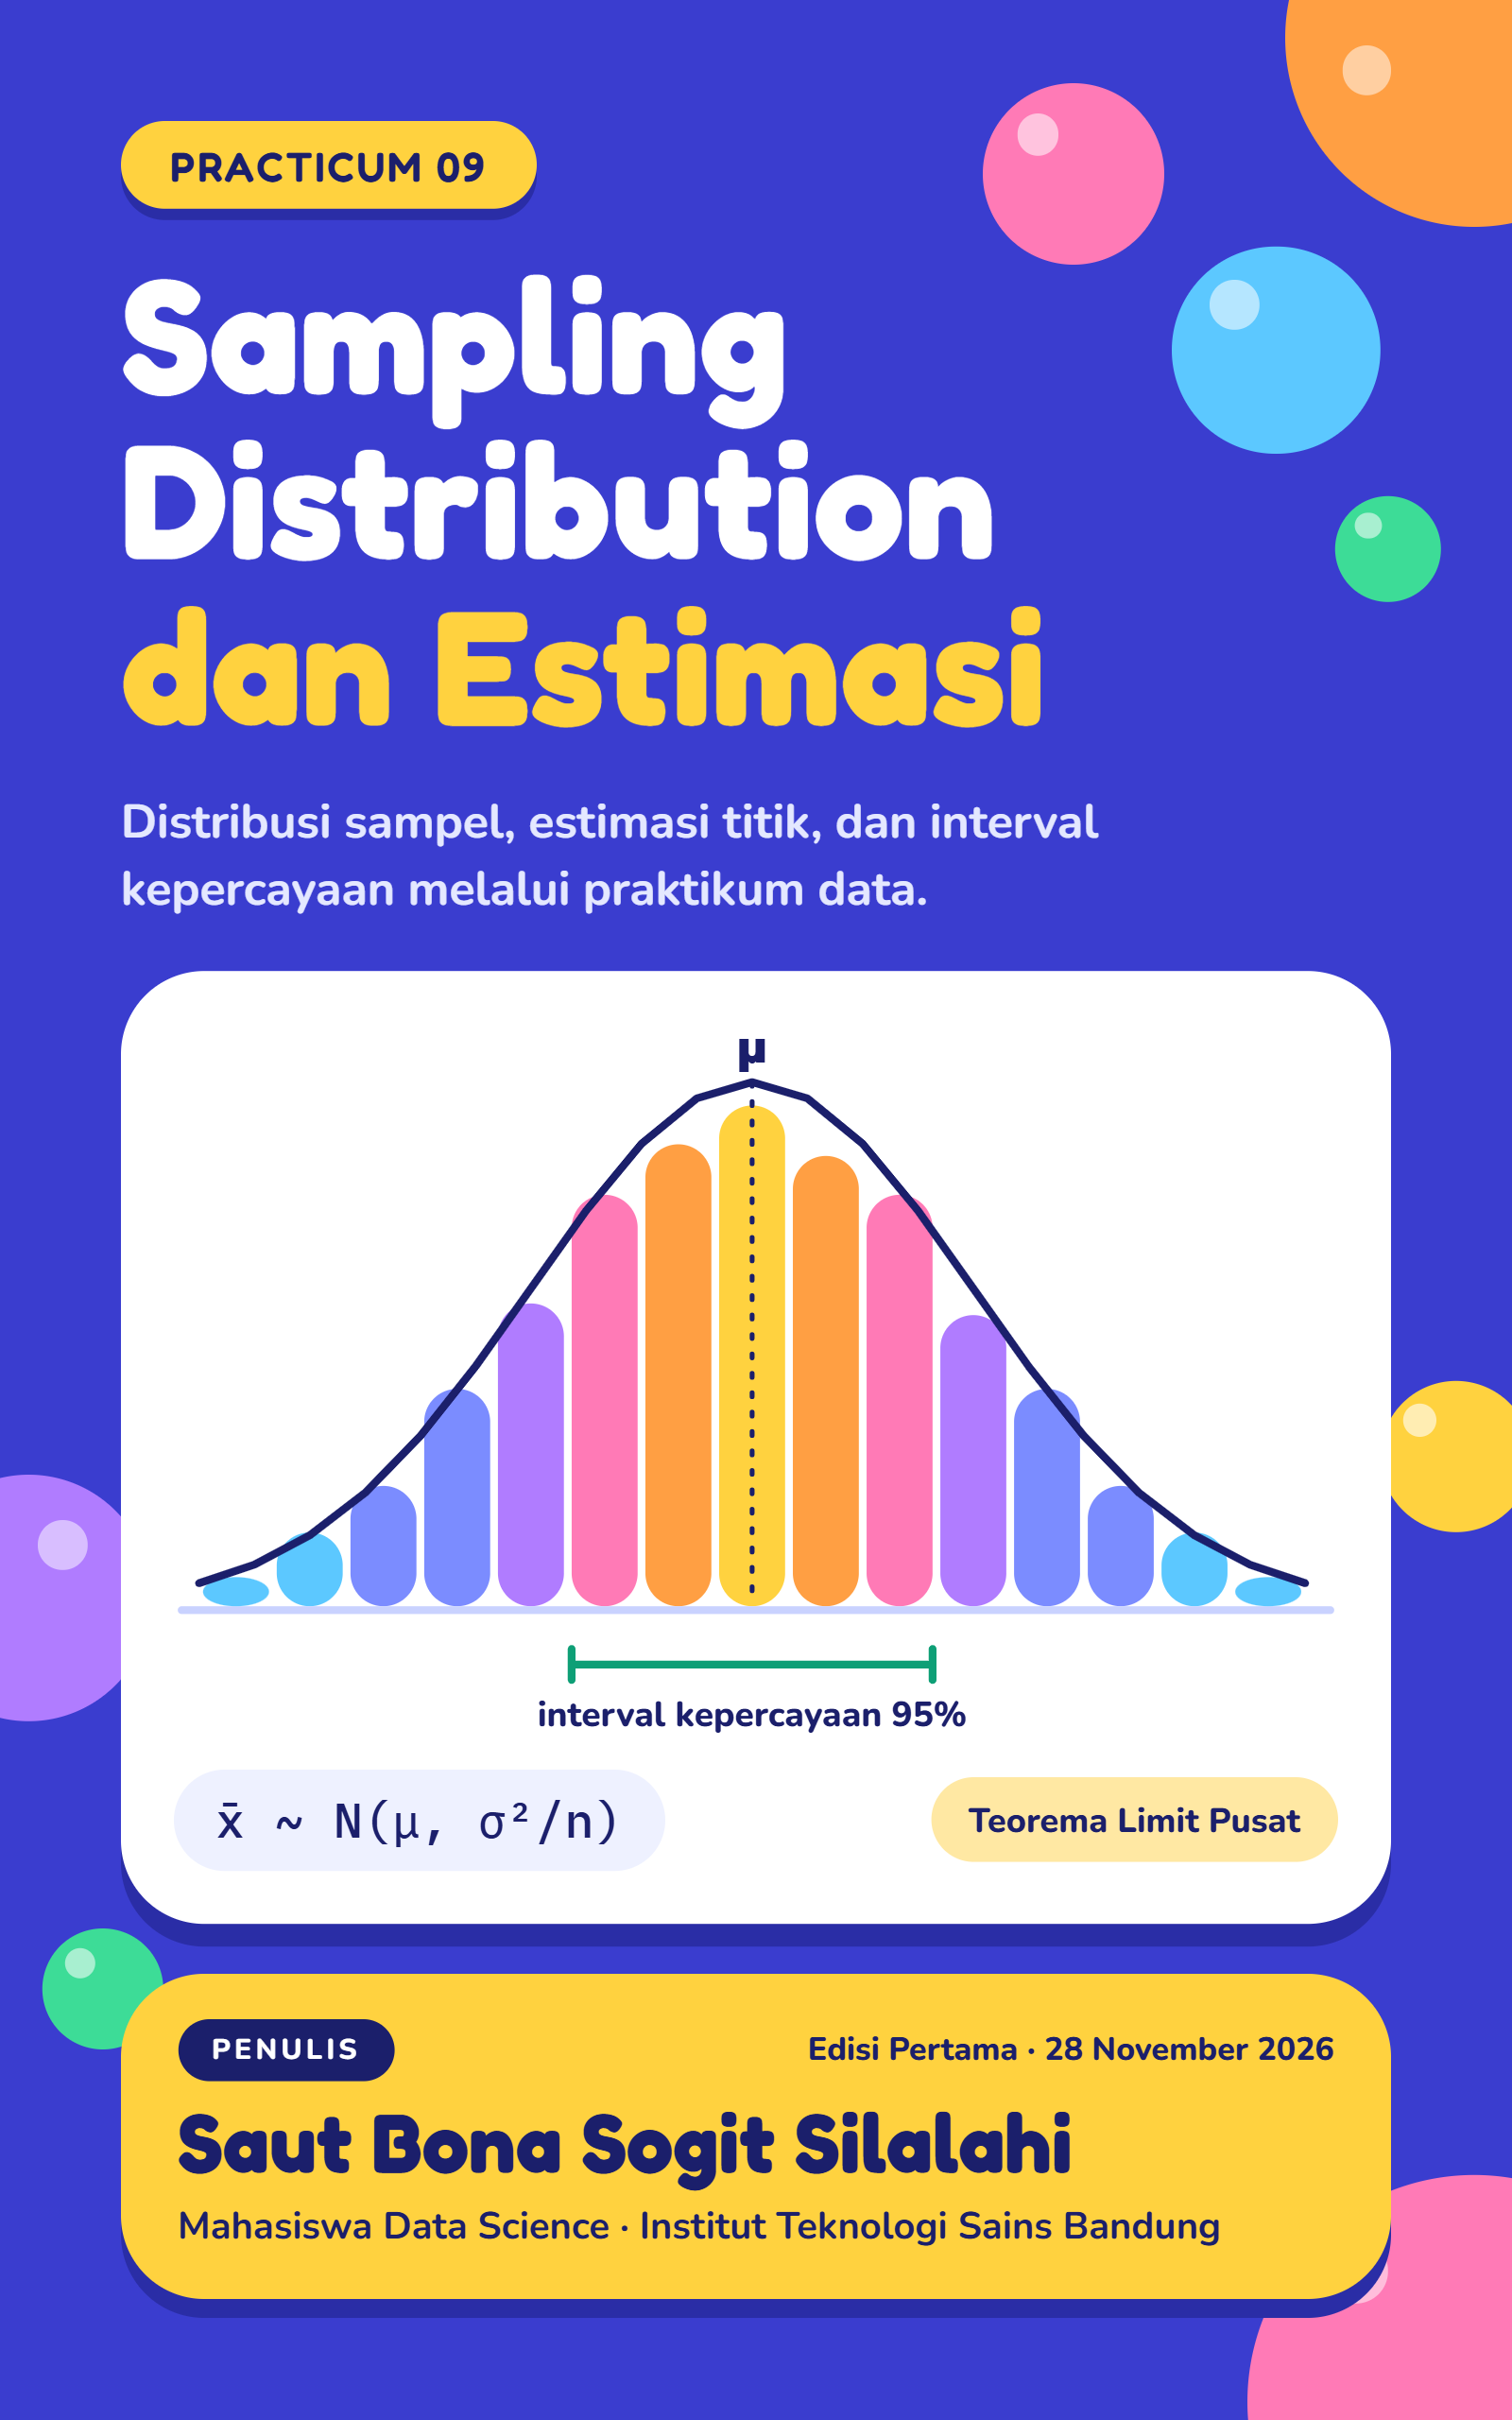
\includegraphics[height=\paperheight,keepaspectratio]{images/Cover.png}
  \end{titlepage}
  \restoregeometry
}

\usepackage{booktabs}
\usepackage{longtable}
\usepackage{array}
\usepackage{multirow}
\usepackage{wrapfig}
\usepackage{float}
\usepackage{colortbl}
\usepackage{pdflscape}
\usepackage{tabularx}
\usepackage{xltabular}
\usepackage{threeparttable}
\usepackage{threeparttablex}
\usepackage[normalem]{ulem}
\usepackage{makecell}
\usepackage{xcolor}
\makeatletter
\@ifpackageloaded{bookmark}{}{\usepackage{bookmark}}
\makeatother
\makeatletter
\@ifpackageloaded{caption}{}{\usepackage{caption}}
\AtBeginDocument{%
\ifdefined\contentsname
  \renewcommand*\contentsname{Daftar Isi}
\else
  \newcommand\contentsname{Daftar Isi}
\fi
\ifdefined\listfigurename
  \renewcommand*\listfigurename{Daftar Gambar}
\else
  \newcommand\listfigurename{Daftar Gambar}
\fi
\ifdefined\listtablename
  \renewcommand*\listtablename{Daftar Tabel}
\else
  \newcommand\listtablename{Daftar Tabel}
\fi
\ifdefined\figurename
  \renewcommand*\figurename{Gambar}
\else
  \newcommand\figurename{Gambar}
\fi
\ifdefined\tablename
  \renewcommand*\tablename{Tabel}
\else
  \newcommand\tablename{Tabel}
\fi
}
\@ifpackageloaded{float}{}{\usepackage{float}}
\floatstyle{ruled}
\@ifundefined{c@chapter}{\newfloat{codelisting}{h}{lop}}{\newfloat{codelisting}{h}{lop}[chapter]}
\floatname{codelisting}{Daftar}
\newcommand*\listoflistings{\listof{codelisting}{Daftar Daftar}}
\makeatother
\makeatletter
\makeatother
\makeatletter
\@ifpackageloaded{caption}{}{\usepackage{caption}}
\@ifpackageloaded{subcaption}{}{\usepackage{subcaption}}
\makeatother
\usepackage{bookmark}
\IfFileExists{xurl.sty}{\usepackage{xurl}}{} % add URL line breaks if available
\urlstyle{same}
% fallback for those not using the hyperref driver hyperxmp:
\makeatletter
\@ifundefined{xmpquote}{\newcommand{\xmpquote}[1]{#1}}{}
\makeatother
\hypersetup{
  pdftitle={Sains Data 2026},
  pdfauthor={Saut Bona Sogit Silalahi},
  pdflang={id},
  hidelinks,
  pdfcreator={LaTeX via pandoc}}


\title{Sains Data 2026}
\author{Saut Bona Sogit Silalahi}
\date{2026-11-28}
\begin{document}
\frontmatter
\maketitle

\renewcommand*\contentsname{Daftar Isi}
{
\setcounter{tocdepth}{2}
\tableofcontents
}

\mainmatter
\bookmarksetup{startatroot}

\chapter*{Kata Pengantar}\label{kata-pengantar}
\addcontentsline{toc}{chapter}{Kata Pengantar}

\markboth{Kata Pengantar}{Kata Pengantar}

Puji syukur kupanjatkan kepada Tuhan Yang Maha Esa, yang telah menuntun
jemari ini hingga sebuah buku kecil bernama \textbf{``Quarto Template''}
menemukan wujudnya. Kuserahkan ia kepada para pembaca dengan hati
lapang, bagi mahasiswa, dosen, peneliti, dan praktisi yang ingin menulis
dengan tertata, merawat naskahnya dengan sabar, lalu melepasnya ke dunia
dengan percaya diri.

Quarto adalah ruang menulis yang terbuka bagi siapa saja, sebuah
\emph{open-source scientific and technical publishing} tempat kata,
kode, angka, dan gambar duduk berdampingan dalam satu naskah. Layaknya
sungai yang berhulu satu namun bermuara ke banyak samudra, dari satu
tulisan ia mengalir menjadi HTML, PDF, Microsoft Word, dan berbagai
bentuk lainnya, tetap jernih dan dapat ditelusuri kembali ke asalnya.

Contoh sitasi: tuliskan \texttt{{[}@xie2015{]}} untuk merujuk entri
\texttt{xie2015} di \texttt{references/book.bib}. Pada hasil render,
sitasinya tampil seperti ini \citeproc{ref-xie2015}{{[}1{]}}.

Di halaman-halaman berikutnya, pembaca kuajak berjalan pelan menyusuri
jalan setapak: mengenal rumah bernama struktur proyek, menata pengaturan
di dalamnya, menuliskan kalimat dengan Markdown, menitipkan kode di
sela-sela cerita, merawat daftar pustaka, hingga \emph{merender}
semuanya menjadi karya yang siap dipersembahkan.

Setiap bagian kususun seperti jejak kaki di pasir basah, satu demi satu,
agar siapa pun yang baru pertama kali tiba di tepi Quarto tidak merasa
tersesat. Semoga contoh dan template di dalamnya menjadi lentera bagi
laporan penelitian, modul pembelajaran, buku elektronik, dan karya-karya
berbasis data yang kelak lahir dari tangan pembaca.

Harapku sederhana: semoga buku ini menjadi benih kecil yang tumbuh
menjadi kebiasaan menulis yang rapi, jujur, dan ilmiah, serta
menyuburkan literasi digital di sekitar kita. Lebih dari sekadar
petunjuk teknis, semoga ia membangkitkan rasa ingin tahu, dan mengantar
pembaca merancang template yang paling pas dengan langkahnya sendiri.

Kusadari tak ada karya yang tuntas tanpa celah. Karena itu pintu selalu
terbuka bagi kritik, saran, dan masukan, sebab dari situlah edisi-edisi
mendatang akan belajar tumbuh.

Akhir kata, semoga buku sederhana ini sampai ke tangan yang tepat,
menjadi teduh bagi yang mencari, dan menjadi setitik sumbangsih bagi
pendidikan, penelitian, dan ilmu pengetahuan.

\textbf{Saut Bona Sogit Silalahi}\\
Penulis

\section*{Penulis}\label{penulis}
\addcontentsline{toc}{section}{Penulis}

\markright{Penulis}

\begin{figure}[H]

{\centering 
\includegraphics[width=1.5in,height=\textheight,keepaspectratio]{images/author/Sogit.png}

}

\caption{Foto Saut Bona Sogit Silalahi}

\end{figure}%

\textbf{\href{https://www.linkedin.com/in/saut-bona-sogit-silalahi-7b0a45432/}{Saut
Bona Sogit Silalahi}} Mahasiswa Data Science di Institut Teknologi Sains
Bandung, dengan fokus pada pengolahan, eksplorasi, dan pemodelan data
untuk menghasilkan informasi yang bernilai.

\section*{Ucapan Terima Kasih}\label{ucapan-terima-kasih}
\addcontentsline{toc}{section}{Ucapan Terima Kasih}

\markright{Ucapan Terima Kasih}

Sebuah buku tak pernah tumbuh dari satu tangan saja. Ia berakar pada
banyak kebaikan yang diam-diam menopang, dan kepada merekalah
kusampaikan terima kasih yang paling tulus:

\begin{itemize}
\tightlist
\item
  \textbf{Keluarga}, rumah tempat aku selalu pulang, yang doa dan
  semangatnya menjadi penerang di sepanjang jalan, bahkan ketika langkah
  mulai lelah.
\item
  \textbf{Rekan-rekan dan para kolaborator}, yang dengan sabar
  menyumbangkan masukan, saran, dan kritik yang membangun, ibarat
  tangan-tangan yang membantu merapikan arah layar.
\item
  \textbf{\href{https://itsb.ac.id/}{ITSB}} dan segenap insan di
  dalamnya, yang membukakan ruang, sumber daya, dan fasilitas, sehingga
  benih gagasan ini punya tanah untuk tumbuh selama proses penelitian
  dan penulisan.
\end{itemize}

Kuharap Template eBook ini kelak menjadi teman yang berguna di meja baca
siapa pun yang membukanya, menghadirkan inspirasi dan secercah
pengetahuan baru. Semoga ia menjawab apa yang dicari para pembaca, dan
semoga setiap ilmu yang tersampaikan mengalir menjadi manfaat bagi
banyak orang.

\section*{Masukan \& Saran}\label{masukan-saran}
\addcontentsline{toc}{section}{Masukan \& Saran}

\markright{Masukan \& Saran}

Setiap masukan dan tanggapan darimu adalah cahaya kecil yang membantu
buku ini menemukan arah yang lebih baik. Bila ada yang ingin kamu
sampaikan, baik berupa saran, kritik, maupun sekadar sapaan, dengan
senang hati kunantikan lewat kontak di bawah ini.

\textbf{Email:} sogitsilalahi7@gmail.com

\bookmarksetup{startatroot}

\chapter{Sampling Distribution dan
Estimasi}\label{sampling-distribution-dan-estimasi}

Practicum 09: Sampling Distribution dan Estimasi

\hfill\break

Saut Bona Sogit Silalahi

LinkedIn {\textbar{}} GitHub {\textbar{}} Email

Mahasiswa Data Science di Institut Teknologi Sains Bandung, dengan fokus
pada pengolahan, eksplorasi, dan pemodelan data untuk menghasilkan
informasi yang bernilai.

\section{Tiga Distribusi yang Harus
Dibedakan}\label{tiga-distribusi-yang-harus-dibedakan}

{\def\LTcaptype{none} % do not increment counter
\begin{longtable}[]{@{}
  >{\raggedright\arraybackslash}p{(\linewidth - 6\tabcolsep) * \real{0.2500}}
  >{\raggedright\arraybackslash}p{(\linewidth - 6\tabcolsep) * \real{0.2500}}
  >{\raggedright\arraybackslash}p{(\linewidth - 6\tabcolsep) * \real{0.2500}}
  >{\raggedright\arraybackslash}p{(\linewidth - 6\tabcolsep) * \real{0.2500}}@{}}
\toprule\noalign{}
\begin{minipage}[b]{\linewidth}\raggedright
Distribusi
\end{minipage} & \begin{minipage}[b]{\linewidth}\raggedright
Isinya
\end{minipage} & \begin{minipage}[b]{\linewidth}\raggedright
Jumlah
\end{minipage} & \begin{minipage}[b]{\linewidth}\raggedright
nilai Contoh
\end{minipage} \\
\midrule\noalign{}
\endhead
\bottomrule\noalign{}
\endlastfoot
\textbf{Distribusi populasi} & Nilai \textbf{setiap unit} populasi &
\emph{N} & Pengeluaran 20.000 mahasiswa \\
\textbf{Distribusi sampel} & Nilai unit dalam \emph{satu sampel} &
\emph{n} & Pengeluaran 40 mahasiswa yang disurvei \\
\textbf{Distribusi sampling} & \textbf{Nilai statistik} (misalnya ) dari
̄𝑥\textbf{banyak sampel} & Sebanyak sampel yang (dibayangkan) diambil &
𝑥 dari 10.000 sampel berukuran 40 \\
\end{longtable}
}

Distribusi sampling adalah konsep \textbf{teoretis}: dalam praktik kita
hanya memiliki satu sampel. Namun dengan simulasi kita dapat
``melihatnya''.

\subsection{Populasi Simulasi}\label{populasi-simulasi}

Kita memakai populasi \textbf{20.000 mahasiswa} dengan variabel
\textbf{waktu layar harian} (jam) yang \textbf{menjulur kanan} - bentuk
yang sengaja dipilih jauh dari lonceng.

\begin{Shaded}
\begin{Highlighting}[]
\FunctionTok{set.seed}\NormalTok{(}\DecValTok{909}\NormalTok{)}
\NormalTok{N        }\OtherTok{\textless{}{-}} \DecValTok{20000}
\NormalTok{populasi }\OtherTok{\textless{}{-}} \FunctionTok{round}\NormalTok{(}\FunctionTok{rgamma}\NormalTok{(N, }\AttributeTok{shape =} \DecValTok{2}\NormalTok{, }\AttributeTok{rate =} \FloatTok{0.4}\NormalTok{), }\DecValTok{2}\NormalTok{) }\CommentTok{\# jam per hari}
\NormalTok{mu       }\OtherTok{\textless{}{-}} \FunctionTok{mean}\NormalTok{(populasi)}
\NormalTok{sigma    }\OtherTok{\textless{}{-}} \FunctionTok{sqrt}\NormalTok{(}\FunctionTok{mean}\NormalTok{((populasi }\SpecialCharTok{{-}}\NormalTok{ mu)}\SpecialCharTok{\^{}}\DecValTok{2}\NormalTok{))                 }\CommentTok{\# SD populasi (pembagi N)}
\FunctionTok{c}\NormalTok{(}\AttributeTok{N =}\NormalTok{ N, }\AttributeTok{mu =} \FunctionTok{round}\NormalTok{(mu, }\DecValTok{3}\NormalTok{), }\AttributeTok{sigma =} \FunctionTok{round}\NormalTok{(sigma, }\DecValTok{3}\NormalTok{))}
\end{Highlighting}
\end{Shaded}

\begin{verbatim}
        N        mu     sigma 
20000.000     5.010     3.551 
\end{verbatim}

\begin{quote}
\textbf{Interpretasi.} Populasi terdiri dari \emph{N} = 20.000 mahasiswa
dengan rata-rata waktu layar (𝜇) sekitar \textbf{5 jam per hari} dan
simpangan baku (𝜎) sekitar \textbf{3,5 jam}. Nilai ini sesuai dengan
sifat distribusi gamma yang dibangkitkan (mean = shape/rate = 2/0,4 = 5;
SD = √2/0,4 ≈ 3,54). 𝜎 yang hampir sebesar 𝜇 menandakan data sangat
beragam dan menjulur kanan. Kedua angka ini adalah \textbf{parameter}
populasi, yaitu nilai ``kebenaran'' yang nanti akan ditaksir dari
sampel.
\end{quote}

\begin{Shaded}
\begin{Highlighting}[]
\FunctionTok{set.seed}\NormalTok{(}\DecValTok{1}\NormalTok{)}
\NormalTok{satu\_sampel }\OtherTok{\textless{}{-}} \FunctionTok{sample}\NormalTok{(populasi, }\DecValTok{40}\NormalTok{)}
\NormalTok{banyak\_rata }\OtherTok{\textless{}{-}} \FunctionTok{replicate}\NormalTok{(}\DecValTok{10000}\NormalTok{, }\FunctionTok{mean}\NormalTok{(}\FunctionTok{sample}\NormalTok{(populasi, }\DecValTok{40}\NormalTok{)))}
\FunctionTok{par}\NormalTok{(}\AttributeTok{mfrow =} \FunctionTok{c}\NormalTok{(}\DecValTok{1}\NormalTok{, }\DecValTok{3}\NormalTok{))}
\FunctionTok{hist}\NormalTok{(populasi, }\AttributeTok{breaks    =} \DecValTok{40}\NormalTok{, }\AttributeTok{col =} \StringTok{"\#9ecae1"}\NormalTok{, }\AttributeTok{border =} \StringTok{"white"}\NormalTok{, }\AttributeTok{main =} \StringTok{"Populasi (N= 20.000)"}\NormalTok{,}
\AttributeTok{xlab =} \StringTok{"Jam per hari"}\NormalTok{, }\AttributeTok{xlim =} \FunctionTok{c}\NormalTok{(}\DecValTok{0}\NormalTok{, }\DecValTok{20}\NormalTok{))}
\FunctionTok{hist}\NormalTok{(satu\_sampel, }\AttributeTok{breaks =} \DecValTok{12}\NormalTok{, }\AttributeTok{col =} \StringTok{"\#fdae6b"}\NormalTok{, }\AttributeTok{border =} \StringTok{"white"}\NormalTok{, }\AttributeTok{main =} \StringTok{"Satu sampel (n = 40)"}\NormalTok{,}
\AttributeTok{xlab =} \StringTok{"Jam per hari"}\NormalTok{, }\AttributeTok{xlim =} \FunctionTok{c}\NormalTok{(}\DecValTok{0}\NormalTok{, }\DecValTok{20}\NormalTok{))}
\FunctionTok{hist}\NormalTok{(banyak\_rata, }\AttributeTok{breaks =} \DecValTok{40}\NormalTok{, }\AttributeTok{col =} \StringTok{"\#a1d99b"}\NormalTok{, }\AttributeTok{border =} \StringTok{"white"}\NormalTok{,}
\AttributeTok{main =} \StringTok{"Sampling distribution x{-}bar"}\NormalTok{, }\AttributeTok{xlab =} \StringTok{"Rata{-}rata sampel (n = 40)"}\NormalTok{)}
\end{Highlighting}
\end{Shaded}

\pandocbounded{\includegraphics[keepaspectratio]{chapters/bab-1_files/figure-pdf/unnamed-chunk-2-1.pdf}}

\begin{Shaded}
\begin{Highlighting}[]
\FunctionTok{par}\NormalTok{(}\AttributeTok{mfrow =} \FunctionTok{c}\NormalTok{(}\DecValTok{1}\NormalTok{, }\DecValTok{1}\NormalTok{))}
\end{Highlighting}
\end{Shaded}

Populasi dan satu sampel sama-sama menjulur kanan, tetapi distribusi
rata-rata sampel jauh lebih sempit dan hampir berbentuk lonceng. Inilah
inti pertemuan ini.

\begin{quote}
\textbf{Interpretasi.} Histogram biru (populasi) dan oranye (satu
sampel, \emph{n} = 40) sama-sama berbentuk miring ke kanan: sebagian
besar mahasiswa memiliki waktu layar rendah sampai sedang, dan sedikit
orang memiliki waktu layar yang sangat panjang. Histogram oranye lebih
``kasar'' karena hanya berisi 40 data, tetapi masih meniru bentuk
populasi. Histogram hijau (distribusi sampling 𝑥̄) berbeda: bentuknya
simetris menyerupai lonceng, terpusat di sekitar 𝜇 ≈ 5 jam, dan
sebarannya jauh lebih sempit (sekitar 4 sampai 6 jam, sedangkan data
individu berkisar 0 sampai lebih dari 15 jam). Artinya rata-rata sampel
jauh lebih stabil daripada nilai individu, dan bentuknya normal walaupun
populasinya tidak.
\end{quote}

\section{Distribusi Sampling Rata-rata
Sampel}\label{distribusi-sampling-rata-rata-sampel}

Untuk sampel acak berukuran 𝑛 dari populasi dengan mean 𝜇 dan simpangan
baku 𝜎:

{\def\LTcaptype{none} % do not increment counter
\begin{longtable}[]{@{}
  >{\raggedright\arraybackslash}p{(\linewidth - 4\tabcolsep) * \real{0.3333}}
  >{\raggedright\arraybackslash}p{(\linewidth - 4\tabcolsep) * \real{0.3333}}
  >{\raggedright\arraybackslash}p{(\linewidth - 4\tabcolsep) * \real{0.3333}}@{}}
\toprule\noalign{}
\begin{minipage}[b]{\linewidth}\raggedright
Sifat
\end{minipage} & \begin{minipage}[b]{\linewidth}\raggedright
Rumus
\end{minipage} & \begin{minipage}[b]{\linewidth}\raggedright
Arti
\end{minipage} \\
\midrule\noalign{}
\endhead
\bottomrule\noalign{}
\endlastfoot
\textbf{Mean} & 𝜇 ̄𝑥 = � & 𝑥 adalah penaksir tak \textbf{bias}:
rata-ratanya tepat di parameter \\
\textbf{Standard error} & 𝜎 ̄𝑥 =𝜎√� & Sebaran ̄𝑥 mengecil seiring
bertambahnya \emph{n} \\
\textbf{Bentuk } & Normal jika populasi normal;mendekati normal untuk 𝑛
cukup besar (CLT) & Memungkinkan perhitungan peluang \\
\end{longtable}
}

\begin{Shaded}
\begin{Highlighting}[]
\NormalTok{knitr}\SpecialCharTok{::}\FunctionTok{kable}\NormalTok{(}\FunctionTok{data.frame}\NormalTok{(}
\AttributeTok{Besaran =} \FunctionTok{c}\NormalTok{(}\StringTok{"Mean distribusi sampling"}\NormalTok{, }\StringTok{"SD distribusi sampling (SE)"}\NormalTok{),}
\AttributeTok{Teori =} \FunctionTok{round}\NormalTok{(}\FunctionTok{c}\NormalTok{(mu, sigma }\SpecialCharTok{/} \FunctionTok{sqrt}\NormalTok{(}\DecValTok{40}\NormalTok{)), }\DecValTok{4}\NormalTok{),}
\AttributeTok{Simulasi\_10000\_sampel =} \FunctionTok{round}\NormalTok{(}\FunctionTok{c}\NormalTok{(}\FunctionTok{mean}\NormalTok{(banyak\_rata), }\FunctionTok{sd}\NormalTok{(banyak\_rata)), }\DecValTok{4}\NormalTok{)}
\NormalTok{), }\AttributeTok{caption =} \StringTok{"Teori vs simulasi untuk n = 40"}\NormalTok{)}
\end{Highlighting}
\end{Shaded}

\begin{longtable}[]{@{}lrr@{}}
\caption{Teori vs simulasi untuk n = 40}\tabularnewline
\toprule\noalign{}
Besaran & Teori & Simulasi\_10000\_sampel \\
\midrule\noalign{}
\endfirsthead
\toprule\noalign{}
Besaran & Teori & Simulasi\_10000\_sampel \\
\midrule\noalign{}
\endhead
\bottomrule\noalign{}
\endlastfoot
Mean distribusi sampling & 5.0097 & 5.0024 \\
SD distribusi sampling (SE) & 0.5615 & 0.5556 \\
\end{longtable}

Hasil simulasi hampir persis sama dengan teori.

\begin{quote}
\textbf{Interpretasi.} Mean distribusi sampling dari 10.000 sampel
(kolom simulasi) hampir sama dengan 𝜇 (kolom teori, sekitar 5), yang
membuktikan bahwa 𝑥̄ adalah penaksir \textbf{tak bias}: rata-ratanya
tepat sasaran. Simpangan baku distribusi sampling (standard error)
secara teori 𝜎/√40 ≈ 3,54/6,32 ≈ \textbf{0,56 jam}, dan hasil simulasi
nyaris identik. Jadi rumus SE = 𝜎/√𝑛 benar, dan satu rata-rata sampel
berukuran 40 biasanya meleset sekitar 0,56 jam dari 𝜇.
\end{quote}

Koreksi populasi terhingga. Rumus 𝜎/√𝑛 mengasumsikan populasi sangat
besar dibanding sampel. Jika sampel mencapai lebih dari sekitar 5\%
populasi (tanpa pengembalian), SE dikalikan faktor √𝑁−𝑛𝑁−1 . Pada contoh
ini 𝑛/𝑁 = 0,2\%, sehingga koreksi dapat diabaikan.

\subsection{Pengaruh Ukuran Sampel}\label{pengaruh-ukuran-sampel}

\begin{Shaded}
\begin{Highlighting}[]
\FunctionTok{set.seed}\NormalTok{(}\DecValTok{2}\NormalTok{)}
\NormalTok{n\_list }\OtherTok{\textless{}{-}} \FunctionTok{c}\NormalTok{(}\DecValTok{5}\NormalTok{, }\DecValTok{20}\NormalTok{, }\DecValTok{80}\NormalTok{)}
\FunctionTok{par}\NormalTok{(}\AttributeTok{mfrow =} \FunctionTok{c}\NormalTok{(}\DecValTok{1}\NormalTok{, }\DecValTok{3}\NormalTok{))}
\ControlFlowTok{for}\NormalTok{ (nn }\ControlFlowTok{in}\NormalTok{ n\_list) \{}
\NormalTok{rata }\OtherTok{\textless{}{-}} \FunctionTok{replicate}\NormalTok{(}\DecValTok{5000}\NormalTok{, }\FunctionTok{mean}\NormalTok{(}\FunctionTok{sample}\NormalTok{(populasi, nn)))}
\FunctionTok{hist}\NormalTok{(rata, }\AttributeTok{breaks =} \DecValTok{40}\NormalTok{, }\AttributeTok{col =} \StringTok{"\#a1d99b"}\NormalTok{, }\AttributeTok{border =} \StringTok{"white"}\NormalTok{, }\AttributeTok{xlim =} \FunctionTok{c}\NormalTok{(}\DecValTok{1}\NormalTok{, }\DecValTok{10}\NormalTok{), }\AttributeTok{freq=} \ConstantTok{FALSE}\NormalTok{,}
\AttributeTok{main =} \FunctionTok{paste0}\NormalTok{(}\StringTok{"n = "}\NormalTok{, nn, }\StringTok{" (SE = "}\NormalTok{, }\FunctionTok{round}\NormalTok{(sigma }\SpecialCharTok{/} \FunctionTok{sqrt}\NormalTok{(nn), }\DecValTok{2}\NormalTok{), }\StringTok{")"}\NormalTok{),}
\AttributeTok{xlab =} \StringTok{"Rata{-}rata sampel"}\NormalTok{)}
\FunctionTok{curve}\NormalTok{(}\FunctionTok{dnorm}\NormalTok{(x, mu, sigma }\SpecialCharTok{/} \FunctionTok{sqrt}\NormalTok{(nn)), }\AttributeTok{add =} \ConstantTok{TRUE}\NormalTok{, }\AttributeTok{col =} \StringTok{"firebrick"}\NormalTok{, }\AttributeTok{lwd =} \DecValTok{2}\NormalTok{)}
\FunctionTok{abline}\NormalTok{(}\AttributeTok{v =}\NormalTok{ mu, }\AttributeTok{lty =} \DecValTok{2}\NormalTok{)}
\NormalTok{\}}
\end{Highlighting}
\end{Shaded}

\pandocbounded{\includegraphics[keepaspectratio]{chapters/bab-1_files/figure-pdf/unnamed-chunk-5-1.pdf}}

\begin{Shaded}
\begin{Highlighting}[]
\FunctionTok{par}\NormalTok{(}\AttributeTok{mfrow =} \FunctionTok{c}\NormalTok{(}\DecValTok{1}\NormalTok{, }\DecValTok{1}\NormalTok{))}
\end{Highlighting}
\end{Shaded}

Kurva merah adalah distribusi normal dengan mean 𝜇 dan SD 𝜎/√𝑛. Semakin
besar 𝑛: (1) distribusi semakin \textbf{sempit}, dan (2) bentuknya
semakin \textbf{mendekati normal} meskipun populasinya menjulur kanan.

\begin{quote}
\textbf{Interpretasi.} Pada \emph{n} = 5 (SE ≈ 1,58) histogram masih
sedikit miring ke kanan dan kurva normal belum pas sempurna. Pada
\emph{n} = 20 (SE ≈ 0,79) bentuknya sudah jauh lebih simetris, dan pada
\emph{n} = 80 (SE ≈ 0,40) histogram hampir berimpit dengan kurva merah.
Garis putus-putus (𝜇) selalu berada di pusat, sehingga ukuran sampel
tidak mengubah \textbf{pusat} distribusi (tetap tak bias), tetapi
mengecilkan \textbf{sebaran} dan memperbaiki \textbf{kenormalan}. Ketika
\emph{n} naik 4 kali lipat dari 5 ke 20 dan dari 20 ke 80, SE turun
kira-kira separuhnya (1,58 → 0,79 → 0,40), sesuai hukum akar kuadrat.
\end{quote}

\section{Central Limit Theorem (CLT)}\label{central-limit-theorem-clt}

\textbf{Central Limit Theorem}. Jika sampel acak berukuran 𝑛 diambil
dari populasi \textbf{sembarang bentuk} dengan mean 𝜇 dan simpangan baku
𝜎 (terhingga), maka untuk 𝑛 yang cukup besar, distribusi sampling ̄𝑥
\textbf{mendekati normal}

\[\bar{x} \approx N\left(\mu, \frac{\sigma}{\sqrt{n}}\right)\]

CLT adalah alasan mengapa distribusi normal muncul di mana-mana dalam
statistika inferensial--bukan karena data selalu normal, tetapi karena
\textbf{rata-rata} dari data cenderung normal.

\subsection{Demonstrasi pada Tiga Bentuk
Populasi}\label{demonstrasi-pada-tiga-bentuk-populasi}

\begin{Shaded}
\begin{Highlighting}[]
\FunctionTok{set.seed}\NormalTok{(}\DecValTok{3}\NormalTok{)}
\NormalTok{pop\_bentuk }\OtherTok{\textless{}{-}} \FunctionTok{list}\NormalTok{(}
\StringTok{"Seragam"} \OtherTok{=} \FunctionTok{runif}\NormalTok{(}\DecValTok{20000}\NormalTok{, }\DecValTok{0}\NormalTok{, }\DecValTok{10}\NormalTok{),}
\StringTok{"Menjulur kanan"} \OtherTok{=} \FunctionTok{rexp}\NormalTok{(}\DecValTok{20000}\NormalTok{, }\AttributeTok{rate =} \FloatTok{0.5}\NormalTok{),}
\StringTok{"Bimodal"} \OtherTok{=} \FunctionTok{c}\NormalTok{(}\FunctionTok{rnorm}\NormalTok{(}\DecValTok{10000}\NormalTok{, }\DecValTok{2}\NormalTok{, }\FloatTok{0.8}\NormalTok{), }\FunctionTok{rnorm}\NormalTok{(}\DecValTok{10000}\NormalTok{, }\DecValTok{8}\NormalTok{, }\FloatTok{0.8}\NormalTok{))}
\NormalTok{)}
\NormalTok{ukuran }\OtherTok{\textless{}{-}} \FunctionTok{c}\NormalTok{(}\DecValTok{2}\NormalTok{, }\DecValTok{5}\NormalTok{, }\DecValTok{30}\NormalTok{)}
\FunctionTok{par}\NormalTok{(}\AttributeTok{mfrow =} \FunctionTok{c}\NormalTok{(}\DecValTok{4}\NormalTok{, }\DecValTok{3}\NormalTok{), }\AttributeTok{mar =} \FunctionTok{c}\NormalTok{(}\DecValTok{3}\NormalTok{, }\DecValTok{3}\NormalTok{, }\FloatTok{2.5}\NormalTok{, }\DecValTok{1}\NormalTok{))}
\ControlFlowTok{for}\NormalTok{ (nama }\ControlFlowTok{in} \FunctionTok{names}\NormalTok{(pop\_bentuk)) \{}
\FunctionTok{hist}\NormalTok{(pop\_bentuk[[nama]], }\AttributeTok{breaks =} \DecValTok{40}\NormalTok{, }\AttributeTok{col =} \StringTok{"\#9ecae1"}\NormalTok{, }\AttributeTok{border =} \StringTok{"white"}\NormalTok{,}
\AttributeTok{main =} \FunctionTok{paste}\NormalTok{(}\StringTok{"Populasi:"}\NormalTok{, nama), }\AttributeTok{xlab =} \StringTok{""}\NormalTok{, }\AttributeTok{ylab =} \StringTok{""}\NormalTok{)}
\NormalTok{\}}
\ControlFlowTok{for}\NormalTok{ (nn }\ControlFlowTok{in}\NormalTok{ ukuran) \{}
\ControlFlowTok{for}\NormalTok{ (nama }\ControlFlowTok{in} \FunctionTok{names}\NormalTok{(pop\_bentuk)) \{}
\NormalTok{rata }\OtherTok{\textless{}{-}} \FunctionTok{replicate}\NormalTok{(}\DecValTok{3000}\NormalTok{, }\FunctionTok{mean}\NormalTok{(}\FunctionTok{sample}\NormalTok{(pop\_bentuk[[nama]], nn)))}
\FunctionTok{hist}\NormalTok{(rata, }\AttributeTok{breaks =} \DecValTok{35}\NormalTok{, }\AttributeTok{col =} \StringTok{"\#a1d99b"}\NormalTok{, }\AttributeTok{border =} \StringTok{"white"}\NormalTok{,}
\AttributeTok{main =} \FunctionTok{paste0}\NormalTok{(nama, }\StringTok{", n = "}\NormalTok{, nn), }\AttributeTok{xlab =} \StringTok{""}\NormalTok{, }\AttributeTok{ylab =} \StringTok{""}\NormalTok{)}
\NormalTok{\}}
\NormalTok{\}}
\end{Highlighting}
\end{Shaded}

\pandocbounded{\includegraphics[keepaspectratio]{chapters/bab-1_files/figure-pdf/unnamed-chunk-7-1.pdf}}

\begin{Shaded}
\begin{Highlighting}[]
\FunctionTok{par}\NormalTok{(}\AttributeTok{mfrow =} \FunctionTok{c}\NormalTok{(}\DecValTok{1}\NormalTok{, }\DecValTok{1}\NormalTok{), }\AttributeTok{mar =} \FunctionTok{c}\NormalTok{(}\DecValTok{5}\NormalTok{, }\DecValTok{4}\NormalTok{, }\DecValTok{4}\NormalTok{, }\DecValTok{2}\NormalTok{) }\SpecialCharTok{+} \FloatTok{0.1}\NormalTok{)}
\end{Highlighting}
\end{Shaded}

Baris pertama adalah populasi; baris berikutnya adalah distribusi
sampling ̄𝑥 untuk 𝑛 = 2, 5, dan 30. Populasi seragam sudah tampak
lonceng pada 𝑛 = 5; populasi bimodal masih bergelombang pada 𝑛 = 2
tetapi lonceng pada 𝑛 = 30; populasi menjulur kanan membutuhkan 𝑛
terbesar untuk menghilangkan kemencengannya.

\begin{quote}
\textbf{Interpretasi.} Tiga populasi di baris pertama sangat berbeda:
datar (seragam), miring tajam (eksponensial), dan berpuncak dua
(bimodal). Namun pada \emph{n} = 30 ketiga distribusi rata-rata sampel
tampak simetris berbentuk lonceng. Ini adalah inti CLT: bentuk populasi
``dilupakan'' ketika kita beralih ke distribusi rata-rata. Bedanya hanya
pada \textbf{kecepatan} konvergensi: populasi seragam (simetris) cepat
normal, bimodal baru menyatu setelah \emph{n} cukup besar karena dua
puncaknya harus ``terhapus'', dan eksponensial paling lambat karena
kemencengannya paling kuat. Kesimpulannya, CLT berlaku untuk populasi
apa pun, tetapi kata ``cukup besar'' bergantung pada bentuk populasi.
\end{quote}

\subsection{Seberapa Besar ``Cukup
Besar''?}\label{seberapa-besar-cukup-besar}

{\def\LTcaptype{none} % do not increment counter
\begin{longtable}[]{@{}ll@{}}
\toprule\noalign{}
Bentuk populasi & Ukuran sampel yang biasanya cukup \\
\midrule\noalign{}
\endhead
\bottomrule\noalign{}
\endlastfoot
Normal & Berapa pun (distribusi ̄𝑥 tepat normal \\
Simetris, tidak normal & Sekitar 10--15 \\
Menceng sedang & Sekitar 30 (aturan praktis yang populer) \\
Sangat menceng atau banyak outlier & Bisa jauh lebih dari 30 \\
\end{longtable}
}

\begin{Shaded}
\begin{Highlighting}[]
\NormalTok{skew }\OtherTok{\textless{}{-}} \ControlFlowTok{function}\NormalTok{(x) \{ d }\OtherTok{\textless{}{-}}\NormalTok{ x }\SpecialCharTok{{-}} \FunctionTok{mean}\NormalTok{(x); }\FunctionTok{mean}\NormalTok{(d}\SpecialCharTok{\^{}}\DecValTok{3}\NormalTok{) }\SpecialCharTok{/} \FunctionTok{mean}\NormalTok{(d}\SpecialCharTok{\^{}}\DecValTok{2}\NormalTok{)}\SpecialCharTok{\^{}}\FloatTok{1.5}\NormalTok{ \}}
\FunctionTok{set.seed}\NormalTok{(}\DecValTok{4}\NormalTok{)}
\FunctionTok{data.frame}\NormalTok{(}\AttributeTok{n =} \FunctionTok{c}\NormalTok{(}\DecValTok{2}\NormalTok{, }\DecValTok{5}\NormalTok{, }\DecValTok{10}\NormalTok{, }\DecValTok{30}\NormalTok{, }\DecValTok{100}\NormalTok{),}
\AttributeTok{Kemencengan\_xbar =} \FunctionTok{sapply}\NormalTok{(}\FunctionTok{c}\NormalTok{(}\DecValTok{2}\NormalTok{, }\DecValTok{5}\NormalTok{, }\DecValTok{10}\NormalTok{, }\DecValTok{30}\NormalTok{, }\DecValTok{100}\NormalTok{), }\ControlFlowTok{function}\NormalTok{(nn)}
\FunctionTok{round}\NormalTok{(}\FunctionTok{skew}\NormalTok{(}\FunctionTok{replicate}\NormalTok{(}\DecValTok{5000}\NormalTok{, }\FunctionTok{mean}\NormalTok{(}\FunctionTok{sample}\NormalTok{(populasi, nn)))), }\DecValTok{3}\NormalTok{)))}
\end{Highlighting}
\end{Shaded}

\begin{verbatim}
    n Kemencengan_xbar
1   2            1.007
2   5            0.581
3  10            0.470
4  30            0.220
5 100            0.170
\end{verbatim}

Kemencengan distribusi ̄𝑥 menyusut kira-kira sebanding dengan 1/√𝑛.

\begin{quote}
\textbf{Interpretasi.} Kemencengan (\emph{skewness}) populasi gamma ini
sekitar 1,41, yaitu menceng kuat ke kanan. Kemencengan distribusi 𝑥̄
turun terus seiring bertambahnya \emph{n}: kira-kira 1,0 pada \emph{n} =
2, 0,6 pada \emph{n} = 5, 0,45 pada \emph{n} = 10, 0,26 pada \emph{n} =
30, dan 0,14 pada \emph{n} = 100 (nilai simulasi akan sedikit berbeda
karena acak). Nilai di sekitar 0 berarti simetris. Pada \emph{n} = 30
kemencengan masih sekitar 0,26, jadi aturan ``30 sudah cukup'' bekerja
untuk menceng sedang, tetapi untuk data sangat menceng seperti ini baru
benar-benar mendekati simetris pada \emph{n} yang lebih besar (sekitar
100).
\end{quote}

\subsection{Menghitung Peluang dengan
CLT}\label{menghitung-peluang-dengan-clt}

\textbf{Contoh}: Jika diambil sampel acak 40 mahasiswa, berapa peluang
rata-rata waktu layarnya melebihi 5,5 jam?

\[z = \frac{\bar{x} - \mu}{\sigma / \sqrt{n}} \qquad P(\bar{x} > 5,5) = P(Z > z)\]

\begin{Shaded}
\begin{Highlighting}[]
\NormalTok{se40 }\OtherTok{\textless{}{-}}\NormalTok{ sigma }\SpecialCharTok{/} \FunctionTok{sqrt}\NormalTok{(}\DecValTok{40}\NormalTok{)}
\NormalTok{z\_55 }\OtherTok{\textless{}{-}}\NormalTok{ (}\FloatTok{5.5} \SpecialCharTok{{-}}\NormalTok{ mu) }\SpecialCharTok{/}\NormalTok{ se40}
\FunctionTok{c}\NormalTok{(}\AttributeTok{SE =} \FunctionTok{round}\NormalTok{(se40, }\DecValTok{4}\NormalTok{), }\AttributeTok{z =} \FunctionTok{round}\NormalTok{(z\_55, }\DecValTok{3}\NormalTok{),}
\AttributeTok{Peluang\_CLT =} \FunctionTok{round}\NormalTok{(}\DecValTok{1} \SpecialCharTok{{-}} \FunctionTok{pnorm}\NormalTok{(z\_55), }\DecValTok{4}\NormalTok{),}
\AttributeTok{Peluang\_simulasi =} \FunctionTok{round}\NormalTok{(}\FunctionTok{mean}\NormalTok{(banyak\_rata }\SpecialCharTok{\textgreater{}} \FloatTok{5.5}\NormalTok{), }\DecValTok{4}\NormalTok{))}
\end{Highlighting}
\end{Shaded}

\begin{verbatim}
              SE                z      Peluang_CLT Peluang_simulasi 
          0.5615           0.8730           0.1913           0.1803 
\end{verbatim}

\begin{quote}
\textbf{Interpretasi.} Dengan SE ≈ 0,56, nilai 5,5 jam berada sekitar
\textbf{z ≈ 0,89} simpangan baku di atas 𝜇. Peluang CLT bahwa rata-rata
40 mahasiswa melebihi 5,5 jam adalah sekitar \textbf{0,19 (±19\%)}.
Peluang hasil simulasi 10.000 sampel hampir sama dengan angka CLT,
sehingga pendekatan normal dapat dipercaya pada \emph{n} = 40 walaupun
populasinya menceng. Selisih kecil antara keduanya wajar karena simulasi
mengandung kesalahan acak dan sedikit sisa kemencengan.
\end{quote}

Perbandingan: peluang seorang mahasiswa (bukan rata-rata 40 orang)
memiliki waktu layar di atas 5,5 jam jauh lebih besar:

\begin{Shaded}
\begin{Highlighting}[]
\FunctionTok{mean}\NormalTok{(populasi }\SpecialCharTok{\textgreater{}} \FloatTok{5.5}\NormalTok{)}
\end{Highlighting}
\end{Shaded}

\begin{verbatim}
[1] 0.35175
\end{verbatim}

\begin{quote}
\textbf{Interpretasi.} Sekitar \textbf{35\%} mahasiswa secara individu
memiliki waktu layar di atas 5,5 jam, hampir dua kali lipat dari peluang
untuk \textbf{rata-rata} 40 mahasiswa (sekitar 19\%). Alasannya, nilai
individu sangat bervariasi (SD ≈ 3,5), sedangkan rata-rata kelompok
``menyaring'' nilai ekstrem sehingga jauh lebih terkonsentrasi di
sekitar 5. Jadi peluang untuk individu dan peluang untuk rata-rata tidak
boleh dicampur.
\end{quote}

Individu sangat bervariasi, tetapi \textbf{rata-rata} dari banyak
individu jauh lebih stabil.

\section{Distribusi Sampling Proporsi
Sampel}\label{distribusi-sampling-proporsi-sampel}

Untuk variabel kategorik biner (Ya/Tidak), statistik yang dipakai adalah
proporsi sampel ̂𝑝 = 𝑥/𝑛.

\begin{Shaded}
\begin{Highlighting}[]
\FunctionTok{library}\NormalTok{(knitr)}
\FunctionTok{library}\NormalTok{(kableExtra)}

\NormalTok{tabel\_proporsi }\OtherTok{\textless{}{-}} \FunctionTok{data.frame}\NormalTok{(}
  \AttributeTok{Sifat =} \FunctionTok{c}\NormalTok{(}\StringTok{"Mean"}\NormalTok{, }\StringTok{"Standard error"}\NormalTok{, }\StringTok{"Bentuk"}\NormalTok{),}
  \AttributeTok{Rumus =} \FunctionTok{c}\NormalTok{(}
    \StringTok{"$}\SpecialCharTok{\textbackslash{}\textbackslash{}}\StringTok{mu\_\{}\SpecialCharTok{\textbackslash{}\textbackslash{}}\StringTok{hat\{p\}\} = p$"}\NormalTok{,}
    \StringTok{"$}\SpecialCharTok{\textbackslash{}\textbackslash{}}\StringTok{sigma\_\{}\SpecialCharTok{\textbackslash{}\textbackslash{}}\StringTok{hat\{p\}\} = }\SpecialCharTok{\textbackslash{}\textbackslash{}}\StringTok{sqrt\{}\SpecialCharTok{\textbackslash{}\textbackslash{}}\StringTok{dfrac\{p(1{-}p)\}\{n\}\}$"}\NormalTok{,}
    \StringTok{"Mendekati normal jika $np }\SpecialCharTok{\textbackslash{}\textbackslash{}}\StringTok{ge 10$ **dan** $n(1{-}p) }\SpecialCharTok{\textbackslash{}\textbackslash{}}\StringTok{ge 10$"}
\NormalTok{  )}
\NormalTok{)}

\FunctionTok{kable}\NormalTok{(tabel\_proporsi, }\AttributeTok{align =} \FunctionTok{c}\NormalTok{(}\StringTok{"l"}\NormalTok{, }\StringTok{"l"}\NormalTok{), }\AttributeTok{escape =} \ConstantTok{FALSE}\NormalTok{) }\SpecialCharTok{|\textgreater{}}
  \FunctionTok{kable\_styling}\NormalTok{(}
    \AttributeTok{full\_width =} \ConstantTok{FALSE}\NormalTok{,}
    \AttributeTok{position =} \StringTok{"center"}\NormalTok{,}
    \AttributeTok{font\_size =} \DecValTok{13}
\NormalTok{  )}
\end{Highlighting}
\end{Shaded}

\begingroup\fontsize{13}{15}\selectfont

\begin{longtable*}[t]{ll}
\toprule
Sifat & Rumus\\
\midrule
Mean & \$\textbackslash{}mu\_\{\textbackslash{}hat\{p\}\} = p\$\\
Standard error & \$\textbackslash{}sigma\_\{\textbackslash{}hat\{p\}\} = \textbackslash{}sqrt\{\textbackslash{}dfrac\{p(1-p)\}\{n\}\}\$\\
Bentuk & Mendekati normal jika \$np \textbackslash{}ge 10\$ **dan** \$n(1-p) \textbackslash{}ge 10\$\\
\bottomrule
\end{longtable*}
\endgroup{}

\begin{quote}
\textbf{Interpretasi.} Tabel merangkum tiga sifat 𝑝̂: rata-ratanya sama
dengan 𝑝 (tak bias), SE-nya mengecil mengikuti √𝑛, dan bentuknya hanya
mendekati normal bila ada cukup banyak ``sukses'' dan ``gagal''
(\emph{np} ≥ 10 dan \emph{n}(1−\emph{p}) ≥ 10). Syarat terakhir inilah
yang diuji pada simulasi berikut.
\end{quote}

\begin{Shaded}
\begin{Highlighting}[]
\NormalTok{p\_benar }\OtherTok{\textless{}{-}} \FloatTok{0.08} \CommentTok{\# misalnya 8\% mahasiswa pernah terlambat membayar UKT}
\FunctionTok{set.seed}\NormalTok{(}\DecValTok{5}\NormalTok{)}
\FunctionTok{par}\NormalTok{(}\AttributeTok{mfrow =} \FunctionTok{c}\NormalTok{(}\DecValTok{1}\NormalTok{, }\DecValTok{3}\NormalTok{))}
\ControlFlowTok{for}\NormalTok{ (nn }\ControlFlowTok{in} \FunctionTok{c}\NormalTok{(}\DecValTok{20}\NormalTok{, }\DecValTok{60}\NormalTok{, }\DecValTok{300}\NormalTok{)) \{}
\NormalTok{p\_hat }\OtherTok{\textless{}{-}} \FunctionTok{rbinom}\NormalTok{(}\DecValTok{5000}\NormalTok{, }\AttributeTok{size =}\NormalTok{ nn, }\AttributeTok{prob =}\NormalTok{ p\_benar) }\SpecialCharTok{/}\NormalTok{ nn}
\FunctionTok{hist}\NormalTok{(p\_hat, }\AttributeTok{breaks =} \FunctionTok{seq}\NormalTok{(}\SpecialCharTok{{-}}\FloatTok{0.005}\NormalTok{, }\FloatTok{0.4}\NormalTok{, }\AttributeTok{by =} \FloatTok{0.01}\NormalTok{), }\AttributeTok{col =} \StringTok{"\#fdae6b"}\NormalTok{, }\AttributeTok{border =} \StringTok{"white"}\NormalTok{,}
\AttributeTok{freq =} \ConstantTok{FALSE}\NormalTok{, }\AttributeTok{xlim =} \FunctionTok{c}\NormalTok{(}\DecValTok{0}\NormalTok{, }\FloatTok{0.3}\NormalTok{),}
\AttributeTok{main =} \FunctionTok{paste0}\NormalTok{(}\StringTok{"n = "}\NormalTok{, nn, }\StringTok{": np = "}\NormalTok{, nn }\SpecialCharTok{*}\NormalTok{ p\_benar), }\AttributeTok{xlab =} \StringTok{"Proporsi sampel"}\NormalTok{)}
\FunctionTok{curve}\NormalTok{(}\FunctionTok{dnorm}\NormalTok{(x, p\_benar, }\FunctionTok{sqrt}\NormalTok{(p\_benar }\SpecialCharTok{*}\NormalTok{ (}\DecValTok{1} \SpecialCharTok{{-}}\NormalTok{ p\_benar) }\SpecialCharTok{/}\NormalTok{ nn)), }\AttributeTok{add =} \ConstantTok{TRUE}\NormalTok{,}
\AttributeTok{col =} \StringTok{"firebrick"}\NormalTok{, }\AttributeTok{lwd =} \DecValTok{2}\NormalTok{)}
\NormalTok{\}}
\end{Highlighting}
\end{Shaded}

\pandocbounded{\includegraphics[keepaspectratio]{chapters/bab-1_files/figure-pdf/unnamed-chunk-13-1.pdf}}

\begin{Shaded}
\begin{Highlighting}[]
\FunctionTok{par}\NormalTok{(}\AttributeTok{mfrow =} \FunctionTok{c}\NormalTok{(}\DecValTok{1}\NormalTok{, }\DecValTok{1}\NormalTok{))}
\end{Highlighting}
\end{Shaded}

Dengan 𝑛 = 20 (𝑛𝑝 = 1,6), distribusi ̂𝑝 sangat menceng dan ``berbatang''
-- pendekatan normal buruk. Dengan 𝑛 = 300 (𝑛𝑝 = 24), pendekatan normal
sangat baik.

\begin{quote}
\textbf{Interpretasi.} Pada \emph{n} = 20 hanya sekitar 1,6 orang yang
diharapkan ``terlambat bayar'', sehingga 𝑝̂ hanya bisa bernilai 0, 0,05,
0,10, dan seterusnya (histogram berbatang), menceng kanan, dan kurva
normal (SE ≈ 0,061) bahkan menjangkau nilai negatif yang mustahil. Pada
\emph{n} = 60 (\emph{np} = 4,8, SE ≈ 0,035) bentuknya membaik tetapi
syarat 10 belum terpenuhi. Pada \emph{n} = 300 (\emph{np} = 24, SE ≈
0,016) histogram berimpit dengan kurva merah. Dengan 𝑝 kecil (8\%),
dibutuhkan sampel yang jauh lebih besar agar pendekatan normal sah.
\end{quote}

\section{Standard Error}\label{standard-error}

\subsection{Standard Error vs Simpangan
Baku}\label{standard-error-vs-simpangan-baku}

{\def\LTcaptype{none} % do not increment counter
\begin{longtable}[]{@{}
  >{\raggedright\arraybackslash}p{(\linewidth - 4\tabcolsep) * \real{0.3333}}
  >{\raggedright\arraybackslash}p{(\linewidth - 4\tabcolsep) * \real{0.3333}}
  >{\raggedright\arraybackslash}p{(\linewidth - 4\tabcolsep) * \real{0.3333}}@{}}
\toprule\noalign{}
\begin{minipage}[b]{\linewidth}\raggedright
\end{minipage} & \begin{minipage}[b]{\linewidth}\raggedright
Simpangan baku (𝑠 atau 𝜎)
\end{minipage} & \begin{minipage}[b]{\linewidth}\raggedright
\emph{Standard error} (𝑆𝐸)
\end{minipage} \\
\midrule\noalign{}
\endhead
\bottomrule\noalign{}
\endlastfoot
Mengukur sebaran & \textbf{Data individu} & Statistik (misalnya ) dari
̄𝑥sampel ke s\(\sigma\) ampe \\
Menjawab & ``Seberapa beragam individu?'' ``Seberapa tepat taksiran
kita?'' & \\
Jika \emph{n} bertambah & Tetap (mendekati \(\sigma\)) &
\textbf{Mengecil} \\
Rumus (mean) & \(s = \sqrt{\frac{\sum (x_i - \bar{x})^2}{n - 1}}\) &
\(s = \sqrt{\frac{\sum (x_i - \bar{x})^2}{n - 1}}\) \\
\end{longtable}
}

Karena \(\sigma\) biasanya tidak diketahui, SE ditaksir dengan
\(s/\sqrt{n}\) (untuk mean) atau \(\sqrt{\hat{p}(1-\hat{p})/n}\) (untuk
proporsi).

\begin{Shaded}
\begin{Highlighting}[]
\FunctionTok{set.seed}\NormalTok{(}\DecValTok{6}\NormalTok{)}
\NormalTok{n\_besar }\OtherTok{\textless{}{-}} \FunctionTok{c}\NormalTok{(}\DecValTok{10}\NormalTok{, }\DecValTok{40}\NormalTok{, }\DecValTok{160}\NormalTok{, }\DecValTok{640}\NormalTok{)}
\NormalTok{knitr}\SpecialCharTok{::}\FunctionTok{kable}\NormalTok{(}\FunctionTok{t}\NormalTok{(}\FunctionTok{sapply}\NormalTok{(n\_besar, }\ControlFlowTok{function}\NormalTok{(nn) \{}
\NormalTok{hasil }\OtherTok{\textless{}{-}} \FunctionTok{replicate}\NormalTok{(}\DecValTok{2000}\NormalTok{, \{ s }\OtherTok{\textless{}{-}} \FunctionTok{sample}\NormalTok{(populasi, nn); }\FunctionTok{c}\NormalTok{(}\FunctionTok{sd}\NormalTok{(s), }\FunctionTok{sd}\NormalTok{(s) }\SpecialCharTok{/} \FunctionTok{sqrt}\NormalTok{(nn)) \})}
\FunctionTok{c}\NormalTok{(}\AttributeTok{n =}\NormalTok{ nn, }\AttributeTok{Rata\_SD\_sampel =} \FunctionTok{round}\NormalTok{(}\FunctionTok{mean}\NormalTok{(hasil[}\DecValTok{1}\NormalTok{, ]), }\DecValTok{3}\NormalTok{),}
\AttributeTok{Rata\_SE\_taksiran =} \FunctionTok{round}\NormalTok{(}\FunctionTok{mean}\NormalTok{(hasil[}\DecValTok{2}\NormalTok{, ]), }\DecValTok{3}\NormalTok{))}
\NormalTok{\})), }\AttributeTok{caption =} \FunctionTok{paste0}\NormalTok{(}\StringTok{"Table 8 :Rata{-}rata dari 2.000 sampel per n: SD stabil di sekitar sigma = "}\NormalTok{,}
\FunctionTok{round}\NormalTok{(sigma, }\DecValTok{2}\NormalTok{), }\StringTok{", SE mengecil"}\NormalTok{))}
\end{Highlighting}
\end{Shaded}

\begin{longtable}[]{@{}rrr@{}}
\caption{Table 8 :Rata-rata dari 2.000 sampel per n: SD stabil di
sekitar sigma = 3.55, SE mengecil}\tabularnewline
\toprule\noalign{}
n & Rata\_SD\_sampel & Rata\_SE\_taksiran \\
\midrule\noalign{}
\endfirsthead
\toprule\noalign{}
n & Rata\_SD\_sampel & Rata\_SE\_taksiran \\
\midrule\noalign{}
\endhead
\bottomrule\noalign{}
\endlastfoot
10 & 3.348 & 1.059 \\
40 & 3.493 & 0.552 \\
160 & 3.537 & 0.280 \\
640 & 3.551 & 0.140 \\
\end{longtable}

\begin{quote}
\textbf{Interpretasi.} Kolom \texttt{Rata\_SD\_sampel} hampir konstan di
sekitar 3,5 (mendekati 𝜎) berapa pun ukuran sampelnya, karena SD
mengukur keragaman \textbf{individu} yang merupakan sifat populasi.
Sebaliknya \texttt{Rata\_SE\_taksiran} terus mengecil: kira-kira 1,1 →
0,56 → 0,28 → 0,14 ketika \emph{n} naik 10 → 40 → 160 → 640. Setiap kali
\emph{n} dikali 4, SE menjadi separuhnya. Pada \emph{n} kecil (10), SD
sampel rata-rata sedikit di bawah 𝜎 karena \emph{s} sedikit bias ke
bawah, tetapi selisihnya kecil dan makin hilang pada \emph{n} besar.
\end{quote}

\subsection{Hukum Akar Kuadrat}\label{hukum-akar-kuadrat}

Karena 𝑆𝐸 ∝ 1/√𝑛, untuk \textbf{membagi dua} SE dibutuhkan sampel
\textbf{empat kali lipat}. Presisi semakin mahal: menambah 𝑛 dari 100 ke
400 memberi keuntungan yang sama dengan dari 400 ke 1.600.

\begin{Shaded}
\begin{Highlighting}[]
\NormalTok{n\_seq }\OtherTok{\textless{}{-}} \DecValTok{10}\SpecialCharTok{:}\DecValTok{1000}
\FunctionTok{plot}\NormalTok{(n\_seq, sigma }\SpecialCharTok{/} \FunctionTok{sqrt}\NormalTok{(n\_seq), }\AttributeTok{type =} \StringTok{"l"}\NormalTok{, }\AttributeTok{lwd =} \DecValTok{2}\NormalTok{, }\AttributeTok{col =} \StringTok{"\#4C72B0"}\NormalTok{,}
\AttributeTok{xlab =} \StringTok{"Ukuran sampel (n)"}\NormalTok{, }\AttributeTok{ylab =} \StringTok{"Standard error"}\NormalTok{,}
\AttributeTok{main =} \StringTok{"SE Menurun Cepat di Awal, Lalu Melandai"}\NormalTok{)}
\FunctionTok{points}\NormalTok{(}\FunctionTok{c}\NormalTok{(}\DecValTok{100}\NormalTok{, }\DecValTok{400}\NormalTok{), sigma }\SpecialCharTok{/} \FunctionTok{sqrt}\NormalTok{(}\FunctionTok{c}\NormalTok{(}\DecValTok{100}\NormalTok{, }\DecValTok{400}\NormalTok{)), }\AttributeTok{pch =} \DecValTok{16}\NormalTok{, }\AttributeTok{col =} \StringTok{"firebrick"}\NormalTok{, }\AttributeTok{cex =}\FloatTok{1.3}\NormalTok{)}
\FunctionTok{text}\NormalTok{(}\FunctionTok{c}\NormalTok{(}\DecValTok{100}\NormalTok{, }\DecValTok{400}\NormalTok{), sigma }\SpecialCharTok{/} \FunctionTok{sqrt}\NormalTok{(}\FunctionTok{c}\NormalTok{(}\DecValTok{100}\NormalTok{, }\DecValTok{400}\NormalTok{)), }\AttributeTok{pos =} \DecValTok{3}\NormalTok{,}
\AttributeTok{labels =} \FunctionTok{paste0}\NormalTok{(}\StringTok{"n = "}\NormalTok{, }\FunctionTok{c}\NormalTok{(}\DecValTok{100}\NormalTok{, }\DecValTok{400}\NormalTok{), }\StringTok{"}\SpecialCharTok{\textbackslash{}n}\StringTok{SE = "}\NormalTok{, }\FunctionTok{round}\NormalTok{(sigma }\SpecialCharTok{/} \FunctionTok{sqrt}\NormalTok{(}\FunctionTok{c}\NormalTok{(}\DecValTok{100}\NormalTok{, }\DecValTok{400}\NormalTok{)), }\DecValTok{2}\NormalTok{)))}
\end{Highlighting}
\end{Shaded}

\pandocbounded{\includegraphics[keepaspectratio]{chapters/bab-1_files/figure-pdf/unnamed-chunk-16-1.pdf}}

\begin{quote}
\textbf{Interpretasi.} Kurva turun tajam di awal lalu melandai. Titik
merah menunjukkan \emph{n} = 100 dengan SE ≈ 0,35 dan \emph{n} = 400
dengan SE ≈ 0,18: menambah 300 responden hanya memangkas SE separuhnya.
Setelah \emph{n} sudah besar, tambahan sampel memberi peningkatan
presisi yang makin kecil (\emph{diminishing returns}), sehingga ada
titik di mana menambah sampel tidak lagi sebanding dengan biayanya.
\end{quote}

\section{Estimasi}\label{estimasi}

\subsection{Point Estimate}\label{point-estimate}

\emph{Point estimate} adalah \textbf{satu angka} yang menaksir
parameter.

\begingroup\fontsize{12}{14}\selectfont

\begin{longtable*}[t]{llc}
\toprule
Parameter & *Point estimate* & Penaksir tak bias?\\
\midrule
\$\textbackslash{}mu\$ & \$\textbackslash{}bar\{x\}\$ & Ya\\
\$p\$ & \$\textbackslash{}hat\{p\}\$ & Ya\\
\$\textbackslash{}sigma\textasciicircum{}2\$ & \$s\textasciicircum{}2\$ (pembagi \$n - 1\$) & Ya\\
\$\textbackslash{}sigma\$ & \$s\$ & Sedikit bias (diabaikan dalam praktik)\\
\bottomrule
\end{longtable*}
\endgroup{}

Kelemahan \emph{point estimate}: hampir pasti \textbf{tidak tepat sama}
dengan parameter, dan tidak memberi tahu seberapa jauh melesetnya.

\begin{quote}
\textbf{Interpretasi.} Tabel memasangkan setiap parameter dengan
penaksirnya: 𝑥̄ untuk 𝜇, 𝑝̂ untuk 𝑝, \emph{s}² untuk 𝜎², dan \emph{s}
untuk 𝜎. Ketiga yang pertama tak bias. \emph{s} sedikit bias ke bawah
karena akar kuadrat dari penaksir tak bias tidak otomatis tak bias,
tetapi bias ini kecil sehingga diabaikan. Karena satu angka tidak
menyatakan ketidakpastian, kita membutuhkan selang kepercayaan.
\end{quote}

\subsection{Confidence Interval (Selang
Kepercayaan)}\label{confidence-interval-selang-kepercayaan}

Selang kepercayaan memberikan \textbf{rentang nilai yang masuk akal}
bagi parameter:

\[\text{Point estimate} \pm \underbrace{\text{nilai kritis} \times SE}_{\text{margin of error}}\]
\#\#\#\# CI untuk Mean, 𝜎 Diketahui (z)

\[\bar{x} \pm z_{\alpha/2} \frac{\sigma}{\sqrt{n}}\]

\begingroup\fontsize{12}{14}\selectfont

\begin{longtable*}[t]{ccc}
\toprule
Tingkat kepercayaan & \$\textbackslash{}alpha\$ & \$z\_\{\textbackslash{}alpha/2\}\$\\
\midrule
90\% & 0,10 & 1,645\\
95\% & 0,05 & 1,960\\
99\% & 0,01 & 2,576\\
\bottomrule
\end{longtable*}
\endgroup{}

\begin{Shaded}
\begin{Highlighting}[]
\FunctionTok{round}\NormalTok{(}\FunctionTok{qnorm}\NormalTok{(}\FunctionTok{c}\NormalTok{(}\FloatTok{0.95}\NormalTok{, }\FloatTok{0.975}\NormalTok{, }\FloatTok{0.995}\NormalTok{)), }\DecValTok{3}\NormalTok{)}
\end{Highlighting}
\end{Shaded}

\begin{verbatim}
[1] 1.645 1.960 2.576
\end{verbatim}

\begin{quote}
\textbf{Interpretasi.} Output \texttt{1.645\ 1.960\ 2.576} adalah nilai
kritis z untuk kepercayaan 90\%, 95\%, dan 99\%, dan cocok dengan tabel.
Makin tinggi tingkat kepercayaan, makin besar nilai kritisnya sehingga
selang makin lebar. Nilai 1,96 untuk 95\% adalah yang paling sering
dipakai.
\end{quote}

\subsubsection{CI untuk Mean, 𝜎 Tidak Diketahui
(t)}\label{ci-untuk-mean-ux1d70e-tidak-diketahui-t}

Dalam praktik 𝜎 hampir tidak pernah diketahui dan diganti 𝑠. Penggantian
ini menambah ketidakpastian, sehingga nilai kritis diambil dari
\textbf{distribusi t} dengan derajat bebas 𝑑𝑓 = 𝑛 − 1:

\[\bar{x} \pm t_{\alpha/2,\, n-1} \frac{s}{\sqrt{n}}\]

\begin{Shaded}
\begin{Highlighting}[]
\FunctionTok{curve}\NormalTok{(}\FunctionTok{dnorm}\NormalTok{(x), }\SpecialCharTok{{-}}\DecValTok{4}\NormalTok{, }\DecValTok{4}\NormalTok{, }\AttributeTok{lwd =} \DecValTok{2}\NormalTok{, }\AttributeTok{ylab =} \StringTok{"Kepadatan"}\NormalTok{, }\AttributeTok{xlab =} \StringTok{"Nilai"}\NormalTok{,}
\AttributeTok{main =} \StringTok{"Distribusi t Berekor Lebih Tebal dari Normal"}\NormalTok{)}
\FunctionTok{curve}\NormalTok{(}\FunctionTok{dt}\NormalTok{(x, }\AttributeTok{df =} \DecValTok{3}\NormalTok{), }\AttributeTok{add =} \ConstantTok{TRUE}\NormalTok{, }\AttributeTok{lwd =} \DecValTok{2}\NormalTok{, }\AttributeTok{lty =} \DecValTok{2}\NormalTok{, }\AttributeTok{col =} \StringTok{"firebrick"}\NormalTok{)}
\FunctionTok{curve}\NormalTok{(}\FunctionTok{dt}\NormalTok{(x, }\AttributeTok{df =} \DecValTok{10}\NormalTok{), }\AttributeTok{add =} \ConstantTok{TRUE}\NormalTok{, }\AttributeTok{lwd =} \DecValTok{2}\NormalTok{, }\AttributeTok{lty =} \DecValTok{3}\NormalTok{, }\AttributeTok{col =} \StringTok{"darkorange"}\NormalTok{)}
\FunctionTok{legend}\NormalTok{(}\StringTok{"topright"}\NormalTok{, }\AttributeTok{bty =} \StringTok{"n"}\NormalTok{, }\AttributeTok{lwd =} \DecValTok{2}\NormalTok{, }\AttributeTok{lty =} \FunctionTok{c}\NormalTok{(}\DecValTok{1}\NormalTok{, }\DecValTok{2}\NormalTok{, }\DecValTok{3}\NormalTok{), }\AttributeTok{col =} \FunctionTok{c}\NormalTok{(}\StringTok{"black"}\NormalTok{, }\StringTok{"firebrick"}\NormalTok{, }\StringTok{"darkorange"}\NormalTok{),}
\AttributeTok{legend =} \FunctionTok{c}\NormalTok{(}\StringTok{"Normal baku (z)"}\NormalTok{, }\StringTok{"t, df = 3"}\NormalTok{, }\StringTok{"t, df = 10"}\NormalTok{))}
\end{Highlighting}
\end{Shaded}

\pandocbounded{\includegraphics[keepaspectratio]{chapters/bab-1_files/figure-pdf/unnamed-chunk-20-1.pdf}}

\begin{quote}
\textbf{Interpretasi.} Kurva normal baku (hitam) memiliki puncak paling
tinggi dan ekor paling tipis. Kurva t dengan df = 3 (merah putus-putus)
puncaknya lebih rendah dan ekornya jauh lebih tebal, artinya nilai
ekstrem lebih mungkin terjadi ketika 𝜎 ditaksir dari sampel kecil. Kurva
t dengan df = 10 (oranye) sudah mendekati normal. Semakin besar df,
semakin mirip t dengan z.
\end{quote}

\begin{Shaded}
\begin{Highlighting}[]
\FunctionTok{data.frame}\NormalTok{(}\AttributeTok{df =} \FunctionTok{c}\NormalTok{(}\DecValTok{4}\NormalTok{, }\DecValTok{9}\NormalTok{, }\DecValTok{29}\NormalTok{, }\DecValTok{99}\NormalTok{, }\ConstantTok{Inf}\NormalTok{),}
\AttributeTok{t\_kritis\_95 =} \FunctionTok{round}\NormalTok{(}\FunctionTok{qt}\NormalTok{(}\FloatTok{0.975}\NormalTok{, }\AttributeTok{df =} \FunctionTok{c}\NormalTok{(}\DecValTok{4}\NormalTok{, }\DecValTok{9}\NormalTok{, }\DecValTok{29}\NormalTok{, }\DecValTok{99}\NormalTok{, }\ConstantTok{Inf}\NormalTok{)), }\DecValTok{3}\NormalTok{))}
\end{Highlighting}
\end{Shaded}

\begin{verbatim}
   df t_kritis_95
1   4       2.776
2   9       2.262
3  29       2.045
4  99       1.984
5 Inf       1.960
\end{verbatim}

Untuk sampel kecil, nilai kritis t lebih besar daripada 1,96 (selang
lebih lebar, ``hukuman'' karena menaksir 𝜎). Saat 𝑛 membesar, distribusi
t mendekati normal. Distribusi t dibahas lebih dalam pada Pertemuan 11.

\begin{quote}
\textbf{Interpretasi.} Nilai kritis t 95\% adalah 2,776 (df = 4), 2,262
(df = 9), 2,045 (df = 29), 1,984 (df = 99), dan 1,960 (df tak hingga,
sama dengan z). Pada sampel sangat kecil (\emph{n} = 5) selang t sekitar
42\% lebih lebar daripada selang z, tetapi pada df = 99 selisihnya hanya
sekitar 1\%. Karena itu t penting untuk sampel kecil, dan untuk sampel
besar hasil t dan z praktis sama.
\end{quote}

\subsubsection{Contoh Perhitungan}\label{contoh-perhitungan}

Satu sampel 40 mahasiswa (satu\_sampel) dipakai untuk menaksir rata-rata
waktu layar seluruh mahasiswa.

\begin{Shaded}
\begin{Highlighting}[]
\NormalTok{n1 }\OtherTok{\textless{}{-}} \FunctionTok{length}\NormalTok{(satu\_sampel); xbar }\OtherTok{\textless{}{-}} \FunctionTok{mean}\NormalTok{(satu\_sampel); s }\OtherTok{\textless{}{-}} \FunctionTok{sd}\NormalTok{(satu\_sampel)}
\NormalTok{t\_krit }\OtherTok{\textless{}{-}} \FunctionTok{qt}\NormalTok{(}\FloatTok{0.975}\NormalTok{, }\AttributeTok{df =}\NormalTok{ n1 }\SpecialCharTok{{-}} \DecValTok{1}\NormalTok{)}
\NormalTok{se\_hat }\OtherTok{\textless{}{-}}\NormalTok{ s }\SpecialCharTok{/} \FunctionTok{sqrt}\NormalTok{(n1)}
\NormalTok{moe }\OtherTok{\textless{}{-}}\NormalTok{ t\_krit }\SpecialCharTok{*}\NormalTok{ se\_hat}
\FunctionTok{c}\NormalTok{(}\AttributeTok{n =}\NormalTok{ n1, }\AttributeTok{x\_bar =} \FunctionTok{round}\NormalTok{(xbar, }\DecValTok{3}\NormalTok{), }\AttributeTok{s =} \FunctionTok{round}\NormalTok{(s, }\DecValTok{3}\NormalTok{), }\AttributeTok{SE =} \FunctionTok{round}\NormalTok{(se\_hat, }\DecValTok{3}\NormalTok{),}
\AttributeTok{t\_kritis =} \FunctionTok{round}\NormalTok{(t\_krit, }\DecValTok{3}\NormalTok{), }\AttributeTok{MoE =} \FunctionTok{round}\NormalTok{(moe, }\DecValTok{3}\NormalTok{),}
\AttributeTok{Bawah =} \FunctionTok{round}\NormalTok{(xbar }\SpecialCharTok{{-}}\NormalTok{ moe, }\DecValTok{3}\NormalTok{), }\AttributeTok{Atas =} \FunctionTok{round}\NormalTok{(xbar }\SpecialCharTok{+}\NormalTok{ moe, }\DecValTok{3}\NormalTok{))}
\end{Highlighting}
\end{Shaded}

\begin{verbatim}
       n    x_bar        s       SE t_kritis      MoE    Bawah     Atas 
  40.000    4.915    3.019    0.477    2.023    0.966    3.950    5.881 
\end{verbatim}

\begin{quote}
\textbf{Interpretasi.} Dari 40 mahasiswa diperoleh rata-rata sampel
sekitar 4,92 jam per hari, SD sampel \emph{s} ≈ 3,0 jam, dan SE ≈ 0,48
jam. Dengan t kritis 2,023 (df = 39), \emph{margin of error} ≈ 0,96 jam
sehingga selang kepercayaan 95\% berkisar dari sekitar \textbf{3,95
sampai 5,88 jam}. Selang ini memuat 𝜇 ≈ 5 jam, sehingga untuk sampel ini
prosedur berhasil menangkap parameter (hal yang dalam praktik tidak bisa
kita pastikan karena 𝜇 tidak diketahui).
\end{quote}

\begin{Shaded}
\begin{Highlighting}[]
\FunctionTok{t.test}\NormalTok{(satu\_sampel, }\AttributeTok{conf.level =} \FloatTok{0.95}\NormalTok{)}\SpecialCharTok{$}\NormalTok{conf.int }\CommentTok{\# fungsi bawaan R, hasil sama}
\end{Highlighting}
\end{Shaded}

\begin{verbatim}
[1] 3.949947 5.881053
attr(,"conf.level")
[1] 0.95
\end{verbatim}

\begin{quote}
\textbf{Interpretasi.} Fungsi \texttt{t.test()} memberikan selang yang
sama persis dengan hitungan manual (3,95 sampai 5,88), yang membuktikan
bahwa langkah manual (rata-rata ± t × SE) benar dan bahwa
\texttt{t.test()} memakai rumus yang sama. Baris
\texttt{attr(,"conf.level")} pada output hanya menegaskan tingkat
kepercayaan 0,95.
\end{quote}

\textbf{Laporan}: ``Rata-rata waktu layar mahasiswa diperkirakan 4.92
jam per hari, dengan selang kepercayaan 95\% antara 3.95 dan 5.88 jam (n
= 40).''

\subsubsection{CI untuk Proporsi}\label{ci-untuk-proporsi}

\[\hat{p} \pm z_{\alpha/2}\sqrt{\frac{\hat{p}(1 - \hat{p})}{n}} \qquad \text{syarat: } n\hat{p} \ge 10 \text{ dan } n(1 - \hat{p}) \ge 10\]

\begin{Shaded}
\begin{Highlighting}[]
\NormalTok{x\_ya }\OtherTok{\textless{}{-}} \DecValTok{138}\NormalTok{; n\_resp }\OtherTok{\textless{}{-}} \DecValTok{400} \CommentTok{\# 138 dari 400 responden memakai QRIS setiap hari}
\NormalTok{p\_hat }\OtherTok{\textless{}{-}}\NormalTok{ x\_ya }\SpecialCharTok{/}\NormalTok{ n\_resp}
\NormalTok{se\_p }\OtherTok{\textless{}{-}} \FunctionTok{sqrt}\NormalTok{(p\_hat }\SpecialCharTok{*}\NormalTok{ (}\DecValTok{1} \SpecialCharTok{{-}}\NormalTok{ p\_hat) }\SpecialCharTok{/}\NormalTok{ n\_resp)}
\NormalTok{moe\_p }\OtherTok{\textless{}{-}} \FunctionTok{qnorm}\NormalTok{(}\FloatTok{0.975}\NormalTok{) }\SpecialCharTok{*}\NormalTok{ se\_p}
\FunctionTok{c}\NormalTok{(}\AttributeTok{p\_hat =}\NormalTok{ p\_hat, }\AttributeTok{SE =} \FunctionTok{round}\NormalTok{(se\_p, }\DecValTok{4}\NormalTok{), }\AttributeTok{MoE =} \FunctionTok{round}\NormalTok{(moe\_p, }\DecValTok{4}\NormalTok{),}
\AttributeTok{Bawah =} \FunctionTok{round}\NormalTok{(p\_hat }\SpecialCharTok{{-}}\NormalTok{ moe\_p, }\DecValTok{4}\NormalTok{), }\AttributeTok{Atas =} \FunctionTok{round}\NormalTok{(p\_hat }\SpecialCharTok{+}\NormalTok{ moe\_p, }\DecValTok{4}\NormalTok{))}
\end{Highlighting}
\end{Shaded}

\begin{verbatim}
 p_hat     SE    MoE  Bawah   Atas 
0.3450 0.0238 0.0466 0.2984 0.3916 
\end{verbatim}

\begin{quote}
\textbf{Interpretasi.} Proporsi sampel 𝑝̂ = 138/400 = \textbf{0,345
(34,5\%)}. SE ≈ 0,0238 dan \emph{margin of error} ≈ 0,0467 (±4,7 poin
persentase), sehingga selang kepercayaan 95\% adalah sekitar
\textbf{0,298 sampai 0,392} (29,8\% sampai 39,2\%). Artinya proporsi
seluruh responden populasi yang memakai QRIS setiap hari diperkirakan
antara sekitar 30\% dan 39\%.
\end{quote}

\begin{Shaded}
\begin{Highlighting}[]
\FunctionTok{c}\NormalTok{(}\AttributeTok{n\_p =}\NormalTok{ n\_resp }\SpecialCharTok{*}\NormalTok{ p\_hat, }\AttributeTok{n\_1\_min\_p =}\NormalTok{ n\_resp }\SpecialCharTok{*}\NormalTok{ (}\DecValTok{1} \SpecialCharTok{{-}}\NormalTok{ p\_hat)) }\CommentTok{\# syarat terpenuhi}
\end{Highlighting}
\end{Shaded}

\begin{verbatim}
      n_p n_1_min_p 
      138       262 
\end{verbatim}

\begin{quote}
\textbf{Interpretasi.} \emph{np} = 138 dan \emph{n}(1−\emph{p̂}) = 262,
keduanya jauh di atas 10, sehingga syarat pendekatan normal terpenuhi
dan rumus CI proporsi sah dipakai.
\end{quote}

``Sekitar 34,5\% responden memakai QRIS setiap hari, margin of error ±
4.7 poin persentase (kepercayaan 95\%)'' -- format inilah yang sering
dikutip media dari hasil survei.

\subsection{Menafsirkan Selang Kepercayaan dengan
Benar}\label{menafsirkan-selang-kepercayaan-dengan-benar}

Kepercayaan 95\% adalah sifat \textbf{prosedurnya}, bukan satu selang
tertentu: jika pengambilan sampel dan perhitungan selang diulang
berkali-kali, \textbf{sekitar 95\% selang yang dihasilkan akan memuat}𝜇.

\begin{Shaded}
\begin{Highlighting}[]
\FunctionTok{set.seed}\NormalTok{(}\DecValTok{7}\NormalTok{)}
\NormalTok{B }\OtherTok{\textless{}{-}} \DecValTok{100}
\NormalTok{selang }\OtherTok{\textless{}{-}} \FunctionTok{t}\NormalTok{(}\FunctionTok{replicate}\NormalTok{(B, \{}
\NormalTok{s\_i }\OtherTok{\textless{}{-}} \FunctionTok{sample}\NormalTok{(populasi, }\DecValTok{40}\NormalTok{)}
\NormalTok{m }\OtherTok{\textless{}{-}} \FunctionTok{mean}\NormalTok{(s\_i); e }\OtherTok{\textless{}{-}} \FunctionTok{qt}\NormalTok{(}\FloatTok{0.975}\NormalTok{, }\DecValTok{39}\NormalTok{) }\SpecialCharTok{*} \FunctionTok{sd}\NormalTok{(s\_i) }\SpecialCharTok{/} \FunctionTok{sqrt}\NormalTok{(}\DecValTok{40}\NormalTok{)}
\FunctionTok{c}\NormalTok{(}\AttributeTok{bawah =}\NormalTok{ m }\SpecialCharTok{{-}}\NormalTok{ e, }\AttributeTok{atas =}\NormalTok{ m }\SpecialCharTok{+}\NormalTok{ e)}
\NormalTok{\}))}
\NormalTok{memuat }\OtherTok{\textless{}{-}}\NormalTok{ selang[, }\StringTok{"bawah"}\NormalTok{] }\SpecialCharTok{\textless{}=}\NormalTok{ mu }\SpecialCharTok{\&}\NormalTok{ selang[, }\StringTok{"atas"}\NormalTok{] }\SpecialCharTok{\textgreater{}=}\NormalTok{ mu}
\FunctionTok{plot}\NormalTok{(}\ConstantTok{NULL}\NormalTok{, }\AttributeTok{xlim =} \FunctionTok{range}\NormalTok{(selang), }\AttributeTok{ylim =} \FunctionTok{c}\NormalTok{(}\DecValTok{1}\NormalTok{, B), }\AttributeTok{xlab =} \StringTok{"Waktu layar (jam)"}\NormalTok{, }\AttributeTok{ylab=} \StringTok{"Sampel ke{-}"}\NormalTok{,}
\AttributeTok{main =} \FunctionTok{paste0}\NormalTok{(}\StringTok{"100 Selang Kepercayaan 95\%: "}\NormalTok{, }\FunctionTok{sum}\NormalTok{(memuat), }\StringTok{" memuat mu"}\NormalTok{))}
\FunctionTok{segments}\NormalTok{(selang[, }\StringTok{"bawah"}\NormalTok{], }\DecValTok{1}\SpecialCharTok{:}\NormalTok{B, selang[, }\StringTok{"atas"}\NormalTok{], }\DecValTok{1}\SpecialCharTok{:}\NormalTok{B,}
\AttributeTok{col =} \FunctionTok{ifelse}\NormalTok{(memuat, }\StringTok{"grey50"}\NormalTok{, }\StringTok{"firebrick"}\NormalTok{), }\AttributeTok{lwd =} \FunctionTok{ifelse}\NormalTok{(memuat, }\DecValTok{1}\NormalTok{,}\FloatTok{2.5}\NormalTok{))}
\FunctionTok{abline}\NormalTok{(}\AttributeTok{v =}\NormalTok{ mu, }\AttributeTok{col =} \StringTok{"\#4C72B0"}\NormalTok{, }\AttributeTok{lwd =} \DecValTok{2}\NormalTok{)}
\end{Highlighting}
\end{Shaded}

\pandocbounded{\includegraphics[keepaspectratio]{chapters/bab-1_files/figure-pdf/unnamed-chunk-26-1.pdf}}

Garis merah adalah selang yang \textbf{gagal} memuat 𝜇. Kita tidak
pernah tahu apakah \emph{selang kita} termasuk yang merah -- tetapi kita
tahu prosedurnya berhasil sekitar 95\% dari waktu.

\begin{quote}
\textbf{Interpretasi.} Dari 100 selang yang dibangun dari 100 sampel
berbeda, sekitar 95 (angka persisnya tertera pada judul grafik, umumnya
antara 91 dan 99) berwarna abu-abu karena memuat 𝜇 (garis biru), dan
sisanya (sekitar 5) berwarna merah karena meleset. Letak dan lebar
selang berubah-ubah dari sampel ke sampel, sedangkan 𝜇 tetap diam. Jadi
yang ``acak'' adalah selangnya, bukan parameternya. Angka 95\%
menggambarkan keberhasilan prosedur dalam jangka panjang, bukan peluang
bahwa satu selang tertentu berisi 𝜇.
\end{quote}

{\def\LTcaptype{none} % do not increment counter
\begin{longtable}[]{@{}
  >{\raggedright\arraybackslash}p{(\linewidth - 2\tabcolsep) * \real{0.5000}}
  >{\raggedright\arraybackslash}p{(\linewidth - 2\tabcolsep) * \real{0.5000}}@{}}
\toprule\noalign{}
\begin{minipage}[b]{\linewidth}\raggedright
Tafsiran
\end{minipage} & \begin{minipage}[b]{\linewidth}\raggedright
Benar/Salah
\end{minipage} \\
\midrule\noalign{}
\endhead
\bottomrule\noalign{}
\endlastfoot
``Kami 95\% yakin bahwa selang 4,2--5,7 jam memuat rata-rata populasi.''
& Benar (bahasa sehari-hari yang diterima) \\
``95\% selang yang dibuat dengan prosedur ini akan memuat 𝜇.'' & Benar
(tafsiran paling tepat) \\
``Ada peluang 95\% bahwa 𝜇 berada di antara 4,2 dan 5,7.'' &
\textbf{Salah} -- 𝜇 bukan variabel acak; ia di dalam atau di luar
selang \\
``95\% mahasiswa memiliki waktu layar antara 4,2 dan 5,7 jam.'' &
\textbf{Salah} -- CI adalah tentang \textbf{rata-rata}, bukan
individu \\
``95\% rata-rata sampel lain akan jatuh di selang ini.'' &
\textbf{Salah} \\
\end{longtable}
}

\subsection{Faktor yang Memengaruhi Lebar
Selang}\label{faktor-yang-memengaruhi-lebar-selang}

{\def\LTcaptype{none} % do not increment counter
\begin{longtable}[]{@{}lll@{}}
\toprule\noalign{}
Faktor & Jika dinaikkan & Lebar selang \\
\midrule\noalign{}
\endhead
\bottomrule\noalign{}
\endlastfoot
Tingkat kepercayaan (90\% →99\%) & Nilai kritis naik &
\textbf{Melebar} \\
Ukuran sampel \emph{n} & SE turun & \textbf{Menyempit} \\
Variabilitas data (𝑠) & SE naik & \textbf{Melebar} \\
\end{longtable}
}

\begin{Shaded}
\begin{Highlighting}[]
\NormalTok{lebar }\OtherTok{\textless{}{-}} \ControlFlowTok{function}\NormalTok{(n, s, conf) }\DecValTok{2} \SpecialCharTok{*} \FunctionTok{qt}\NormalTok{(}\DecValTok{1} \SpecialCharTok{{-}}\NormalTok{ (}\DecValTok{1} \SpecialCharTok{{-}}\NormalTok{ conf) }\SpecialCharTok{/} \DecValTok{2}\NormalTok{, n }\SpecialCharTok{{-}} \DecValTok{1}\NormalTok{) }\SpecialCharTok{*}\NormalTok{ s }\SpecialCharTok{/} \FunctionTok{sqrt}\NormalTok{(n)}
\NormalTok{tabel\_lebar }\OtherTok{\textless{}{-}} \FunctionTok{round}\NormalTok{(}\FunctionTok{outer}\NormalTok{(}\FunctionTok{c}\NormalTok{(}\DecValTok{20}\NormalTok{, }\DecValTok{80}\NormalTok{, }\DecValTok{320}\NormalTok{), }\FunctionTok{c}\NormalTok{(}\FloatTok{0.90}\NormalTok{, }\FloatTok{0.95}\NormalTok{, }\FloatTok{0.99}\NormalTok{),}
\FunctionTok{Vectorize}\NormalTok{(}\ControlFlowTok{function}\NormalTok{(n, cf) }\FunctionTok{lebar}\NormalTok{(n, }\AttributeTok{s =} \DecValTok{3}\NormalTok{, }\AttributeTok{conf =}\NormalTok{ cf))),}\DecValTok{3}\NormalTok{)}
\FunctionTok{dimnames}\NormalTok{(tabel\_lebar) }\OtherTok{\textless{}{-}} \FunctionTok{list}\NormalTok{(}\FunctionTok{c}\NormalTok{(}\StringTok{"n = 20"}\NormalTok{, }\StringTok{"n = 80"}\NormalTok{, }\StringTok{"n = 320"}\NormalTok{), }\FunctionTok{c}\NormalTok{(}\StringTok{"90\%"}\NormalTok{, }\StringTok{"95\%"}\NormalTok{,}\StringTok{"99\%"}\NormalTok{))}
\FunctionTok{kable}\NormalTok{(tabel\_lebar, }\AttributeTok{caption =} \StringTok{"Lebar CI (s = 3) menurut ukuran sampel dan tingkat kepercayaan"}\NormalTok{)}
\end{Highlighting}
\end{Shaded}

\begin{longtable}[]{@{}lrrr@{}}
\caption{Lebar CI (s = 3) menurut ukuran sampel dan tingkat
kepercayaan}\tabularnewline
\toprule\noalign{}
& 90\% & 95\% & 99\% \\
\midrule\noalign{}
\endfirsthead
\toprule\noalign{}
& 90\% & 95\% & 99\% \\
\midrule\noalign{}
\endhead
\bottomrule\noalign{}
\endlastfoot
n = 20 & 2.320 & 2.808 & 3.838 \\
n = 80 & 1.116 & 1.335 & 1.771 \\
n = 320 & 0.553 & 0.660 & 0.869 \\
\end{longtable}

\begin{quote}
\textbf{Interpretasi.} Lebar CI bertambah ke kanan (kepercayaan lebih
tinggi) dan berkurang ke bawah (sampel lebih besar). Pada \emph{n} = 20
lebarnya 2,320 (90\%), 2,808 (95\%), dan 3,838 (99\%). Pada \emph{n} =
80 menjadi 1,116, 1,335, dan 1,771. Pada \emph{n} = 320 hanya 0,553,
0,660, dan 0,869. Naiknya kepercayaan dari 90\% ke 99\% melebarkan
selang sekitar 65\%, sedangkan menaikkan \emph{n} empat kali lipat (80 →
320) mempersempit selang sekitar separuhnya. Ada \emph{trade-off}:
selang yang lebih yakin harus dibayar dengan selang yang lebih lebar,
kecuali sampel diperbesar.
\end{quote}

\section{Menentukan Ukuran Sampel}\label{menentukan-ukuran-sampel}

Sebelum survei, peneliti biasanya menetapkan \emph{margin of error} (𝐸)
yang diinginkan lalu menghitung𝑛 minimum (\textbf{selalu dibulatkan ke
atas}).

{\def\LTcaptype{none} % do not increment counter
\begin{longtable}[]{@{}
  >{\raggedright\arraybackslash}p{(\linewidth - 4\tabcolsep) * \real{0.3333}}
  >{\raggedright\arraybackslash}p{(\linewidth - 4\tabcolsep) * \real{0.3333}}
  >{\raggedright\arraybackslash}p{(\linewidth - 4\tabcolsep) * \real{0.3333}}@{}}
\toprule\noalign{}
\begin{minipage}[b]{\linewidth}\raggedright
Parameter
\end{minipage} & \begin{minipage}[b]{\linewidth}\raggedright
Rumus ukuran sampel
\end{minipage} & \begin{minipage}[b]{\linewidth}\raggedright
Keterangan
\end{minipage} \\
\midrule\noalign{}
\endhead
\bottomrule\noalign{}
\endlastfoot
Mean & \(n = \left( \frac{z_{\alpha/2} \, \sigma}{E} \right)^2\) & 𝜎
ditaksir dari studi sebelumnya atau survei percontohan \\
Proporsi & \(n = \frac{z_{\alpha/2}^2 \, p(1 - p)}{E^2}\) & Jika 𝑝 tidak
diketahui, pakai 𝑝 = 0,5 (paling konservatif) \\
\end{longtable}
}

\begin{Shaded}
\begin{Highlighting}[]
\NormalTok{n\_mean }\OtherTok{\textless{}{-}} \ControlFlowTok{function}\NormalTok{(sigma, E, }\AttributeTok{conf =} \FloatTok{0.95}\NormalTok{) }\FunctionTok{ceiling}\NormalTok{((}\FunctionTok{qnorm}\NormalTok{(}\DecValTok{1} \SpecialCharTok{{-}}\NormalTok{ (}\DecValTok{1} \SpecialCharTok{{-}}\NormalTok{ conf) }\SpecialCharTok{/} \DecValTok{2}\NormalTok{) }\SpecialCharTok{*}\NormalTok{sigma }\SpecialCharTok{/}\NormalTok{ E)}\SpecialCharTok{\^{}}\DecValTok{2}\NormalTok{)}
\NormalTok{n\_prop }\OtherTok{\textless{}{-}} \ControlFlowTok{function}\NormalTok{(E, }\AttributeTok{p =} \FloatTok{0.5}\NormalTok{, }\AttributeTok{conf =} \FloatTok{0.95}\NormalTok{) }\FunctionTok{ceiling}\NormalTok{(}\FunctionTok{qnorm}\NormalTok{(}\DecValTok{1} \SpecialCharTok{{-}}\NormalTok{ (}\DecValTok{1} \SpecialCharTok{{-}}\NormalTok{ conf) }\SpecialCharTok{/} \DecValTok{2}\NormalTok{)}\SpecialCharTok{\^{}}\DecValTok{2} \SpecialCharTok{*}\NormalTok{ p }\SpecialCharTok{*}\NormalTok{ (}\DecValTok{1} \SpecialCharTok{{-}}\NormalTok{ p) }\SpecialCharTok{/}\NormalTok{ E}\SpecialCharTok{\^{}}\DecValTok{2}\NormalTok{)}
\FunctionTok{n\_mean}\NormalTok{(}\AttributeTok{sigma =} \FloatTok{3.5}\NormalTok{, }\AttributeTok{E =} \FloatTok{0.5}\NormalTok{) }\CommentTok{\# menaksir rata{-}rata waktu layar +{-} 0,5 jam}
\end{Highlighting}
\end{Shaded}

\begin{verbatim}
[1] 189
\end{verbatim}

\begin{quote}
\textbf{Interpretasi.} Hasilnya \textbf{189}. Untuk menaksir rata-rata
waktu layar dengan \emph{margin of error} ±0,5 jam pada kepercayaan 95\%
dan 𝜎 ≈ 3,5 jam, dibutuhkan minimal 189 mahasiswa (hasil hitung 188,2
dibulatkan ke atas agar MoE tidak melebihi 0,5).
\end{quote}

\begin{Shaded}
\begin{Highlighting}[]
\FunctionTok{kable}\NormalTok{(}\FunctionTok{data.frame}\NormalTok{(}\AttributeTok{MoE =} \FunctionTok{c}\NormalTok{(}\StringTok{"5\%"}\NormalTok{, }\StringTok{"3\%"}\NormalTok{, }\StringTok{"2\%"}\NormalTok{, }\StringTok{"1\%"}\NormalTok{),}
\AttributeTok{n\_minimum =} \FunctionTok{sapply}\NormalTok{(}\FunctionTok{c}\NormalTok{(}\FloatTok{0.05}\NormalTok{, }\FloatTok{0.03}\NormalTok{, }\FloatTok{0.02}\NormalTok{, }\FloatTok{0.01}\NormalTok{), n\_prop)),}
\AttributeTok{caption =} \StringTok{"Table 15:Ukuran sampel survei proporsi (p = 0,5; kepercayaan 95\%)"}\NormalTok{)}
\end{Highlighting}
\end{Shaded}

\begin{longtable}[]{@{}lr@{}}
\caption{Table 15:Ukuran sampel survei proporsi (p = 0,5; kepercayaan
95\%)}\tabularnewline
\toprule\noalign{}
MoE & n\_minimum \\
\midrule\noalign{}
\endfirsthead
\toprule\noalign{}
MoE & n\_minimum \\
\midrule\noalign{}
\endhead
\bottomrule\noalign{}
\endlastfoot
5\% & 385 \\
3\% & 1068 \\
2\% & 2401 \\
1\% & 9604 \\
\end{longtable}

\begin{quote}
\textbf{Interpretasi.} Ukuran sampel minimum adalah 385 (MoE 5\%), 1.068
(3\%), 2.401 (2\%), dan 9.604 (1\%). Mempersempit MoE dari 5\% ke 1\% (5
kali lebih teliti) membutuhkan sampel 25 kali lebih besar, sesuai
\emph{n} ∝ 1/\emph{E}². Inilah sebabnya survei nasional biasanya
berhenti di MoE ±3\% (sekitar 1.000 responden): presisi lebih tinggi
menjadi sangat mahal.
\end{quote}

Survei nasional dengan \emph{margin of error} sekitar ± 3\% memerlukan
sekitar 1.000--1.100 responden, \textbf{berapa pun ukuran populasinya}
(asalkan populasi jauh lebih besar dari sampel). Memperkecil
\emph{margin of error} dari 2\% ke 1\% memerlukan sampel empat kali
lipat.

\textbf{Ukuran sampel tidak menyembuhkan bias}. Rumus di atas hanya
mengendalikan \textbf{galat acak}. Jika metode sampling bias (Pertemuan
3), sampel sebesar apa pun tetap menghasilkan selang yang presisi di
tempat yang salah.

\section{Studi Kasus Komprehensif: Survei Adopsi QRIS
UMKM}\label{studi-kasus-komprehensif-survei-adopsi-qris-umkm}

Konteks: Dinas Koperasi ingin menaksir (1) proporsi UMKM kuliner yang
menerima QRIS dan (2) rata-rata nilai transaksi QRIS harian per UMKM
pengguna. Survei acak sederhana terhadap 250 UMKM dari daftar resmi
menghasilkan data berikut.

\begin{Shaded}
\begin{Highlighting}[]
\FunctionTok{set.seed}\NormalTok{(}\DecValTok{2026}\NormalTok{)}
\NormalTok{n\_umkm }\OtherTok{\textless{}{-}} \DecValTok{250}
\NormalTok{terima\_qris }\OtherTok{\textless{}{-}} \FunctionTok{rbinom}\NormalTok{(n\_umkm, }\DecValTok{1}\NormalTok{, }\FloatTok{0.62}\NormalTok{)}
\NormalTok{nilai\_trx }\OtherTok{\textless{}{-}} \FunctionTok{round}\NormalTok{(}\FunctionTok{rlnorm}\NormalTok{(}\FunctionTok{sum}\NormalTok{(terima\_qris), }\AttributeTok{meanlog =} \FunctionTok{log}\NormalTok{(}\DecValTok{450000}\NormalTok{), }\AttributeTok{sdlog =} \FloatTok{0.6}\NormalTok{),}\SpecialCharTok{{-}}\DecValTok{3}\NormalTok{) }\CommentTok{\# Rp/hari}
\FunctionTok{c}\NormalTok{(}\AttributeTok{Jumlah\_pengguna =} \FunctionTok{sum}\NormalTok{(terima\_qris))}
\end{Highlighting}
\end{Shaded}

\begin{verbatim}
Jumlah_pengguna 
            165 
\end{verbatim}

\begin{quote}
\textbf{Interpretasi.} Dari 250 UMKM yang disurvei, \textbf{165 UMKM}
menerima QRIS. Jumlah ini menjadi ukuran sampel untuk analisis nilai
transaksi pada langkah 2 (\emph{n} = 165 pengguna).
\end{quote}

\begin{Shaded}
\begin{Highlighting}[]
\FunctionTok{summary}\NormalTok{(nilai\_trx)}
\end{Highlighting}
\end{Shaded}

\begin{verbatim}
   Min. 1st Qu.  Median    Mean 3rd Qu.    Max. 
  98000  334000  472000  553685  653000 2192000 
\end{verbatim}

\begin{quote}
\textbf{Interpretasi.} Ringkasan lima angka menunjukkan nilai transaksi
harian per UMKM pengguna: median sekitar Rp 450.000 (nilai tengah UMKM
tipikal), sedangkan rata-rata lebih tinggi dari median karena
dipengaruhi segelintir UMKM bernilai transaksi sangat besar (nilai
maksimum jauh di atas kuartil ketiga). Pola mean \textgreater{} median
ini ciri khas distribusi menjulur kanan.
\end{quote}

\subsection{Langkah 1: Estimasi
Proporsi}\label{langkah-1-estimasi-proporsi}

\begin{Shaded}
\begin{Highlighting}[]
\NormalTok{p\_hat\_u }\OtherTok{\textless{}{-}} \FunctionTok{mean}\NormalTok{(terima\_qris)}
\NormalTok{se\_u }\OtherTok{\textless{}{-}} \FunctionTok{sqrt}\NormalTok{(p\_hat\_u }\SpecialCharTok{*}\NormalTok{ (}\DecValTok{1} \SpecialCharTok{{-}}\NormalTok{ p\_hat\_u) }\SpecialCharTok{/}\NormalTok{ n\_umkm)}
\NormalTok{ci\_u }\OtherTok{\textless{}{-}}\NormalTok{ p\_hat\_u }\SpecialCharTok{+} \FunctionTok{c}\NormalTok{(}\SpecialCharTok{{-}}\DecValTok{1}\NormalTok{, }\DecValTok{1}\NormalTok{) }\SpecialCharTok{*} \FunctionTok{qnorm}\NormalTok{(}\FloatTok{0.975}\NormalTok{) }\SpecialCharTok{*}\NormalTok{ se\_u}
\FunctionTok{c}\NormalTok{(}\AttributeTok{n\_p =}\NormalTok{ n\_umkm }\SpecialCharTok{*}\NormalTok{ p\_hat\_u, }\AttributeTok{n\_1mp =}\NormalTok{ n\_umkm }\SpecialCharTok{*}\NormalTok{ (}\DecValTok{1} \SpecialCharTok{{-}}\NormalTok{ p\_hat\_u)) }\CommentTok{\# cek syarat}
\end{Highlighting}
\end{Shaded}

\begin{verbatim}
  n_p n_1mp 
  165    85 
\end{verbatim}

\begin{quote}
\textbf{Interpretasi.} \emph{np̂} = 165 dan \emph{n}(1−\emph{p̂}) = 85,
keduanya di atas 10, sehingga CI normal untuk proporsi boleh dipakai.
\end{quote}

\begin{Shaded}
\begin{Highlighting}[]
\FunctionTok{round}\NormalTok{(}\FunctionTok{c}\NormalTok{(}\AttributeTok{p\_hat =}\NormalTok{ p\_hat\_u, }\AttributeTok{SE =}\NormalTok{ se\_u, }\AttributeTok{Bawah =}\NormalTok{ ci\_u[}\DecValTok{1}\NormalTok{], }\AttributeTok{Atas =}\NormalTok{ ci\_u[}\DecValTok{2}\NormalTok{]), }\DecValTok{4}\NormalTok{)}
\end{Highlighting}
\end{Shaded}

\begin{verbatim}
 p_hat     SE  Bawah   Atas 
0.6600 0.0300 0.6013 0.7187 
\end{verbatim}

\begin{quote}
\textbf{Interpretasi.} Proporsi UMKM yang menerima QRIS adalah 𝑝̂ =
165/250 = \textbf{0,66}, SE ≈ 0,030, dan selang kepercayaan 95\%
berkisar \textbf{0,601 sampai 0,719}. Kita 95\% yakin bahwa proporsi
seluruh UMKM kuliner yang menerima QRIS berada di antara sekitar 60\%
dan 72\%. Batas bawah selang masih di atas 50\%, sehingga mayoritas UMKM
tampaknya sudah menerima QRIS.
\end{quote}

\subsection{Langkah 2: Estimasi Rata-rata Nilai
Transaksi}\label{langkah-2-estimasi-rata-rata-nilai-transaksi}

\begin{Shaded}
\begin{Highlighting}[]
\FunctionTok{hist}\NormalTok{(nilai\_trx }\SpecialCharTok{/} \DecValTok{1000}\NormalTok{, }\AttributeTok{breaks =} \DecValTok{25}\NormalTok{, }\AttributeTok{col =} \StringTok{"\#4C72B0"}\NormalTok{, }\AttributeTok{border =} \StringTok{"white"}\NormalTok{,}
\AttributeTok{main =} \StringTok{"Nilai Transaksi QRIS Harian (UMKM pengguna)"}\NormalTok{, }\AttributeTok{xlab =} \StringTok{"Ribu Rp per hari"}\NormalTok{,}
\AttributeTok{ylab =} \StringTok{"Jumlah UMKM"}\NormalTok{)}
\end{Highlighting}
\end{Shaded}

\pandocbounded{\includegraphics[keepaspectratio]{chapters/bab-1_files/figure-pdf/unnamed-chunk-34-1.pdf}}

\begin{quote}
\textbf{Interpretasi.} Histogram menjulur kanan: kebanyakan UMKM
bertransaksi di kisaran beberapa ratus ribu rupiah per hari, sedangkan
sejumlah kecil UMKM mencapai satu juta rupiah atau lebih. Bentuk ini
wajar bagi data keuangan (mendekati lognormal) dan menjadi alasan
perlunya langkah 3 untuk memeriksa apakah CLT masih bisa diandalkan.
\end{quote}

\begin{Shaded}
\begin{Highlighting}[]
\NormalTok{ci\_trx }\OtherTok{\textless{}{-}} \FunctionTok{t.test}\NormalTok{(nilai\_trx)}\SpecialCharTok{$}\NormalTok{conf.int}
\FunctionTok{round}\NormalTok{(}\FunctionTok{c}\NormalTok{(}\AttributeTok{n =} \FunctionTok{length}\NormalTok{(nilai\_trx), }\AttributeTok{Mean =} \FunctionTok{mean}\NormalTok{(nilai\_trx), }\AttributeTok{Median =} \FunctionTok{median}\NormalTok{(nilai\_trx),}
\AttributeTok{SE =} \FunctionTok{sd}\NormalTok{(nilai\_trx) }\SpecialCharTok{/} \FunctionTok{sqrt}\NormalTok{(}\FunctionTok{length}\NormalTok{(nilai\_trx)), }\AttributeTok{Bawah =}\NormalTok{ ci\_trx[}\DecValTok{1}\NormalTok{], }\AttributeTok{Atas =}\NormalTok{ ci\_trx[}\DecValTok{2}\NormalTok{]))}
\end{Highlighting}
\end{Shaded}

\begin{verbatim}
     n   Mean Median     SE  Bawah   Atas 
   165 553685 472000  24623 505065 602304 
\end{verbatim}

\begin{quote}
\textbf{Interpretasi.} Dengan \emph{n} = 165, rata-rata nilai transaksi
harian berada di atas median, sehingga mean tidak mewakili UMKM tipikal.
Selang t 95\% (Bawah sampai Atas) merupakan rentang yang masuk akal bagi
\textbf{rata-rata} nilai transaksi seluruh UMKM pengguna QRIS, dengan
lebar sekitar ±Rp 50.000 sampai Rp 60.000 di sekitar rata-rata (nilai
persis tertera pada output). Selang ini bukan rentang nilai transaksi
individu, yang jauh lebih lebar.
\end{quote}

\subsection{Langkah 3: Apakah CLT Dapat Diandalkan di
Sini?}\label{langkah-3-apakah-clt-dapat-diandalkan-di-sini}

Datanya \textbf{menjulur kanan}. Kita periksa dengan bootstrap:
mengambil ulang sampel (dengan pengembalian) dari data kita sendiri
untuk meniru distribusi sampling .

\begin{Shaded}
\begin{Highlighting}[]
\FunctionTok{set.seed}\NormalTok{(}\DecValTok{11}\NormalTok{)}
\NormalTok{boot\_mean }\OtherTok{\textless{}{-}} \FunctionTok{replicate}\NormalTok{(}\DecValTok{5000}\NormalTok{, }\FunctionTok{mean}\NormalTok{(}\FunctionTok{sample}\NormalTok{(nilai\_trx, }\AttributeTok{replace =} \ConstantTok{TRUE}\NormalTok{)))}
\FunctionTok{hist}\NormalTok{(boot\_mean }\SpecialCharTok{/} \DecValTok{1000}\NormalTok{, }\AttributeTok{breaks =} \DecValTok{40}\NormalTok{, }\AttributeTok{col =} \StringTok{"\#a1d99b"}\NormalTok{, }\AttributeTok{border =} \StringTok{"white"}\NormalTok{, }\AttributeTok{freq =} \ConstantTok{FALSE}\NormalTok{,}
\AttributeTok{main =} \StringTok{"Distribusi Bootstrap Rata{-}rata Nilai Transaksi"}\NormalTok{, }\AttributeTok{xlab =} \StringTok{"Ribu Rp per hari"}\NormalTok{)}
\FunctionTok{curve}\NormalTok{(}\FunctionTok{dnorm}\NormalTok{(x, }\FunctionTok{mean}\NormalTok{(nilai\_trx) }\SpecialCharTok{/} \DecValTok{1000}\NormalTok{, }\FunctionTok{sd}\NormalTok{(nilai\_trx) }\SpecialCharTok{/} \FunctionTok{sqrt}\NormalTok{(}\FunctionTok{length}\NormalTok{(nilai\_trx)) }\SpecialCharTok{/} \DecValTok{1000}\NormalTok{),}
\AttributeTok{add =} \ConstantTok{TRUE}\NormalTok{, }\AttributeTok{col =} \StringTok{"firebrick"}\NormalTok{, }\AttributeTok{lwd =} \DecValTok{2}\NormalTok{)}
\end{Highlighting}
\end{Shaded}

\pandocbounded{\includegraphics[keepaspectratio]{chapters/bab-1_files/figure-pdf/unnamed-chunk-36-1.pdf}}

\begin{quote}
\textbf{Interpretasi.} Histogram rata-rata hasil \emph{bootstrap} (5.000
pengambilan ulang) simetris dan berimpit dengan kurva normal merah,
padahal data aslinya menceng. Ini bukti bahwa distribusi sampling
rata-rata sudah hampir normal pada \emph{n} = 165, sehingga asumsi
selang t dapat dipercaya.
\end{quote}

\begin{Shaded}
\begin{Highlighting}[]
\FunctionTok{round}\NormalTok{(}\FunctionTok{quantile}\NormalTok{(boot\_mean, }\FunctionTok{c}\NormalTok{(}\FloatTok{0.025}\NormalTok{, }\FloatTok{0.975}\NormalTok{))) }\CommentTok{\# selang bootstrap persentil 95\%}
\end{Highlighting}
\end{Shaded}

\begin{verbatim}
  2.5%  97.5% 
506082 605874 
\end{verbatim}

\begin{quote}
\textbf{Interpretasi.} Batas persentil 2,5\% dan 97,5\% dari rata-rata
bootstrap membentuk selang bootstrap 95\% yang hampir sama dengan selang
t pada langkah 2 (selisih hanya beberapa ribu rupiah). Dua metode
berbeda yang menghasilkan kesimpulan serupa menguatkan keyakinan
terhadap hasil estimasi.
\end{quote}

Distribusi \emph{bootstrap} ̄𝑥 hampir berbentuk lonceng dan selang
\emph{bootstrap} hampir sama dengan selang t. Dengan 𝑛 = 165 pengguna,
CLT bekerja baik meskipun data individunya menceng.

\subsection{Langkah 4: Merencanakan Survei
Lanjutan}\label{langkah-4-merencanakan-survei-lanjutan}

Dinas ingin survei tahun depan menghasilkan margin of error proporsi ±
3\% dan rata-rata transaksi ± Rp 30.000 (kepercayaan 95\%).

\begin{Shaded}
\begin{Highlighting}[]
\FunctionTok{c}\NormalTok{(}\AttributeTok{n\_untuk\_proporsi =} \FunctionTok{n\_prop}\NormalTok{(}\AttributeTok{E =} \FloatTok{0.03}\NormalTok{, }\AttributeTok{p =}\NormalTok{ p\_hat\_u),}
\AttributeTok{n\_pengguna\_untuk\_mean =} \FunctionTok{n\_mean}\NormalTok{(}\AttributeTok{sigma =} \FunctionTok{sd}\NormalTok{(nilai\_trx), }\AttributeTok{E =} \DecValTok{30000}\NormalTok{))}
\end{Highlighting}
\end{Shaded}

\begin{verbatim}
     n_untuk_proporsi n_pengguna_untuk_mean 
                  958                   427 
\end{verbatim}

\begin{quote}
\textbf{Interpretasi.} Untuk MoE proporsi ±3\% dengan 𝑝 ≈ 0,66
dibutuhkan sekitar \textbf{958 UMKM}. Untuk menaksir rata-rata transaksi
dengan MoE ±Rp 30.000 dibutuhkan sekitar 500 sampai 550 UMKM
\textbf{pengguna QRIS} (bergantung SD sampel; SD transaksi sekitar Rp
350.000). Karena hanya sekitar 66\% UMKM yang menjadi pengguna, jumlah
UMKM yang harus disurvei agar mendapat cukup pengguna adalah sekitar
500/0,66 ≈ 800 sampai 830, sehingga target 958 UMKM untuk proporsi sudah
mencukupi keduanya.
\end{quote}

\subsection{Pertanyaan Diskusi dan
Jawaban}\label{pertanyaan-diskusi-dan-jawaban}

\textbf{1. Bagaimana melaporkan hasil proporsi?} ``Diperkirakan 66\%
UMKM kuliner telah menerima QRIS (CI 95\%: 60.1\%--71.9\%; n = 250).''
Kalimat ini memuat \emph{point estimate}, selang, tingkat kepercayaan,
dan ukuran sampel.

\textbf{2. Mengapa median transaksi jauh di bawah mean, dan mana yang
dilaporkan?} Distribusinya menjulur kanan (segelintir UMKM besar). Untuk
menggambarkan UMKM tipikal, median lebih tepat. Namun jika dinas ingin
menaksir total nilai transaksi (mean × jumlah UMKM pengguna), yang
dibutuhkan justru mean beserta selangnya.

\textbf{3. Apakah selang 95\% berarti 95\% UMKM bertransaksi di rentang
tersebut?} \textbf{Tidak}. Selang itu menaksir \textbf{rata-rata}
populasi. Rentang nilai transaksi individu jauh lebih lebar lihat
histogram.

\textbf{4.Mengapa ukuran sampel untuk proporsi tidak dihitung dengan p =
0,5?} Kita sudah memiliki taksiran ̂𝑝 ≈ 0.66 dari survei ini. Memakai 𝑝
= 0,5 lebih aman (menghasilkan𝑛 terbesar), tetapi dengan informasi
sebelumnya kita dapat menghemat biaya. Perbedaannya kecil karena 𝑝(1 −
𝑝) hampir datar di sekitar 0,5.

\begin{quote}
\textbf{Interpretasi.} Ringkasan studi kasus: (1) sekitar 66\% UMKM
sudah menerima QRIS dengan ketidakpastian ±5,9 poin persentase; (2)
nilai transaksi menceng kanan, jadi median menggambarkan UMKM tipikal
dan mean dipakai untuk menaksir total; (3) CLT dan \emph{bootstrap}
sama-sama mendukung selang t; (4) perencanaan survei lanjutan
menunjukkan bahwa presisi yang lebih tinggi menuntut sampel jauh lebih
besar. Keputusan akhir harus tetap mempertimbangkan bahwa semua hasil
ini valid hanya jika sampel acak dari daftar resmi tidak bias (misalnya
UMKM yang tidak terdaftar tidak terwakili).
\end{quote}

\section{Latihan Mandiri}\label{latihan-mandiri}

\subsection{Latihan Utama: Berat Kemasan Kopi
Bubuk}\label{latihan-utama-berat-kemasan-kopi-bubuk}

\textbf{Konteks}: Mesin pengisi kopi bubuk dirancang mengisi kemasan
dengan rata-rata 250 gram. Dari data historis, simpangan baku pengisian
𝜎 = 6 gram. Petugas QC mengambil sampel acak 36 kemasan.

\begin{Shaded}
\begin{Highlighting}[]
\FunctionTok{set.seed}\NormalTok{(}\DecValTok{99}\NormalTok{)}
\NormalTok{berat }\OtherTok{\textless{}{-}} \FunctionTok{round}\NormalTok{(}\FunctionTok{rnorm}\NormalTok{(}\DecValTok{36}\NormalTok{, }\AttributeTok{mean =} \FloatTok{248.5}\NormalTok{, }\AttributeTok{sd =} \DecValTok{6}\NormalTok{), }\DecValTok{1}\NormalTok{)}
\FunctionTok{summary}\NormalTok{(berat)}
\end{Highlighting}
\end{Shaded}

\begin{verbatim}
   Min. 1st Qu.  Median    Mean 3rd Qu.    Max. 
  230.3   244.9   249.1   247.4   251.4   256.9 
\end{verbatim}

\begin{quote}
\textbf{Interpretasi.} Ringkasan menunjukkan berat 36 kemasan, dengan
nilai tengah (mean dan median) di kisaran 248 gram, yaitu sedikit di
bawah target 250 gram, dan rentang minimum sampai maksimum sekitar ±12
gram di sekitar nilai tengah. Sepintas mesin tampak mengisi sedikit
kurang dari target, tetapi perlu diuji secara statistik apakah selisih
itu hanya kebetulan sampling (lihat tugas 2, 3, dan 5).
\end{quote}

\subsubsection{Tugas 1: Hitung SE dan jelaskan
maknanya}\label{tugas-1-hitung-se-dan-jelaskan-maknanya}

\begin{Shaded}
\begin{Highlighting}[]
\NormalTok{sigma\_k }\OtherTok{\textless{}{-}} \DecValTok{6}\NormalTok{; n\_k }\OtherTok{\textless{}{-}} \FunctionTok{length}\NormalTok{(berat)}
\NormalTok{sigma\_k }\SpecialCharTok{/} \FunctionTok{sqrt}\NormalTok{(n\_k)}
\end{Highlighting}
\end{Shaded}

\begin{verbatim}
[1] 1
\end{verbatim}

\textbf{Jawaban}: SE = 6/6 = 1 \textbf{gram}. Rata-rata dari 36 kemasan
biasanya meleset sekitar 1 gram dari rata-rata sebenarnya jauh lebih
kecil daripada variasi berat antarkemasan (6 gram).

\begin{quote}
\textbf{Interpretasi.} Output \texttt{1} berarti SE = 1 gram: jika
pengambilan 36 kemasan diulang berkali-kali, rata-rata sampelnya akan
bervariasi dengan simpangan baku 1 gram di sekitar rata-rata sebenarnya
mesin. Presisi taksiran rata-rata (1 gram) enam kali lebih baik daripada
keragaman kemasan individu (6 gram).
\end{quote}

\subsubsection{Tugas 2: Jika mesin bekerja benar (𝜇 = 250), berapa
peluang rata-rata 36 kemasan kurang dari 248
gram?}\label{tugas-2-jika-mesin-bekerja-benar-ux1d707-250-berapa-peluang-rata-rata-36-kemasan-kurang-dari-248-gram}

\begin{Shaded}
\begin{Highlighting}[]
\FunctionTok{pnorm}\NormalTok{(}\DecValTok{248}\NormalTok{, }\AttributeTok{mean =} \DecValTok{250}\NormalTok{, }\AttributeTok{sd =}\NormalTok{ sigma\_k }\SpecialCharTok{/} \FunctionTok{sqrt}\NormalTok{(n\_k))}
\end{Highlighting}
\end{Shaded}

\begin{verbatim}
[1] 0.02275013
\end{verbatim}

\textbf{Jawaban}: 𝑧 = (248 − 250)/1 = −2, sehingga peluangnya sekitar
0.0228. Kejadian ini jarang jika mesin bekerja benar -- gagasan yang
menjadi dasar uji hipotesis di Pertemuan 10.

\begin{quote}
\textbf{Interpretasi.} Peluangnya \textbf{0,0228 (sekitar 2,3\%)}. Jika
mesin benar-benar mengisi rata-rata 250 gram, hanya sekitar 2 dari 100
sampel berukuran 36 yang rata-ratanya kurang dari 248 gram. Karena
kejadian ini jarang, bila rata-rata sampel kita memang sekitar 248 gram,
kita punya alasan untuk curiga bahwa mesin tidak bekerja sesuai target.
\end{quote}

\subsubsection{Tugas 3: Hitung CI 95\% untuk rata-rata berat (𝜎
diketahui)}\label{tugas-3-hitung-ci-95-untuk-rata-rata-berat-ux1d70e-diketahui}

\begin{Shaded}
\begin{Highlighting}[]
\NormalTok{ci\_z }\OtherTok{\textless{}{-}} \FunctionTok{mean}\NormalTok{(berat) }\SpecialCharTok{+} \FunctionTok{c}\NormalTok{(}\SpecialCharTok{{-}}\DecValTok{1}\NormalTok{, }\DecValTok{1}\NormalTok{) }\SpecialCharTok{*} \FunctionTok{qnorm}\NormalTok{(}\FloatTok{0.975}\NormalTok{) }\SpecialCharTok{*}\NormalTok{ sigma\_k }\SpecialCharTok{/} \FunctionTok{sqrt}\NormalTok{(n\_k)}
\FunctionTok{round}\NormalTok{(}\FunctionTok{c}\NormalTok{(}\AttributeTok{x\_bar =} \FunctionTok{mean}\NormalTok{(berat), }\AttributeTok{Bawah =}\NormalTok{ ci\_z[}\DecValTok{1}\NormalTok{], }\AttributeTok{Atas =}\NormalTok{ ci\_z[}\DecValTok{2}\NormalTok{]), }\DecValTok{2}\NormalTok{)}
\end{Highlighting}
\end{Shaded}

\begin{verbatim}
 x_bar  Bawah   Atas 
247.40 245.44 249.36 
\end{verbatim}

\begin{quote}
\textbf{Interpretasi.} Dengan 𝜎 diketahui, \emph{margin of error} = 1,96
× 1 = \textbf{±1,96 gram}. Selang yang diperoleh berpusat pada rata-rata
sampel (sekitar 248 gram) dengan lebar total 3,92 gram. Kita 95\% yakin
bahwa rata-rata pengisian mesin yang sebenarnya berada di dalam selang
tersebut. Karena target 250 gram berada di luar selang, data tidak
mendukung klaim bahwa rata-rata mesin 250 gram.
\end{quote}

\subsubsection{Tugas 4: Hitung CI 95\% jika 𝜎 dianggap tidak diketahui
(t)}\label{tugas-4-hitung-ci-95-jika-ux1d70e-dianggap-tidak-diketahui-t}

\begin{Shaded}
\begin{Highlighting}[]
\FunctionTok{round}\NormalTok{(}\FunctionTok{t.test}\NormalTok{(berat)}\SpecialCharTok{$}\NormalTok{conf.int, }\DecValTok{2}\NormalTok{)}
\end{Highlighting}
\end{Shaded}

\begin{verbatim}
[1] 245.25 249.56
attr(,"conf.level")
[1] 0.95
\end{verbatim}

\begin{Shaded}
\begin{Highlighting}[]
\FunctionTok{round}\NormalTok{(}\FunctionTok{c}\NormalTok{(}\AttributeTok{s =} \FunctionTok{sd}\NormalTok{(berat), }\AttributeTok{t\_kritis =} \FunctionTok{qt}\NormalTok{(}\FloatTok{0.975}\NormalTok{, }\DecValTok{35}\NormalTok{), }\AttributeTok{z\_kritis =} \FunctionTok{qnorm}\NormalTok{(}\FloatTok{0.975}\NormalTok{)), }\DecValTok{3}\NormalTok{)}
\end{Highlighting}
\end{Shaded}

\begin{verbatim}
       s t_kritis z_kritis 
   6.366    2.030    1.960 
\end{verbatim}

\begin{quote}
\textbf{Interpretasi.} Output pertama adalah selang t 95\% yang lebarnya
mirip selang z. Output kedua menunjukkan \emph{s} ≈ 6 (dekat dengan 𝜎 =
6), t kritis = 2,030 (df = 35), dan z kritis = 1,960. Karena t kritis
sedikit lebih besar dari z kritis (selisih sekitar 3,6\%), selang t
sedikit lebih lebar sebagai ``harga'' atas penaksiran 𝜎 dengan \emph{s}.
\end{quote}

\subsubsection{Tugas 5: Tafsirkan
hasilnya}\label{tugas-5-tafsirkan-hasilnya}

\textbf{Jawaban}: Selang z dan selang t sangat mirip karena 𝑛 = 36 cukup
besar (t kritis hanya sedikit di atas 1,96) dan 𝑠 dekat dengan 𝜎. Jika
nilai 250 \textbf{tidak} berada di dalam selang, data memberi indikasi
bahwa rata-rata pengisian mesin berbeda dari target -- yang dapat
dikonfirmasi dengan uji hipotesis. Hasil sampel ini: 250 berada di luar
selang z.

\begin{quote}
\textbf{Interpretasi.} Kedua selang menghasilkan kesimpulan yang sama,
yaitu nilai 250 gram berada di luar selang sehingga rata-rata pengisian
mesin diduga \textbf{lebih rendah} dari target (sekitar 1,5 sampai 2
gram di bawah). Dari sisi bisnis, ini berarti kemasan cenderung kurang
isi, yang berisiko pada kepuasan pelanggan dan kepatuhan label berat.
Kesimpulan ini masih berupa indikasi dari selang kepercayaan, dan
pembuktian formalnya (H₀: 𝜇 = 250) dilakukan dengan uji hipotesis di
Pertemuan 10.
\end{quote}

\subsubsection{Tugas 6 (Tantangan): Ukuran
sampel}\label{tugas-6-tantangan-ukuran-sampel}

Berapa kemasan yang harus diambil agar margin of error CI 95\% hanya ± 1
gram? Dan ± 0,5 gram?

\begin{Shaded}
\begin{Highlighting}[]
\FunctionTok{c}\NormalTok{(}\AttributeTok{MoE\_1 =} \FunctionTok{n\_mean}\NormalTok{(}\AttributeTok{sigma =} \DecValTok{6}\NormalTok{, }\AttributeTok{E =} \DecValTok{1}\NormalTok{), }\AttributeTok{MoE\_0.5 =} \FunctionTok{n\_mean}\NormalTok{(}\AttributeTok{sigma =} \DecValTok{6}\NormalTok{, }\AttributeTok{E =} \FloatTok{0.5}\NormalTok{))}
\end{Highlighting}
\end{Shaded}

\begin{verbatim}
  MoE_1 MoE_0.5 
    139     554 
\end{verbatim}

Jawaban: 139 kemasan untuk ± 1 gram dan 554 kemasan untuk ± 0,5 gram --
membagi dua \emph{margin of error} membutuhkan sampel empat kali lipat

\begin{quote}
\textbf{Interpretasi.} Sampel saat ini (36) memberi MoE ±1,96 gram.
Untuk menurunkannya menjadi ±1 gram dibutuhkan 139 kemasan, dan untuk
±0,5 gram dibutuhkan 554 kemasan. Dari 139 ke 554 (naik sekitar 4 kali),
MoE hanya turun separuh. Perusahaan perlu menimbang biaya pengambilan
sampel QC terhadap presisi yang dibutuhkan.
\end{quote}

\subsection{Latihan Tambahan
(Self-Check)}\label{latihan-tambahan-self-check}

Kerjakan soal-soal berikut secara mandiri sebelum melihat kunci jawaban
pada komentar kode.

Soal A. Waktu tunggu layanan pelanggan berdistribusi menjulur kanan
dengan 𝜇 = 8 menit dan 𝜎 = 6 menit. Untuk sampel acak 64 panggilan,
tentukan mean, SE, dan bentuk distribusi sampling , lalu hitung ̄𝑥 𝑃( ̄𝑥
\textgreater{} 9).

\begin{Shaded}
\begin{Highlighting}[]
\CommentTok{\# Kunci jawaban:}
\CommentTok{\# Mean = 8; SE = 6 / sqrt(64) = 0.75; bentuk mendekati normal (CLT, n = 64)}
\DecValTok{1} \SpecialCharTok{{-}} \FunctionTok{pnorm}\NormalTok{(}\DecValTok{9}\NormalTok{, }\AttributeTok{mean =} \DecValTok{8}\NormalTok{, }\AttributeTok{sd =} \FloatTok{0.75}\NormalTok{) }\CommentTok{\# z = 1.33 {-}\textgreater{} sekitar 0.0912}
\end{Highlighting}
\end{Shaded}

\begin{verbatim}
[1] 0.09121122
\end{verbatim}

\begin{quote}
\textbf{Interpretasi.} Distribusi sampling 𝑥̄ berpusat di 8 menit dengan
SE 0,75 menit dan berbentuk mendekati normal berkat CLT (\emph{n} = 64
cukup besar). Peluang rata-rata 64 panggilan melebihi 9 menit adalah
sekitar \textbf{0,0912 (9,1\%)}. Jadi rata-rata waktu tunggu 9 menit
atau lebih termasuk jarang, tetapi bukan mustahil, bila rata-rata
sebenarnya 8 menit.
\end{quote}

Soal B. Survei 1.200 pemilih menunjukkan 54\% mendukung sebuah
kebijakan. Hitung CI 95\% dan \emph{margin of error-nya}.

\begin{Shaded}
\begin{Highlighting}[]
\CommentTok{\# Kunci jawaban:}
\NormalTok{p }\OtherTok{\textless{}{-}} \FloatTok{0.54}\NormalTok{; n }\OtherTok{\textless{}{-}} \DecValTok{1200}
\NormalTok{moe }\OtherTok{\textless{}{-}} \FunctionTok{qnorm}\NormalTok{(}\FloatTok{0.975}\NormalTok{) }\SpecialCharTok{*} \FunctionTok{sqrt}\NormalTok{(p }\SpecialCharTok{*}\NormalTok{ (}\DecValTok{1} \SpecialCharTok{{-}}\NormalTok{ p) }\SpecialCharTok{/}\NormalTok{ n) }\CommentTok{\# 0.0282 {-}\textgreater{} +{-} 2.8 poin persentase}
\NormalTok{p }\SpecialCharTok{+} \FunctionTok{c}\NormalTok{(}\SpecialCharTok{{-}}\DecValTok{1}\NormalTok{, }\DecValTok{1}\NormalTok{) }\SpecialCharTok{*}\NormalTok{ moe }\CommentTok{\# 0.512 sampai 0.568}
\end{Highlighting}
\end{Shaded}

\begin{verbatim}
[1] 0.511801 0.568199
\end{verbatim}

\begin{quote}
\textbf{Interpretasi.} \emph{Margin of error} ≈ ±2,8 poin persentase
sehingga CI 95\% adalah \textbf{51,2\% sampai 56,8\%}. Seluruh selang
berada di atas 50\%, jadi survei ini menunjukkan dukungan mayoritas yang
cukup meyakinkan. Jika selangnya mencakup 50\% (misalnya 48\% sampai
54\%), kesimpulan ``mayoritas mendukung'' tidak bisa ditarik dengan
yakin.
\end{quote}

\textbf{Soal C}. Sepuluh pengukuran pH air limbah: 6,8; 7,1; 6,9; 7,4;
7,0; 6,7; 7,2; 7,3; 6,9; 7,1. Hitung CI 95\% untuk rata-rata pH secara
manual dengan distribusi t lalu periksa dengan t.test().

\begin{Shaded}
\begin{Highlighting}[]
\NormalTok{ph }\OtherTok{\textless{}{-}} \FunctionTok{c}\NormalTok{(}\FloatTok{6.8}\NormalTok{, }\FloatTok{7.1}\NormalTok{, }\FloatTok{6.9}\NormalTok{, }\FloatTok{7.4}\NormalTok{, }\FloatTok{7.0}\NormalTok{, }\FloatTok{6.7}\NormalTok{, }\FloatTok{7.2}\NormalTok{, }\FloatTok{7.3}\NormalTok{, }\FloatTok{6.9}\NormalTok{, }\FloatTok{7.1}\NormalTok{)}
\CommentTok{\# Kunci jawaban:}
\CommentTok{\# x{-}bar = 7.04; s = 0.2171; SE = 0.0687; t(0.975, 9) = 2.262; MoE = 0.155}
\FunctionTok{mean}\NormalTok{(ph) }\SpecialCharTok{+} \FunctionTok{c}\NormalTok{(}\SpecialCharTok{{-}}\DecValTok{1}\NormalTok{, }\DecValTok{1}\NormalTok{) }\SpecialCharTok{*} \FunctionTok{qt}\NormalTok{(}\FloatTok{0.975}\NormalTok{, }\DecValTok{9}\NormalTok{) }\SpecialCharTok{*} \FunctionTok{sd}\NormalTok{(ph) }\SpecialCharTok{/} \FunctionTok{sqrt}\NormalTok{(}\DecValTok{10}\NormalTok{) }\CommentTok{\# 6.885 sampai 7.195}
\end{Highlighting}
\end{Shaded}

\begin{verbatim}
[1] 6.881111 7.198889
\end{verbatim}

\begin{Shaded}
\begin{Highlighting}[]
\FunctionTok{t.test}\NormalTok{(ph)}\SpecialCharTok{$}\NormalTok{conf.int}
\end{Highlighting}
\end{Shaded}

\begin{verbatim}
[1] 6.881111 7.198889
attr(,"conf.level")
[1] 0.95
\end{verbatim}

\begin{quote}
\textbf{Interpretasi.} Rata-rata pH sampel 7,04 dengan CI 95\%
\textbf{6,885 sampai 7,195}, dan \texttt{t.test()} memberikan selang
yang sama. Kita 95\% yakin bahwa rata-rata pH air limbah berada di
antara 6,89 dan 7,20, yaitu sekitar netral. Karena \emph{n} hanya 10,
harus dipakai t (kritis 2,262, bukan 1,96).
\end{quote}

\textbf{Soal D}. Sebuah media menulis: ``Dengan CI 95\% {[}62\%,
68\%{]}, berarti 95\% warga memiliki tingkat kepuasan antara 62\% dan
68\%.'' Perbaiki tafsiran ini.

\begin{Shaded}
\begin{Highlighting}[]
\CommentTok{\# Kunci jawaban:}
\CommentTok{\# Tafsiran keliru. Yang benar: "Kami 95\% yakin bahwa proporsi warga yang puas di seluruh}
\CommentTok{\# populasi berada antara 62\% dan 68\%." CI menaksir PARAMETER populasi (proporsi yang puas),}
\CommentTok{\# bukan rentang nilai individu.}
\end{Highlighting}
\end{Shaded}

\begin{quote}
\textbf{Interpretasi.} Kesalahan media ini adalah mengira CI
menggambarkan sebaran individu. Padahal {[}62\%, 68\%{]} adalah rentang
yang masuk akal bagi \textbf{proporsi} warga yang puas di seluruh
populasi (satu parameter), dan setiap warga hanya puas atau tidak puas.
Tafsiran yang benar: ``Kami 95\% yakin bahwa antara 62\% dan 68\%
seluruh warga puas.''
\end{quote}

\section{Kesalahan Umum dalam Sampling Distribution dan
Estimasi}\label{kesalahan-umum-dalam-sampling-distribution-dan-estimasi}

\begin{enumerate}
\def\labelenumi{\arabic{enumi}.}
\tightlist
\item
  \textbf{Menyamakan distribusi sampel dengan distribusi sampling} --
  yang pertama berisi data individu, yang kedua berisi statistik dari
  banyak sampel.
\item
  \textbf{Mengira CLT membuat data menjadi normal} -- CLT berbicara
  tentang distribusi ratarata, bukan data individu.
\item
  \textbf{Menganggap 𝑛 ≥ 30 selalu cukup} -- data yang sangat menceng
  atau beroutlier bisa membutuhkan lebih.
\item
  \textbf{Menyamakan SD dan SE} -- SD mengukur keragaman individu; SE
  mengukur ketepatan taksiran.
\item
  \textbf{Memakai z padahal 𝜎 tidak diketahui dan 𝑛 kecil} -- gunakan
  distribusi t.
\item
  \textbf{Menafsirkan CI sebagai peluang parameter berada di dalam
  selang tertentu}, atau sebagai rentang nilai individu.
\item
  \textbf{Membulatkan ukuran sampel ke bawah} -- selalu bulatkan ke
  atas.
\item
  \textbf{Mengira ukuran populasi menentukan ukuran sampel} -- untuk
  populasi besar, yang menentukan adalah margin of error, tingkat
  kepercayaan, dan variabilitas.
\item
  \textbf{Mengira sampel besar menghilangkan bias} -- ukuran sampel
  hanya mengecilkan galat acak.
\item
  \textbf{Memakai pendekatan normal untuk proporsi saat 𝑛 ̂𝑝 atau 𝑛(1 −
  ̂𝑝) kurang dari 10}.
\item
  \textbf{Melaporkan point estimate tanpa selang atau 𝑛} -- pembaca
  tidak dapat menilai ketepatannya.
\end{enumerate}

\section{Cheat Sheet: Fungsi R yang
Digunakan}\label{cheat-sheet-fungsi-r-yang-digunakan}

\begingroup\fontsize{12}{14}\selectfont

\begin{longtable*}[t]{ll}
\toprule
Fungsi & Kegunaan\\
\midrule
sample(x, n) /sample(x, replace = TRUE) & Sampel acak / sampel <em>bootstrap</em>\\
replicate(B, ekspresi) & Simulasi distribusi sampling\\
rgamma(), rexp(), runif(), rnorm(), rbinom(), rlnorm() & Membangkitkan populasi/data simulasi\\
pnorm(q, mean, sd) & Peluang kumulatif normal \$P(X \textbackslash{}le q)\$\\
qnorm(p) & Nilai kritis z (misalnya <code>qnorm(0.975)</code> = 1,96)\\
\addlinespace
dnorm(x, mean, sd) & Kepadatan normal (untuk menggambar kurva)\\
qt(p, df),pt(q, df) dt(x, df) & Nilai kritis, peluang, dan kepadatan distribusi t\\
t.test(x, conf.level = 0.95)\$conf.int & Selang kepercayaan t untuk mean\\
curve(f(x), add = TRUE) & Menambahkan kurva teoretis pada histogram\\
segments(x0, y0, x1, y1) & Menggambar selang kepercayaan sebagai garis\\
\addlinespace
ceiling(x) & Membulatkan ke atas (ukuran sampel)\\
outer(a, b, f) & Tabel nilai untuk kombinasi dua parameter\\
quantile(boot, c(0.025, 0.975)) & Selang <em>bootstrap</em> persentil\\
\bottomrule
\end{longtable*}
\endgroup{}

\section{Glosarium Istilah}\label{glosarium-istilah}

\begingroup\fontsize{12}{14}\selectfont

\begin{longtable*}[t]{ll}
\toprule
Istilah & Definisi Singkat\\
\midrule
Statistika Inferensial & Menarik kesimpulan tentang populasi dari sampel\\
Distribusi Sampling & Distribusi sebuah statistik dari semua kemungkinan sampel berukuran \$n\$\\
Penaksir Tak Bias & Statistik yang rata-rata distribusi samplingnya sama dengan parameter\\
Central Limit Theorem & Distribusi \$\textbackslash{}bar\{x\}\$ mendekati normal untuk \$n\$ besar, apa pun bentuk populasinya\\
Standard Error (SE) & Simpangan baku distribusi sampling sebuah statistik\\
\addlinespace
Koreksi Populasi Terhingga & Faktor \$\textbackslash{}sqrt\{(N - n)/(N - 1)\}\$ bila sampel lebih dari sekitar 5\% populasi\\
Point Estimate & Satu nilai yang menaksir parameter\\
Confidence Interval & Rentang nilai yang masuk akal bagi parameter dengan tingkat kepercayaan tertentu\\
Tingkat Kepercayaan & Persentase selang (dari pengulangan prosedur) yang memuat parameter\\
Margin of Error & Nilai kritis \$\textbackslash{}times\$ SE; setengah lebar selang\\
\addlinespace
Nilai Kritis & Nilai dari distribusi z atau t yang menentukan lebar selang\\
Distribusi t & Distribusi berekor tebal yang dipakai bila \$\textbackslash{}sigma\$ ditaksir dengan \$s\$\\
Derajat Bebas (df) & Parameter distribusi t; \$n - 1\$ untuk satu mean\\
Bootstrap & Pengambilan sampel ulang dengan pengembalian dari data untuk meniru distribusi sampling\\
\bottomrule
\end{longtable*}
\endgroup{}

\section{Rangkuman dan Kesimpulan}\label{rangkuman-dan-kesimpulan}

\begin{enumerate}
\def\labelenumi{\arabic{enumi}.}
\tightlist
\item
  \textbf{Distribusi sampling} menggambarkan bagaimana sebuah statistik
  bervariasi dari sampel ke sampel; ia adalah fondasi seluruh statistika
  inferensial.
\item
  ̄𝑥 dan ̂𝑝 adalah penaksir \textbf{tak bias} dengan SE masing-masing
  𝜎/√𝑛 dan √𝑝(1 − 𝑝)/𝑛.
\item
  \textbf{CLT} menjamin distribusi ̄𝑥 mendekati normal untuk 𝑛 cukup
  besar, apa pun bentuk populasinya; makin menceng populasi, makin
  besar𝑛 yang dibutuhkan.
\item
  \textbf{SE bukan SD}: SE mengecil sebanding 1/√𝑛 -- presisi dua kali
  lipat membutuhkan sampel empat kali lipat.
\item
  \textbf{Selang kepercayaan} = \emph{point estimate} ± nilai kritis ×
  SE. Gunakan z bila 𝜎 diketahui, t bila 𝜎 ditaksir. Kepercayaan 95\%
  adalah sifat prosedur, bukan peluang untuk satu selang.
\item
  \textbf{Ukuran sampel} dapat direncanakan dari \emph{margin of error}
  yang diinginkan -- tetapi tidak dapat menyembuhkan bias sampling.
\end{enumerate}

\textbf{Jembatan ke sesi berikutnya}: Tugas 2 latihan tadi bertanya,
``jika mesin bekerja benar, seberapa jarang hasil seperti ini?''
Pertanyaan itulah inti \textbf{uji hipotesis} di Pertemuan 10: 𝐻0 , 𝐻1 ,
tingkat signifikansi, \emph{p-value}, dan kesalahan Tipe I dan II.

\section{Referensi Pendukung}\label{referensi-pendukung}

Materi ini merangkum topik distribusi sampling dan estimasi
(\emph{sampling distributions and confidence intervals}) yang umum
dibahas pada buku teks pengantar statistika bisnis/data science.
Mahasiswa disarankan melengkapi pemahaman dengan merujuk pada:

\begin{verbatim}
• Modul/slide perkuliahan “Introduction to Statistics (SDT-1102)” – Pertemuan 9: Sampling Distribution dan Estimasi.
• Buku teks pengantar statistika pada bab Sampling Distributions dan Confidence Interval Estimation.
• Efron, B., & Tibshirani, R. J. (1993). An Introduction to the Bootstrap. Chapman & Hall.
• Dokumentasi resmi R: ?pnorm, ?qnorm, ?qt, ?t.test, ?replicate (dapat diakses langsung di R/RStudio)
\end{verbatim}

\bookmarksetup{startatroot}

\chapter{Konsep dan Uji Hipotesis}\label{konsep-dan-uji-hipotesis}

Practicum 10: Konsep dan Uji Hipotesis

\hfill\break

Saut Bona Sogit Silalahi

LinkedIn {\textbar{}} GitHub {\textbar{}} Email

Mahasiswa Data Science di Institut Teknologi Sains Bandung, dengan fokus
pada pengolahan, eksplorasi, dan pemodelan data untuk menghasilkan
informasi yang bernilai.

\section{Pendahuluan}\label{pendahuluan}

\textbf{Program Studi:} Data Science \textbf{Konteks Sesi:} Pertemuan 10
-- Konsep dan Uji Hipotesis

Dalam sidang pengadilan berlaku asas \textbf{praduga tak bersalah}:
terdakwa dianggap tidak bersalah sampai jaksa menghadirkan bukti yang
\textbf{cukup kuat} untuk meyakinkan hakim sebaliknya. Jika bukti kurang
kuat, putusannya adalah ``tidak terbukti bersalah'' -- bukan ``terbukti
tidak bersalah''. Hakim juga bisa keliru: menghukum orang yang tidak
bersalah, atau membebaskan orang yang bersalah.

Uji hipotesis bekerja dengan logika yang \textbf{persis sama}. Kita
memulai dengan asumsi ``tidak ada efek/perbedaan'' (\(H_0\)), lalu
bertanya: \textbf{jika asumsi itu benar, seberapa mengejutkan data yang
kita peroleh?} Jika sangat mengejutkan, kita menolak asumsi tersebut.
Pertemuan ini membangun kerangka konsepnya; Pertemuan 11--14
menerapkannya pada berbagai uji.

\subsection{Tujuan Pembelajaran}\label{tujuan-pembelajaran}

Setelah menyelesaikan praktikum ini, mahasiswa mampu:

\begin{enumerate}
\def\labelenumi{\arabic{enumi}.}
\tightlist
\item
  Merumuskan \textbf{hipotesis nol} (\(H_0\)) dan \textbf{hipotesis
  alternatif} (\(H_1\)), baik dua arah maupun satu arah.
\item
  Menjelaskan \textbf{tingkat signifikansi} (\(\alpha\)),
  \textbf{statistik uji}, \textbf{nilai kritis}, dan \textbf{daerah
  penolakan}.
\item
  Menghitung dan menafsirkan \textbf{\emph{p-value}} dengan benar.
\item
  Mengambil \textbf{keputusan} (tolak \(H_0\) atau gagal menolak
  \(H_0\)) dan menuliskan kesimpulan dalam konteks.
\item
  Menjelaskan \textbf{kesalahan Tipe I dan Tipe II},
  \textbf{\emph{power}}, serta faktor yang memengaruhinya melalui
  simulasi.
\item
  Membedakan \textbf{signifikansi statistik} dan \textbf{signifikansi
  praktis}, serta mengenali penyalahgunaan \emph{p-value}.
\end{enumerate}

\subsection{Peta Alur Belajar}\label{peta-alur-belajar}

{\def\LTcaptype{none} % do not increment counter
\begin{longtable}[]{@{}
  >{\raggedright\arraybackslash}p{(\linewidth - 4\tabcolsep) * \real{0.3333}}
  >{\raggedright\arraybackslash}p{(\linewidth - 4\tabcolsep) * \real{0.3333}}
  >{\raggedright\arraybackslash}p{(\linewidth - 4\tabcolsep) * \real{0.3333}}@{}}
\toprule\noalign{}
\begin{minipage}[b]{\linewidth}\raggedright
Tahap
\end{minipage} & \begin{minipage}[b]{\linewidth}\raggedright
Bagian
\end{minipage} & \begin{minipage}[b]{\linewidth}\raggedright
Fokus
\end{minipage} \\
\midrule\noalign{}
\endhead
\bottomrule\noalign{}
\endlastfoot
1 & Logika Uji Hipotesis & Analogi pengadilan; ``seberapa
mengejutkan?'' \\
2 & Merumuskan Hipotesis & \(H_0\), \(H_1\); dua arah dan satu arah \\
3 & Komponen Uji & \(\alpha\), statistik uji, nilai kritis,
\emph{p-value} \\
4 & Prosedur Lima Langkah & Contoh lengkap dua arah dan satu arah \\
5 & Hubungan dengan CI & Uji dua arah vs selang kepercayaan \\
6 & Kesalahan Tipe I dan II & Simulasi \(\alpha\), \(\beta\), dan
\emph{power} \\
7 & Menafsirkan dengan Bijak & Signifikansi praktis; miskonsepsi;
\emph{p-hacking} \\
8--9 & Studi Kasus \& Latihan Mandiri & Pemantauan kepatuhan baku
mutu \\
10--12 & Referensi Praktis & Kesalahan umum, \emph{cheat sheet} R,
glosarium \\
\end{longtable}
}

Praktikum ini hanya menggunakan \textbf{base R} (tidak memerlukan
instalasi paket tambahan).

\section{Logika Uji Hipotesis}\label{logika-uji-hipotesis}

{\def\LTcaptype{none} % do not increment counter
\begin{longtable}[]{@{}
  >{\raggedright\arraybackslash}p{(\linewidth - 2\tabcolsep) * \real{0.5000}}
  >{\raggedright\arraybackslash}p{(\linewidth - 2\tabcolsep) * \real{0.5000}}@{}}
\toprule\noalign{}
\begin{minipage}[b]{\linewidth}\raggedright
Pengadilan
\end{minipage} & \begin{minipage}[b]{\linewidth}\raggedright
Uji Hipotesis
\end{minipage} \\
\midrule\noalign{}
\endhead
\bottomrule\noalign{}
\endlastfoot
Praduga tak bersalah & \(H_0\) diasumsikan benar \\
Tuduhan jaksa & \(H_1\) (klaim yang ingin dibuktikan) \\
Bukti di persidangan & Data sampel dan statistik uji \\
Standar ``tanpa keraguan yang wajar'' & Tingkat signifikansi
\(\alpha\) \\
Putusan bersalah & \textbf{Tolak} \(H_0\) \\
Putusan tidak terbukti bersalah & \textbf{Gagal menolak} \(H_0\) (bukan
``menerima \(H_0\)'') \\
Menghukum orang tak bersalah & Kesalahan \textbf{Tipe I} \\
Membebaskan orang bersalah & Kesalahan \textbf{Tipe II} \\
\end{longtable}
}

\subsection{Ilustrasi: Apakah Mesin Pengisi Masih
Tepat?}\label{ilustrasi-apakah-mesin-pengisi-masih-tepat}

Melanjutkan latihan Pertemuan 9: mesin kopi bubuk seharusnya mengisi
rata-rata \textbf{250 gram} dengan \(\sigma = 6\) gram. Sampel 36
kemasan menghasilkan \(\bar{x} = 247{,}6\) gram. Apakah mesin perlu
dikalibrasi, atau selisih 2,4 gram itu sekadar kebetulan sampling?

Jika mesin benar (\(\mu = 250\)), maka menurut CLT
\(\bar{x} \sim N(250, 6/\sqrt{36} = 1)\). Kita lihat seberapa ``jauh''
247,6 dari distribusi tersebut:

\begin{Shaded}
\begin{Highlighting}[]
\NormalTok{mu0 }\OtherTok{\textless{}{-}} \DecValTok{250}\NormalTok{; sigma }\OtherTok{\textless{}{-}} \DecValTok{6}\NormalTok{; n }\OtherTok{\textless{}{-}} \DecValTok{36}\NormalTok{; xbar }\OtherTok{\textless{}{-}} \FloatTok{247.6}
\NormalTok{se }\OtherTok{\textless{}{-}}\NormalTok{ sigma }\SpecialCharTok{/} \FunctionTok{sqrt}\NormalTok{(n)}

\FunctionTok{set.seed}\NormalTok{(}\DecValTok{10}\NormalTok{)}
\NormalTok{xbar\_jika\_H0 }\OtherTok{\textless{}{-}} \FunctionTok{replicate}\NormalTok{(}\DecValTok{100000}\NormalTok{, }\FunctionTok{mean}\NormalTok{(}\FunctionTok{rnorm}\NormalTok{(n, mu0, sigma)))}
\FunctionTok{hist}\NormalTok{(xbar\_jika\_H0, }\AttributeTok{breaks =} \DecValTok{60}\NormalTok{, }\AttributeTok{col =} \StringTok{"\#c6dbef"}\NormalTok{, }\AttributeTok{border =} \StringTok{"white"}\NormalTok{, }\AttributeTok{freq =} \ConstantTok{FALSE}\NormalTok{,}
     \AttributeTok{main =} \StringTok{"Distribusi x{-}bar JIKA mesin bekerja benar (mu = 250)"}\NormalTok{,}
     \AttributeTok{xlab =} \StringTok{"Rata{-}rata 36 kemasan (gram)"}\NormalTok{)}
\FunctionTok{abline}\NormalTok{(}\AttributeTok{v =} \FunctionTok{c}\NormalTok{(xbar, }\DecValTok{2} \SpecialCharTok{*}\NormalTok{ mu0 }\SpecialCharTok{{-}}\NormalTok{ xbar), }\AttributeTok{col =} \StringTok{"firebrick"}\NormalTok{, }\AttributeTok{lwd =} \DecValTok{2}\NormalTok{, }\AttributeTok{lty =} \FunctionTok{c}\NormalTok{(}\DecValTok{1}\NormalTok{, }\DecValTok{2}\NormalTok{))}
\end{Highlighting}
\end{Shaded}

\pandocbounded{\includegraphics[keepaspectratio]{chapters/bab-2_files/figure-pdf/unnamed-chunk-1-1.pdf}}

\begin{quote}
\textbf{Interpretasi.} Histogram menunjukkan distribusi rata-rata 36
kemasan \textbf{jika mesin bekerja benar} (𝜇 = 250): berbentuk lonceng,
berpusat di 250 gram, dengan SE = 1 gram. Garis merah mewakili hasil
sampel kita (247,6 gram) dan bayangan simetrisnya (252,4 gram). Kedua
garis berada jauh di ekor distribusi, yaitu sekitar 2,4 SE dari pusat.
Artinya, jika mesin benar-benar tepat, rata-rata sebesar 247,6 sangat
jarang muncul.
\end{quote}

\begin{Shaded}
\begin{Highlighting}[]
\FunctionTok{mean}\NormalTok{(}\FunctionTok{abs}\NormalTok{(xbar\_jika\_H0 }\SpecialCharTok{{-}}\NormalTok{ mu0) }\SpecialCharTok{\textgreater{}=} \FunctionTok{abs}\NormalTok{(xbar }\SpecialCharTok{{-}}\NormalTok{ mu0))   }\CommentTok{\# seberapa sering selisih sebesar ini terjadi}
\end{Highlighting}
\end{Shaded}

\begin{verbatim}
[1] 0.01579
\end{verbatim}

\begin{quote}
\textbf{Interpretasi.} Output sekitar \textbf{0,016} berarti dari
100.000 sampel hipotetis, hanya sekitar 1,6\% yang rata-ratanya meleset
2,4 gram atau lebih dari 250 (ke arah mana pun). Inilah \emph{p-value}
dalam bentuk simulasi. Nilainya mendekati hitungan teoretis (0,0164),
jadi simulasi dan rumus sepakat.
\end{quote}

Jika mesin benar, rata-rata yang meleset \textbf{2,4 gram atau lebih}
(ke arah mana pun) hanya terjadi sekitar 1,6\% dari waktu. Angka inilah
yang disebut \textbf{\emph{p-value}}. Karena sangat jarang, kita punya
alasan kuat untuk meragukan bahwa mesin bekerja benar.

\section{Merumuskan Hipotesis}\label{merumuskan-hipotesis}

\subsection{Hipotesis Nol dan
Alternatif}\label{hipotesis-nol-dan-alternatif}

{\def\LTcaptype{none} % do not increment counter
\begin{longtable}[]{@{}
  >{\raggedright\arraybackslash}p{(\linewidth - 4\tabcolsep) * \real{0.3333}}
  >{\raggedright\arraybackslash}p{(\linewidth - 4\tabcolsep) * \real{0.3333}}
  >{\raggedright\arraybackslash}p{(\linewidth - 4\tabcolsep) * \real{0.3333}}@{}}
\toprule\noalign{}
\begin{minipage}[b]{\linewidth}\raggedright
\end{minipage} & \begin{minipage}[b]{\linewidth}\raggedright
Hipotesis Nol (\(H_0\))
\end{minipage} & \begin{minipage}[b]{\linewidth}\raggedright
Hipotesis Alternatif (\(H_1\) atau \(H_a\))
\end{minipage} \\
\midrule\noalign{}
\endhead
\bottomrule\noalign{}
\endlastfoot
Isi & ``Tidak ada efek, perbedaan, atau perubahan''; status quo & Klaim
yang ingin dibuktikan peneliti \\
Tanda & Selalu memuat \textbf{kesamaan}: \(=\), \(\le\), atau \(\ge\) &
\(\ne\), \(>\), atau \(<\) \\
Posisi dalam uji & Diasumsikan benar selama perhitungan & Diterima hanya
jika bukti kuat \\
\end{longtable}
}

\textbf{Aturan penting:} hipotesis selalu dinyatakan tentang
\textbf{parameter populasi} (\(\mu\), \(p\), \(\sigma\)), \textbf{bukan}
statistik sampel. Menulis ``\(H_0: \bar{x} = 250\)'' adalah keliru,
karena \(\bar{x}\) sudah kita ketahui.

\subsection{Tiga Bentuk Hipotesis}\label{tiga-bentuk-hipotesis}

{\def\LTcaptype{none} % do not increment counter
\begin{longtable}[]{@{}
  >{\raggedright\arraybackslash}p{(\linewidth - 8\tabcolsep) * \real{0.2000}}
  >{\raggedright\arraybackslash}p{(\linewidth - 8\tabcolsep) * \real{0.2000}}
  >{\raggedright\arraybackslash}p{(\linewidth - 8\tabcolsep) * \real{0.2000}}
  >{\raggedright\arraybackslash}p{(\linewidth - 8\tabcolsep) * \real{0.2000}}
  >{\raggedright\arraybackslash}p{(\linewidth - 8\tabcolsep) * \real{0.2000}}@{}}
\toprule\noalign{}
\begin{minipage}[b]{\linewidth}\raggedright
Bentuk
\end{minipage} & \begin{minipage}[b]{\linewidth}\raggedright
\(H_0\)
\end{minipage} & \begin{minipage}[b]{\linewidth}\raggedright
\(H_1\)
\end{minipage} & \begin{minipage}[b]{\linewidth}\raggedright
Daerah penolakan
\end{minipage} & \begin{minipage}[b]{\linewidth}\raggedright
Contoh pertanyaan
\end{minipage} \\
\midrule\noalign{}
\endhead
\bottomrule\noalign{}
\endlastfoot
\textbf{Dua arah} & \(\mu = \mu_0\) & \(\mu \ne \mu_0\) & Kedua ekor &
``Apakah rata-rata pengisian \textbf{berbeda} dari 250 g?'' \\
\textbf{Satu arah kanan} & \(\mu \le \mu_0\) & \(\mu > \mu_0\) & Ekor
kanan & ``Apakah rata-rata TSS \textbf{melebihi} baku mutu?'' \\
\textbf{Satu arah kiri} & \(\mu \ge \mu_0\) & \(\mu < \mu_0\) & Ekor
kiri & ``Apakah umur baterai \textbf{kurang dari} klaim 20 jam?'' \\
\end{longtable}
}

\subsection{Menerjemahkan Kalimat Menjadi
Hipotesis}\label{menerjemahkan-kalimat-menjadi-hipotesis}

{\def\LTcaptype{none} % do not increment counter
\begin{longtable}[]{@{}lc@{}}
\toprule\noalign{}
Kata kunci dalam klaim & Tanda di \(H_1\) \\
\midrule\noalign{}
\endhead
\bottomrule\noalign{}
\endlastfoot
berbeda, berubah, tidak sama & \(\ne\) \\
lebih dari, meningkat, melebihi, lebih baik & \(>\) \\
kurang dari, menurun, lebih rendah, lebih cepat (waktu) & \(<\) \\
\end{longtable}
}

\begin{quote}
\textbf{Tentukan arah sebelum melihat data.} Memilih uji satu arah
\textbf{setelah} melihat arah selisih pada data adalah kecurangan:
\emph{p-value} menjadi separuhnya secara tidak sah. Jika ragu, gunakan
uji dua arah.
\end{quote}

\section{Komponen Uji Hipotesis}\label{komponen-uji-hipotesis}

\subsection{\texorpdfstring{Tingkat Signifikansi
(\(\alpha\))}{Tingkat Signifikansi (\textbackslash alpha)}}\label{tingkat-signifikansi-alpha}

\(\alpha\) adalah \textbf{batas peluang kesalahan Tipe I} yang bersedia
kita tanggung -- peluang menolak \(H_0\) padahal \(H_0\) benar. Nilai
yang umum: 0,05; 0,01; atau 0,10. \(\alpha\) \textbf{ditetapkan sebelum}
data dianalisis, berdasarkan seberapa mahal akibat kesalahan Tipe I.

\subsection{Statistik Uji}\label{statistik-uji}

Statistik uji mengukur \textbf{seberapa jauh} estimasi sampel dari nilai
\(H_0\), dalam satuan \emph{standard error}:

\[\text{statistik uji} = \frac{\text{estimasi} - \text{nilai di } H_0}{SE} \qquad\qquad z = \frac{\bar{x} - \mu_0}{\sigma/\sqrt{n}}\]

\begin{Shaded}
\begin{Highlighting}[]
\NormalTok{z\_hitung }\OtherTok{\textless{}{-}}\NormalTok{ (xbar }\SpecialCharTok{{-}}\NormalTok{ mu0) }\SpecialCharTok{/}\NormalTok{ se}
\NormalTok{z\_hitung}
\end{Highlighting}
\end{Shaded}

\begin{verbatim}
[1] -2.4
\end{verbatim}

\begin{quote}
\textbf{Interpretasi.} Nilai \textbf{z = −2,4} berarti rata-rata sampel
(247,6) berada 2,4 \emph{standard error} di \textbf{bawah} nilai yang
diklaim (250). Tanda negatif menunjukkan arah (kurang dari target),
sedangkan besarnya (2,4) menunjukkan jarak. Karena kebanyakan nilai z
berada di antara −2 dan 2, hasil ini tergolong jauh.
\end{quote}

Rata-rata sampel berada 2.4 \emph{standard error} di bawah nilai yang
diklaim.

\subsection{Nilai Kritis dan Daerah
Penolakan}\label{nilai-kritis-dan-daerah-penolakan}

\textbf{Nilai kritis} adalah batas yang memisahkan daerah ``tidak
mengejutkan'' dan daerah penolakan, ditentukan oleh \(\alpha\) dan arah
uji.

\begin{Shaded}
\begin{Highlighting}[]
\NormalTok{alpha }\OtherTok{\textless{}{-}} \FloatTok{0.05}
\FunctionTok{c}\NormalTok{(}\AttributeTok{Dua\_arah =} \FunctionTok{qnorm}\NormalTok{(}\DecValTok{1} \SpecialCharTok{{-}}\NormalTok{ alpha }\SpecialCharTok{/} \DecValTok{2}\NormalTok{), }\AttributeTok{Kanan =} \FunctionTok{qnorm}\NormalTok{(}\DecValTok{1} \SpecialCharTok{{-}}\NormalTok{ alpha), }\AttributeTok{Kiri =} \FunctionTok{qnorm}\NormalTok{(alpha))}
\end{Highlighting}
\end{Shaded}

\begin{verbatim}
 Dua_arah     Kanan      Kiri 
 1.959964  1.644854 -1.644854 
\end{verbatim}

\begin{quote}
\textbf{Interpretasi.} Pada \(\alpha\) = 0,05, nilai kritisnya adalah
\textbf{±1,960} untuk uji dua arah, \textbf{+1,645} untuk satu arah
kanan, dan \textbf{−1,645} untuk satu arah kiri. Uji dua arah lebih
``ketat'' (1,96 \textgreater{} 1,645) karena \(\alpha\) dibagi ke dua
ekor (masing-masing 2,5\%). Jadi untuk menolak \(H_0\) pada uji dua
arah, statistik uji harus lebih ekstrem daripada uji satu arah.
\end{quote}

\begin{Shaded}
\begin{Highlighting}[]
\NormalTok{gambar\_daerah }\OtherTok{\textless{}{-}} \ControlFlowTok{function}\NormalTok{(arah, judul, }\AttributeTok{alpha =} \FloatTok{0.05}\NormalTok{) \{}
\NormalTok{  x }\OtherTok{\textless{}{-}} \FunctionTok{seq}\NormalTok{(}\SpecialCharTok{{-}}\DecValTok{4}\NormalTok{, }\DecValTok{4}\NormalTok{, }\AttributeTok{length.out =} \DecValTok{400}\NormalTok{)}
  \FunctionTok{plot}\NormalTok{(x, }\FunctionTok{dnorm}\NormalTok{(x), }\AttributeTok{type =} \StringTok{"l"}\NormalTok{, }\AttributeTok{lwd =} \DecValTok{2}\NormalTok{, }\AttributeTok{main =}\NormalTok{ judul, }\AttributeTok{xlab =} \StringTok{"z"}\NormalTok{, }\AttributeTok{ylab =} \StringTok{""}\NormalTok{, }\AttributeTok{yaxt =} \StringTok{"n"}\NormalTok{)}
\NormalTok{  arsir }\OtherTok{\textless{}{-}} \ControlFlowTok{function}\NormalTok{(a, b) }\FunctionTok{polygon}\NormalTok{(}\FunctionTok{c}\NormalTok{(a, }\FunctionTok{seq}\NormalTok{(a, b, }\AttributeTok{length.out =} \DecValTok{100}\NormalTok{), b),}
                                  \FunctionTok{c}\NormalTok{(}\DecValTok{0}\NormalTok{, }\FunctionTok{dnorm}\NormalTok{(}\FunctionTok{seq}\NormalTok{(a, b, }\AttributeTok{length.out =} \DecValTok{100}\NormalTok{)), }\DecValTok{0}\NormalTok{),}
                                  \AttributeTok{col =} \FunctionTok{rgb}\NormalTok{(}\FloatTok{0.8}\NormalTok{, }\FloatTok{0.2}\NormalTok{, }\FloatTok{0.2}\NormalTok{, }\FloatTok{0.5}\NormalTok{), }\AttributeTok{border =} \ConstantTok{NA}\NormalTok{)}
  \ControlFlowTok{if}\NormalTok{ (arah }\SpecialCharTok{==} \StringTok{"dua"}\NormalTok{)   \{ k }\OtherTok{\textless{}{-}} \FunctionTok{qnorm}\NormalTok{(}\DecValTok{1} \SpecialCharTok{{-}}\NormalTok{ alpha }\SpecialCharTok{/} \DecValTok{2}\NormalTok{); }\FunctionTok{arsir}\NormalTok{(}\SpecialCharTok{{-}}\DecValTok{4}\NormalTok{, }\SpecialCharTok{{-}}\NormalTok{k); }\FunctionTok{arsir}\NormalTok{(k, }\DecValTok{4}\NormalTok{) \}}
  \ControlFlowTok{if}\NormalTok{ (arah }\SpecialCharTok{==} \StringTok{"kanan"}\NormalTok{) \{ k }\OtherTok{\textless{}{-}} \FunctionTok{qnorm}\NormalTok{(}\DecValTok{1} \SpecialCharTok{{-}}\NormalTok{ alpha); }\FunctionTok{arsir}\NormalTok{(k, }\DecValTok{4}\NormalTok{) \}}
  \ControlFlowTok{if}\NormalTok{ (arah }\SpecialCharTok{==} \StringTok{"kiri"}\NormalTok{)  \{ k }\OtherTok{\textless{}{-}} \FunctionTok{qnorm}\NormalTok{(alpha); }\FunctionTok{arsir}\NormalTok{(}\SpecialCharTok{{-}}\DecValTok{4}\NormalTok{, k) \}}
\NormalTok{\}}
\FunctionTok{par}\NormalTok{(}\AttributeTok{mfrow =} \FunctionTok{c}\NormalTok{(}\DecValTok{1}\NormalTok{, }\DecValTok{3}\NormalTok{))}
\FunctionTok{gambar\_daerah}\NormalTok{(}\StringTok{"dua"}\NormalTok{,   }\StringTok{"Dua arah (1,96)"}\NormalTok{)}
\FunctionTok{gambar\_daerah}\NormalTok{(}\StringTok{"kanan"}\NormalTok{, }\StringTok{"Kanan (1,645)"}\NormalTok{)}
\FunctionTok{gambar\_daerah}\NormalTok{(}\StringTok{"kiri"}\NormalTok{,  }\StringTok{"Kiri ({-}1,645)"}\NormalTok{)}
\end{Highlighting}
\end{Shaded}

\pandocbounded{\includegraphics[keepaspectratio]{chapters/bab-2_files/figure-pdf/unnamed-chunk-5-1.pdf}}

\begin{Shaded}
\begin{Highlighting}[]
\FunctionTok{par}\NormalTok{(}\AttributeTok{mfrow =} \FunctionTok{c}\NormalTok{(}\DecValTok{1}\NormalTok{, }\DecValTok{1}\NormalTok{))}
\end{Highlighting}
\end{Shaded}

Daerah merah adalah \textbf{daerah penolakan}, luasnya
\(\alpha = 0{,}05\). Pada uji dua arah, \(\alpha\) dibagi dua ke kedua
ekor.

\begin{quote}
\textbf{Interpretasi.} Tiga grafik memperlihatkan letak daerah
penolakan: kedua ekor (dua arah), ekor kanan saja, dan ekor kiri saja.
Total luas daerah merah selalu 5\% pada ketiganya. Jika statistik uji
jatuh di daerah merah, \(H_0\) ditolak. Arah uji (yang berasal dari
\(H_1\)) menentukan ekor mana yang dipakai.
\end{quote}

\subsection{P-Value}\label{p-value}

\begin{quote}
\textbf{\emph{P-value}} adalah peluang memperoleh statistik uji
\textbf{seekstrem atau lebih ekstrem} daripada yang teramati,
\textbf{dengan asumsi \(H_0\) benar}.
\end{quote}

{\def\LTcaptype{none} % do not increment counter
\begin{longtable}[]{@{}ll@{}}
\toprule\noalign{}
Arah uji & \emph{P-value} \\
\midrule\noalign{}
\endhead
\bottomrule\noalign{}
\endlastfoot
Dua arah & \(2 \times P(Z \ge \lvert z \rvert)\) \\
Kanan & \(P(Z \ge z)\) \\
Kiri & \(P(Z \le z)\) \\
\end{longtable}
}

\begin{Shaded}
\begin{Highlighting}[]
\NormalTok{p\_dua }\OtherTok{\textless{}{-}} \DecValTok{2} \SpecialCharTok{*}\NormalTok{ (}\DecValTok{1} \SpecialCharTok{{-}} \FunctionTok{pnorm}\NormalTok{(}\FunctionTok{abs}\NormalTok{(z\_hitung)))}
\NormalTok{p\_dua}
\end{Highlighting}
\end{Shaded}

\begin{verbatim}
[1] 0.01639507
\end{verbatim}

\begin{quote}
\textbf{Interpretasi.} \emph{P-value} dua arah = \textbf{0,0164}. Jika
mesin benar-benar mengisi rata-rata 250 gram, peluang mendapat rata-rata
sampel yang menyimpang sejauh 2,4 SE atau lebih (ke kiri maupun ke
kanan) hanya sekitar 1,6\%. Angka ini sangat cocok dengan hasil simulasi
sebelumnya (±0,016). Karena 0,0164 \textless{} 0,05, data tergolong
cukup mengejutkan untuk meragukan \(H_0\).
\end{quote}

\begin{Shaded}
\begin{Highlighting}[]
\NormalTok{x }\OtherTok{\textless{}{-}} \FunctionTok{seq}\NormalTok{(}\SpecialCharTok{{-}}\DecValTok{4}\NormalTok{, }\DecValTok{4}\NormalTok{, }\AttributeTok{length.out =} \DecValTok{400}\NormalTok{)}
\FunctionTok{plot}\NormalTok{(x, }\FunctionTok{dnorm}\NormalTok{(x), }\AttributeTok{type =} \StringTok{"l"}\NormalTok{, }\AttributeTok{lwd =} \DecValTok{2}\NormalTok{, }\AttributeTok{xlab =} \StringTok{"z"}\NormalTok{, }\AttributeTok{ylab =} \StringTok{""}\NormalTok{, }\AttributeTok{yaxt =} \StringTok{"n"}\NormalTok{,}
     \AttributeTok{main =} \FunctionTok{paste0}\NormalTok{(}\StringTok{"P{-}value dua arah = luas kedua ekor = "}\NormalTok{, }\FunctionTok{round}\NormalTok{(p\_dua, }\DecValTok{4}\NormalTok{)))}
\ControlFlowTok{for}\NormalTok{ (bts }\ControlFlowTok{in} \FunctionTok{list}\NormalTok{(}\FunctionTok{c}\NormalTok{(}\SpecialCharTok{{-}}\DecValTok{4}\NormalTok{, }\SpecialCharTok{{-}}\FunctionTok{abs}\NormalTok{(z\_hitung)), }\FunctionTok{c}\NormalTok{(}\FunctionTok{abs}\NormalTok{(z\_hitung), }\DecValTok{4}\NormalTok{))) \{}
\NormalTok{  xs }\OtherTok{\textless{}{-}} \FunctionTok{seq}\NormalTok{(bts[}\DecValTok{1}\NormalTok{], bts[}\DecValTok{2}\NormalTok{], }\AttributeTok{length.out =} \DecValTok{100}\NormalTok{)}
  \FunctionTok{polygon}\NormalTok{(}\FunctionTok{c}\NormalTok{(bts[}\DecValTok{1}\NormalTok{], xs, bts[}\DecValTok{2}\NormalTok{]), }\FunctionTok{c}\NormalTok{(}\DecValTok{0}\NormalTok{, }\FunctionTok{dnorm}\NormalTok{(xs), }\DecValTok{0}\NormalTok{), }\AttributeTok{col =} \FunctionTok{rgb}\NormalTok{(}\FloatTok{0.2}\NormalTok{, }\FloatTok{0.4}\NormalTok{, }\FloatTok{0.8}\NormalTok{, }\FloatTok{0.5}\NormalTok{), }\AttributeTok{border =} \ConstantTok{NA}\NormalTok{)}
\NormalTok{\}}
\FunctionTok{abline}\NormalTok{(}\AttributeTok{v =} \FunctionTok{c}\NormalTok{(}\SpecialCharTok{{-}}\FloatTok{1.96}\NormalTok{, }\FloatTok{1.96}\NormalTok{), }\AttributeTok{lty =} \DecValTok{2}\NormalTok{, }\AttributeTok{col =} \StringTok{"firebrick"}\NormalTok{)}
\FunctionTok{text}\NormalTok{(z\_hitung, }\FloatTok{0.12}\NormalTok{, }\AttributeTok{labels =} \FunctionTok{paste0}\NormalTok{(}\StringTok{"z = "}\NormalTok{, }\FunctionTok{round}\NormalTok{(z\_hitung, }\DecValTok{2}\NormalTok{)), }\AttributeTok{pos =} \DecValTok{2}\NormalTok{)}
\end{Highlighting}
\end{Shaded}

\pandocbounded{\includegraphics[keepaspectratio]{chapters/bab-2_files/figure-pdf/unnamed-chunk-8-1.pdf}}

\begin{quote}
\textbf{Interpretasi.} Luas area biru di kedua ekor (di luar ±2,4)
adalah \emph{p-value} = 0,0164. Garis merah putus-putus adalah nilai
kritis ±1,96. Karena z = −2,4 berada di luar garis merah (lebih
ekstrem), maka \emph{p-value} (0,0164) lebih kecil dari \(\alpha\)
(0,05). Ini menunjukkan bahwa pendekatan nilai kritis dan pendekatan
\emph{p-value} selalu memberi keputusan yang sama.
\end{quote}

\subsection{Keputusan: Dua Pendekatan yang
Setara}\label{keputusan-dua-pendekatan-yang-setara}

{\def\LTcaptype{none} % do not increment counter
\begin{longtable}[]{@{}
  >{\raggedright\arraybackslash}p{(\linewidth - 4\tabcolsep) * \real{0.3333}}
  >{\raggedright\arraybackslash}p{(\linewidth - 4\tabcolsep) * \real{0.3333}}
  >{\raggedright\arraybackslash}p{(\linewidth - 4\tabcolsep) * \real{0.3333}}@{}}
\toprule\noalign{}
\begin{minipage}[b]{\linewidth}\raggedright
Pendekatan
\end{minipage} & \begin{minipage}[b]{\linewidth}\raggedright
Tolak \(H_0\) jika
\end{minipage} & \begin{minipage}[b]{\linewidth}\raggedright
Contoh mesin kopi
\end{minipage} \\
\midrule\noalign{}
\endhead
\bottomrule\noalign{}
\endlastfoot
\textbf{Nilai kritis} & Statistik uji jatuh di daerah penolakan &
\(\lvert z \rvert = 2{,}4 > 1{,}96 \Rightarrow\) tolak \\
\textbf{\emph{P-value}} & \emph{p-value} \(\le \alpha\) &
\(0{,}0164 \le 0{,}05 \Rightarrow\) tolak \\
\end{longtable}
}

Kedua pendekatan \textbf{selalu} memberi keputusan yang sama. Pendekatan
\emph{p-value} lebih informatif karena menunjukkan \textbf{seberapa
kuat} buktinya, bukan sekadar lolos atau tidak.

{\def\LTcaptype{none} % do not increment counter
\begin{longtable}[]{@{}ll@{}}
\toprule\noalign{}
\emph{P-value} & Kekuatan bukti melawan \(H_0\) (pedoman kasar) \\
\midrule\noalign{}
\endhead
\bottomrule\noalign{}
\endlastfoot
\textgreater{} 0,10 & Lemah/tidak ada \\
0,05--0,10 & Lemah--sedang \\
0,01--0,05 & Cukup kuat \\
\textless{} 0,01 & Sangat kuat \\
\end{longtable}
}

\begin{quote}
\textbf{``Gagal menolak \(H_0\)'' tidak sama dengan ``\(H_0\) benar''.}
Sama seperti ``tidak terbukti bersalah'' tidak berarti ``terbukti tidak
bersalah''. Bisa jadi efeknya memang ada tetapi sampel kita terlalu
kecil untuk mendeteksinya.
\end{quote}

\section{Prosedur Lima Langkah}\label{prosedur-lima-langkah}

{\def\LTcaptype{none} % do not increment counter
\begin{longtable}[]{@{}
  >{\centering\arraybackslash}p{(\linewidth - 2\tabcolsep) * \real{0.5000}}
  >{\raggedright\arraybackslash}p{(\linewidth - 2\tabcolsep) * \real{0.5000}}@{}}
\toprule\noalign{}
\begin{minipage}[b]{\linewidth}\centering
Langkah
\end{minipage} & \begin{minipage}[b]{\linewidth}\raggedright
Isi
\end{minipage} \\
\midrule\noalign{}
\endhead
\bottomrule\noalign{}
\endlastfoot
1 & Rumuskan \(H_0\) dan \(H_1\) (tentukan arah) \\
2 & Tetapkan \(\alpha\) \\
3 & Pilih uji yang sesuai, periksa asumsi, hitung statistik uji \\
4 & Tentukan nilai kritis dan/atau \emph{p-value}, ambil keputusan \\
5 & Tulis \textbf{kesimpulan dalam konteks} masalah (bukan sekadar
``tolak \(H_0\)'') \\
\end{longtable}
}

Kita bungkus perhitungan uji z satu sampel dalam sebuah fungsi agar
dapat dipakai ulang.

\begin{Shaded}
\begin{Highlighting}[]
\NormalTok{uji\_z }\OtherTok{\textless{}{-}} \ControlFlowTok{function}\NormalTok{(xbar, mu0, sigma, n, }\AttributeTok{arah =} \FunctionTok{c}\NormalTok{(}\StringTok{"dua"}\NormalTok{, }\StringTok{"kanan"}\NormalTok{, }\StringTok{"kiri"}\NormalTok{), }\AttributeTok{alpha =} \FloatTok{0.05}\NormalTok{) \{}
\NormalTok{  arah }\OtherTok{\textless{}{-}} \FunctionTok{match.arg}\NormalTok{(arah)}
\NormalTok{  z }\OtherTok{\textless{}{-}}\NormalTok{ (xbar }\SpecialCharTok{{-}}\NormalTok{ mu0) }\SpecialCharTok{/}\NormalTok{ (sigma }\SpecialCharTok{/} \FunctionTok{sqrt}\NormalTok{(n))}
\NormalTok{  p }\OtherTok{\textless{}{-}} \ControlFlowTok{switch}\NormalTok{(arah, }\AttributeTok{dua =} \DecValTok{2} \SpecialCharTok{*}\NormalTok{ (}\DecValTok{1} \SpecialCharTok{{-}} \FunctionTok{pnorm}\NormalTok{(}\FunctionTok{abs}\NormalTok{(z))), }\AttributeTok{kanan =} \DecValTok{1} \SpecialCharTok{{-}} \FunctionTok{pnorm}\NormalTok{(z), }\AttributeTok{kiri =} \FunctionTok{pnorm}\NormalTok{(z))}
\NormalTok{  kritis }\OtherTok{\textless{}{-}} \ControlFlowTok{switch}\NormalTok{(arah, }\AttributeTok{dua =} \FunctionTok{qnorm}\NormalTok{(}\DecValTok{1} \SpecialCharTok{{-}}\NormalTok{ alpha }\SpecialCharTok{/} \DecValTok{2}\NormalTok{), }\AttributeTok{kanan =} \FunctionTok{qnorm}\NormalTok{(}\DecValTok{1} \SpecialCharTok{{-}}\NormalTok{ alpha), }\AttributeTok{kiri =} \FunctionTok{qnorm}\NormalTok{(alpha))}
  \FunctionTok{data.frame}\NormalTok{(}\AttributeTok{z =} \FunctionTok{round}\NormalTok{(z, }\DecValTok{4}\NormalTok{), }\AttributeTok{z\_kritis =} \FunctionTok{round}\NormalTok{(kritis, }\DecValTok{4}\NormalTok{), }\AttributeTok{p\_value =} \FunctionTok{signif}\NormalTok{(p, }\DecValTok{4}\NormalTok{),}
             \AttributeTok{keputusan =} \FunctionTok{ifelse}\NormalTok{(p }\SpecialCharTok{\textless{}=}\NormalTok{ alpha, }\StringTok{"Tolak H0"}\NormalTok{, }\StringTok{"Gagal menolak H0"}\NormalTok{))}
\NormalTok{\}}
\end{Highlighting}
\end{Shaded}

\subsection{Contoh 1 (Dua Arah): Mesin Pengisi
Kopi}\label{contoh-1-dua-arah-mesin-pengisi-kopi}

\begin{enumerate}
\def\labelenumi{\arabic{enumi}.}
\tightlist
\item
  \(H_0: \mu = 250\) gram (mesin tepat); \(H_1: \mu \ne 250\) gram
  (mesin perlu dikalibrasi).
\item
  \(\alpha = 0{,}05\).
\item
  \(\sigma\) diketahui (6 g), \(n = 36\), uji z:
  \(z = (247{,}6 - 250)/1 = -2{,}4\).
\end{enumerate}

\begin{Shaded}
\begin{Highlighting}[]
\FunctionTok{uji\_z}\NormalTok{(}\AttributeTok{xbar =} \FloatTok{247.6}\NormalTok{, }\AttributeTok{mu0 =} \DecValTok{250}\NormalTok{, }\AttributeTok{sigma =} \DecValTok{6}\NormalTok{, }\AttributeTok{n =} \DecValTok{36}\NormalTok{, }\AttributeTok{arah =} \StringTok{"dua"}\NormalTok{)}
\end{Highlighting}
\end{Shaded}

\begin{verbatim}
     z z_kritis p_value keputusan
1 -2.4     1.96  0.0164  Tolak H0
\end{verbatim}

\begin{quote}
\textbf{Interpretasi.} Output menunjukkan z = −2,4, nilai kritis 1,96,
\emph{p-value} = 0,01640, dan keputusan \textbf{Tolak H0}. Karena
\textbar z\textbar{} (2,4) melebihi 1,96 dan \emph{p-value} (0,0164)
kurang dari 0,05, hipotesis bahwa mesin tepat 250 gram tidak didukung
oleh data.
\end{quote}

\begin{enumerate}
\def\labelenumi{\arabic{enumi}.}
\setcounter{enumi}{3}
\tightlist
\item
  \(\lvert z \rvert = 2{,}4 > 1{,}96\) dan \emph{p-value}
  \(\approx 0{,}016 < 0{,}05 \Rightarrow\) \textbf{tolak} \(H_0\).
\item
  \textbf{Kesimpulan:} pada taraf signifikansi 5\%, terdapat bukti yang
  cukup bahwa rata-rata pengisian mesin berbeda dari 250 gram (data
  menunjukkan cenderung kurang). Mesin sebaiknya diperiksa dan
  dikalibrasi.
\end{enumerate}

\subsection{Contoh 2 (Satu Arah Kanan): Klaim Waktu
Pengiriman}\label{contoh-2-satu-arah-kanan-klaim-waktu-pengiriman}

Sebuah layanan logistik mengklaim rata-rata waktu pengirimannya
\textbf{paling lama} 48 jam. Asosiasi konsumen curiga waktunya lebih
lama. Data historis menunjukkan \(\sigma = 10\) jam. Sampel 50
pengiriman menghasilkan \(\bar{x} = 50{,}1\) jam.

\begin{enumerate}
\def\labelenumi{\arabic{enumi}.}
\tightlist
\item
  \(H_0: \mu \le 48\) (klaim benar); \(H_1: \mu > 48\) (klaim tidak
  benar -- lebih lama).
\item
  \(\alpha = 0{,}05\).
\end{enumerate}

\begin{Shaded}
\begin{Highlighting}[]
\FunctionTok{uji\_z}\NormalTok{(}\AttributeTok{xbar =} \FloatTok{50.1}\NormalTok{, }\AttributeTok{mu0 =} \DecValTok{48}\NormalTok{, }\AttributeTok{sigma =} \DecValTok{10}\NormalTok{, }\AttributeTok{n =} \DecValTok{50}\NormalTok{, }\AttributeTok{arah =} \StringTok{"kanan"}\NormalTok{)}
\end{Highlighting}
\end{Shaded}

\begin{verbatim}
       z z_kritis p_value        keputusan
1 1.4849   1.6449 0.06878 Gagal menolak H0
\end{verbatim}

\begin{quote}
\textbf{Interpretasi.} Statistik uji z ≈ 1,485 lebih kecil dari nilai
kritis kanan 1,645, dan \emph{p-value} ≈ 0,0688 lebih besar dari 0,05,
sehingga keputusannya \textbf{Gagal menolak H0}. Rata-rata sampel (50,1)
memang lebih tinggi dari 48 jam, tetapi selisih 2,1 jam dengan SE ≈ 1,41
jam belum cukup besar untuk dibedakan dari kebetulan sampling pada taraf
5\%.
\end{quote}

\textbf{Kesimpulan:} \emph{p-value} \(\approx 0{,}069 > 0{,}05\),
sehingga \textbf{gagal menolak} \(H_0\). Pada taraf 5\%, bukti belum
cukup untuk menyatakan rata-rata waktu pengiriman melebihi 48 jam. Ini
\textbf{tidak membuktikan} klaim perusahaan benar; dengan \emph{p-value}
0,07, ada indikasi lemah yang layak ditindaklanjuti dengan sampel lebih
besar.

\textbf{Perhatikan:} jika asosiasi konsumen memakai uji dua arah,
\emph{p-value}-nya menjadi dua kali lipat (sekitar 0,14). Arah uji harus
ditentukan dari pertanyaan penelitian \textbf{sebelum} melihat data.

\section{Hubungan Uji Dua Arah dan Selang
Kepercayaan}\label{hubungan-uji-dua-arah-dan-selang-kepercayaan}

Uji dua arah dengan taraf \(\alpha\) \textbf{setara} dengan memeriksa
apakah \(\mu_0\) berada di dalam selang kepercayaan
\((1 - \alpha) \times 100\%\):

\begin{itemize}
\tightlist
\item
  \(\mu_0\) \textbf{di luar} CI 95\% \(\iff\) tolak \(H_0\) pada
  \(\alpha = 0{,}05\) (dua arah).
\item
  \(\mu_0\) \textbf{di dalam} CI 95\% \(\iff\) gagal menolak \(H_0\).
\end{itemize}

\begin{Shaded}
\begin{Highlighting}[]
\NormalTok{ci }\OtherTok{\textless{}{-}} \FloatTok{247.6} \SpecialCharTok{+} \FunctionTok{c}\NormalTok{(}\SpecialCharTok{{-}}\DecValTok{1}\NormalTok{, }\DecValTok{1}\NormalTok{) }\SpecialCharTok{*} \FunctionTok{qnorm}\NormalTok{(}\FloatTok{0.975}\NormalTok{) }\SpecialCharTok{*} \DecValTok{6} \SpecialCharTok{/} \FunctionTok{sqrt}\NormalTok{(}\DecValTok{36}\NormalTok{)}
\FunctionTok{round}\NormalTok{(ci, }\DecValTok{3}\NormalTok{)}
\end{Highlighting}
\end{Shaded}

\begin{verbatim}
[1] 245.64 249.56
\end{verbatim}

\begin{quote}
\textbf{Interpretasi.} Selang kepercayaan 95\% untuk rata-rata pengisian
adalah \textbf{245,640 sampai 249,560 gram} (247,6 ± 1,96). Artinya kita
95\% yakin bahwa rata-rata pengisian mesin yang sebenarnya berada di
antara sekitar 245,6 dan 249,6 gram.
\end{quote}

\begin{Shaded}
\begin{Highlighting}[]
\DecValTok{250} \SpecialCharTok{\textgreater{}=}\NormalTok{ ci[}\DecValTok{1}\NormalTok{] }\SpecialCharTok{\&} \DecValTok{250} \SpecialCharTok{\textless{}=}\NormalTok{ ci[}\DecValTok{2}\NormalTok{]    }\CommentTok{\# FALSE {-}\textgreater{} 250 di luar selang {-}\textgreater{} konsisten dengan "tolak H0"}
\end{Highlighting}
\end{Shaded}

\begin{verbatim}
[1] FALSE
\end{verbatim}

\begin{quote}
\textbf{Interpretasi.} Output \texttt{FALSE} berarti nilai 250
\textbf{tidak} berada dalam selang kepercayaan. Hasil ini konsisten
dengan keputusan uji dua arah (tolak \(H_0\) pada \(\alpha\) = 0,05),
yang membuktikan kesetaraan antara uji dua arah dan CI.
\end{quote}

Selang kepercayaan lebih informatif: selain keputusan, ia menunjukkan
\textbf{rentang nilai \(\mu\) yang masuk akal} -- di sini rata-rata
pengisian kemungkinan antara 245.6 dan 249.6 gram, sehingga
kekurangannya kemungkinan antara 0.4 dan 4.4 gram per kemasan.

\begin{quote}
\textbf{Interpretasi.} Selang memberi informasi yang tidak diberikan
\emph{p-value}: besar kekurangannya diperkirakan antara 0,4 dan 4,4 gram
per kemasan. Rentang yang cukup lebar ini menunjukkan bahwa meskipun
kita yakin mesin menyimpang, besarnya penyimpangan belum dapat
ditentukan secara presisi dengan 36 kemasan.
\end{quote}

\section{Kesalahan Tipe I, Tipe II, dan
Power}\label{kesalahan-tipe-i-tipe-ii-dan-power}

\subsection{Tabel Keputusan}\label{tabel-keputusan}

{\def\LTcaptype{none} % do not increment counter
\begin{longtable}[]{@{}
  >{\raggedright\arraybackslash}p{(\linewidth - 4\tabcolsep) * \real{0.3333}}
  >{\raggedright\arraybackslash}p{(\linewidth - 4\tabcolsep) * \real{0.3333}}
  >{\raggedright\arraybackslash}p{(\linewidth - 4\tabcolsep) * \real{0.3333}}@{}}
\toprule\noalign{}
\begin{minipage}[b]{\linewidth}\raggedright
\end{minipage} & \begin{minipage}[b]{\linewidth}\raggedright
\(H_0\) benar
\end{minipage} & \begin{minipage}[b]{\linewidth}\raggedright
\(H_0\) salah
\end{minipage} \\
\midrule\noalign{}
\endhead
\bottomrule\noalign{}
\endlastfoot
\textbf{Tolak} \(H_0\) & Kesalahan \textbf{Tipe I} (\emph{false
positive}), peluang \(= \alpha\) & Keputusan benar, peluang \(=\)
\textbf{\emph{power}} \(= 1 - \beta\) \\
\textbf{Gagal menolak} \(H_0\) & Keputusan benar, peluang
\(= 1 - \alpha\) & Kesalahan \textbf{Tipe II} (\emph{false negative}),
peluang \(= \beta\) \\
\end{longtable}
}

{\def\LTcaptype{none} % do not increment counter
\begin{longtable}[]{@{}
  >{\raggedright\arraybackslash}p{(\linewidth - 4\tabcolsep) * \real{0.3333}}
  >{\raggedright\arraybackslash}p{(\linewidth - 4\tabcolsep) * \real{0.3333}}
  >{\raggedright\arraybackslash}p{(\linewidth - 4\tabcolsep) * \real{0.3333}}@{}}
\toprule\noalign{}
\begin{minipage}[b]{\linewidth}\raggedright
Konteks
\end{minipage} & \begin{minipage}[b]{\linewidth}\raggedright
Kesalahan Tipe I
\end{minipage} & \begin{minipage}[b]{\linewidth}\raggedright
Kesalahan Tipe II
\end{minipage} \\
\midrule\noalign{}
\endhead
\bottomrule\noalign{}
\endlastfoot
Mesin pengisi (\(H_0\): mesin tepat) & Menghentikan produksi untuk
kalibrasi padahal mesin baik & Mesin terus mengisi kurang; konsumen
dirugikan \\
Tes penyakit (\(H_0\): sehat) & Orang sehat didiagnosis sakit & Orang
sakit tidak terdeteksi \\
Filter spam (\(H_0\): bukan spam) & Email penting masuk folder spam &
Spam lolos ke kotak masuk \\
Uji A/B (\(H_0\): desain baru tidak lebih baik) & Meluncurkan desain
yang sebenarnya tidak lebih baik & Melewatkan desain yang sebenarnya
lebih baik \\
\end{longtable}
}

\subsection{\texorpdfstring{Simulasi: Kesalahan Tipe I Terjadi Sekitar
\(\alpha\) dari
Waktu}{Simulasi: Kesalahan Tipe I Terjadi Sekitar \textbackslash alpha dari Waktu}}\label{simulasi-kesalahan-tipe-i-terjadi-sekitar-alpha-dari-waktu}

Jika mesin \textbf{benar-benar} tepat (\(\mu = 250\)) dan kita menguji
10.000 sampel berbeda, berapa kali kita keliru menolak \(H_0\)?

\begin{Shaded}
\begin{Highlighting}[]
\FunctionTok{set.seed}\NormalTok{(}\DecValTok{101}\NormalTok{)}
\NormalTok{p\_values\_H0 }\OtherTok{\textless{}{-}} \FunctionTok{replicate}\NormalTok{(}\DecValTok{10000}\NormalTok{, \{}
\NormalTok{  x }\OtherTok{\textless{}{-}} \FunctionTok{rnorm}\NormalTok{(}\DecValTok{36}\NormalTok{, }\AttributeTok{mean =} \DecValTok{250}\NormalTok{, }\AttributeTok{sd =} \DecValTok{6}\NormalTok{)}
\NormalTok{  z }\OtherTok{\textless{}{-}}\NormalTok{ (}\FunctionTok{mean}\NormalTok{(x) }\SpecialCharTok{{-}} \DecValTok{250}\NormalTok{) }\SpecialCharTok{/}\NormalTok{ (}\DecValTok{6} \SpecialCharTok{/} \DecValTok{6}\NormalTok{)}
  \DecValTok{2} \SpecialCharTok{*}\NormalTok{ (}\DecValTok{1} \SpecialCharTok{{-}} \FunctionTok{pnorm}\NormalTok{(}\FunctionTok{abs}\NormalTok{(z)))}
\NormalTok{\})}
\FunctionTok{mean}\NormalTok{(p\_values\_H0 }\SpecialCharTok{\textless{}=} \FloatTok{0.05}\NormalTok{)   }\CommentTok{\# proporsi kesalahan Tipe I}
\end{Highlighting}
\end{Shaded}

\begin{verbatim}
[1] 0.0482
\end{verbatim}

\begin{quote}
\textbf{Interpretasi.} Hasilnya sekitar \textbf{0,05} (misalnya 0,049
sampai 0,051, bergantung pada simulasi). Padahal \(H_0\) benar pada
semua 10.000 sampel, tetapi sekitar 5\% di antaranya tetap ditolak.
Inilah kesalahan Tipe I, dan frekuensinya sama dengan \(\alpha\) yang
kita tetapkan. Jadi \(\alpha\) bukan sekadar angka konvensi, melainkan
laju \emph{false positive} jangka panjang.
\end{quote}

\begin{Shaded}
\begin{Highlighting}[]
\FunctionTok{hist}\NormalTok{(p\_values\_H0, }\AttributeTok{breaks =} \DecValTok{20}\NormalTok{, }\AttributeTok{col =} \StringTok{"\#c6dbef"}\NormalTok{, }\AttributeTok{border =} \StringTok{"white"}\NormalTok{,}
     \AttributeTok{main =} \StringTok{"Distribusi p{-}value ketika H0 BENAR: seragam"}\NormalTok{, }\AttributeTok{xlab =} \StringTok{"p{-}value"}\NormalTok{, }\AttributeTok{ylab =} \StringTok{"Frekuensi"}\NormalTok{)}
\FunctionTok{abline}\NormalTok{(}\AttributeTok{v =} \FloatTok{0.05}\NormalTok{, }\AttributeTok{col =} \StringTok{"firebrick"}\NormalTok{, }\AttributeTok{lwd =} \DecValTok{2}\NormalTok{)}
\end{Highlighting}
\end{Shaded}

\pandocbounded{\includegraphics[keepaspectratio]{chapters/bab-2_files/figure-pdf/unnamed-chunk-15-1.pdf}}

Ketika \(H_0\) benar, \emph{p-value} tersebar \textbf{merata} antara 0
dan 1; sekitar 5\% di antaranya jatuh di bawah 0,05 murni karena
kebetulan. Itulah makna \(\alpha\).

\begin{quote}
\textbf{Interpretasi.} Batang-batang histogram hampir sama tingginya,
jadi saat \(H_0\) benar \emph{p-value} berdistribusi seragam (0 sampai
1). Proporsi di sebelah kiri garis merah (di bawah 0,05) sekitar 5\%
dari seluruh batang, yaitu 1 dari 20 batang. Hal ini menjelaskan mengapa
kita tidak boleh menganggap satu hasil ``signifikan'' sebagai bukti
pasti: dari 20 uji pada kondisi \(H_0\) benar, rata-rata satu akan
tampak signifikan.
\end{quote}

\subsection{Simulasi: Kesalahan Tipe II dan
Power}\label{simulasi-kesalahan-tipe-ii-dan-power}

Sekarang anggap mesin \textbf{benar-benar} mengisi rata-rata 248 gram
(\(H_0\) salah). Seberapa sering uji kita mendeteksinya?

\begin{Shaded}
\begin{Highlighting}[]
\NormalTok{power\_sim }\OtherTok{\textless{}{-}} \ControlFlowTok{function}\NormalTok{(mu\_benar, n, }\AttributeTok{alpha =} \FloatTok{0.05}\NormalTok{, }\AttributeTok{B =} \DecValTok{5000}\NormalTok{) \{}
  \FunctionTok{mean}\NormalTok{(}\FunctionTok{replicate}\NormalTok{(B, \{}
\NormalTok{    z }\OtherTok{\textless{}{-}}\NormalTok{ (}\FunctionTok{mean}\NormalTok{(}\FunctionTok{rnorm}\NormalTok{(n, mu\_benar, }\DecValTok{6}\NormalTok{)) }\SpecialCharTok{{-}} \DecValTok{250}\NormalTok{) }\SpecialCharTok{/}\NormalTok{ (}\DecValTok{6} \SpecialCharTok{/} \FunctionTok{sqrt}\NormalTok{(n))}
    \DecValTok{2} \SpecialCharTok{*}\NormalTok{ (}\DecValTok{1} \SpecialCharTok{{-}} \FunctionTok{pnorm}\NormalTok{(}\FunctionTok{abs}\NormalTok{(z))) }\SpecialCharTok{\textless{}=}\NormalTok{ alpha}
\NormalTok{  \}))}
\NormalTok{\}}
\NormalTok{power\_teori }\OtherTok{\textless{}{-}} \ControlFlowTok{function}\NormalTok{(mu\_benar, n, }\AttributeTok{alpha =} \FloatTok{0.05}\NormalTok{) \{}
\NormalTok{  k }\OtherTok{\textless{}{-}} \FunctionTok{qnorm}\NormalTok{(}\DecValTok{1} \SpecialCharTok{{-}}\NormalTok{ alpha }\SpecialCharTok{/} \DecValTok{2}\NormalTok{); d }\OtherTok{\textless{}{-}}\NormalTok{ (mu\_benar }\SpecialCharTok{{-}} \DecValTok{250}\NormalTok{) }\SpecialCharTok{/}\NormalTok{ (}\DecValTok{6} \SpecialCharTok{/} \FunctionTok{sqrt}\NormalTok{(n))}
  \FunctionTok{pnorm}\NormalTok{(}\SpecialCharTok{{-}}\NormalTok{k }\SpecialCharTok{{-}}\NormalTok{ d) }\SpecialCharTok{+} \DecValTok{1} \SpecialCharTok{{-}} \FunctionTok{pnorm}\NormalTok{(k }\SpecialCharTok{{-}}\NormalTok{ d)}
\NormalTok{\}}
\FunctionTok{set.seed}\NormalTok{(}\DecValTok{102}\NormalTok{)}
\FunctionTok{c}\NormalTok{(}\AttributeTok{Power\_simulasi =} \FunctionTok{power\_sim}\NormalTok{(}\DecValTok{248}\NormalTok{, }\DecValTok{36}\NormalTok{), }\AttributeTok{Power\_teori =} \FunctionTok{round}\NormalTok{(}\FunctionTok{power\_teori}\NormalTok{(}\DecValTok{248}\NormalTok{, }\DecValTok{36}\NormalTok{), }\DecValTok{4}\NormalTok{),}
  \AttributeTok{Beta\_teori =} \FunctionTok{round}\NormalTok{(}\DecValTok{1} \SpecialCharTok{{-}} \FunctionTok{power\_teori}\NormalTok{(}\DecValTok{248}\NormalTok{, }\DecValTok{36}\NormalTok{), }\DecValTok{4}\NormalTok{))}
\end{Highlighting}
\end{Shaded}

\begin{verbatim}
Power_simulasi    Power_teori     Beta_teori 
        0.5078         0.5160         0.4840 
\end{verbatim}

\begin{quote}
\textbf{Interpretasi.} \emph{Power} teoretis = \textbf{0,516} dan
\(\beta\) = \textbf{0,484}; \emph{power} simulasi berada di sekitar
angka yang sama (kisaran 0,50 sampai 0,53). Jadi jika mesin sebenarnya
mengisi rata-rata 248 gram (kurang 2 gram), uji dengan 36 kemasan hanya
``menangkap'' masalah itu sekitar separuh waktu. Sisanya, hampir 48\%,
mesin yang salah setel lolos tidak terdeteksi (kesalahan Tipe II).
\emph{Power} ini jauh di bawah standar 0,80.
\end{quote}

Dengan \(n = 36\), uji hanya mendeteksi selisih 2 gram sekitar 52\% dari
waktu; sekitar 48\% dari waktu mesin yang salah setel \textbf{lolos}
(kesalahan Tipe II).

\subsection{Kurva Power: Faktor yang
Memengaruhi}\label{kurva-power-faktor-yang-memengaruhi}

\begin{Shaded}
\begin{Highlighting}[]
\NormalTok{mu\_seq }\OtherTok{\textless{}{-}} \FunctionTok{seq}\NormalTok{(}\DecValTok{245}\NormalTok{, }\DecValTok{255}\NormalTok{, }\AttributeTok{by =} \FloatTok{0.05}\NormalTok{)}
\FunctionTok{plot}\NormalTok{(mu\_seq, }\FunctionTok{power\_teori}\NormalTok{(mu\_seq, }\DecValTok{36}\NormalTok{), }\AttributeTok{type =} \StringTok{"l"}\NormalTok{, }\AttributeTok{lwd =} \DecValTok{2}\NormalTok{, }\AttributeTok{col =} \StringTok{"\#4C72B0"}\NormalTok{, }\AttributeTok{ylim =} \FunctionTok{c}\NormalTok{(}\DecValTok{0}\NormalTok{, }\DecValTok{1}\NormalTok{),}
     \AttributeTok{xlab =} \StringTok{"Rata{-}rata pengisian sebenarnya (gram)"}\NormalTok{, }\AttributeTok{ylab =} \StringTok{"Power = P(tolak H0)"}\NormalTok{,}
     \AttributeTok{main =} \StringTok{"Kurva Power Uji Dua Arah (H0: mu = 250)"}\NormalTok{)}
\FunctionTok{lines}\NormalTok{(mu\_seq, }\FunctionTok{power\_teori}\NormalTok{(mu\_seq, }\DecValTok{100}\NormalTok{), }\AttributeTok{lwd =} \DecValTok{2}\NormalTok{, }\AttributeTok{col =} \StringTok{"\#DD8452"}\NormalTok{)}
\FunctionTok{lines}\NormalTok{(mu\_seq, }\FunctionTok{power\_teori}\NormalTok{(mu\_seq, }\DecValTok{36}\NormalTok{, }\AttributeTok{alpha =} \FloatTok{0.01}\NormalTok{), }\AttributeTok{lwd =} \DecValTok{2}\NormalTok{, }\AttributeTok{lty =} \DecValTok{2}\NormalTok{, }\AttributeTok{col =} \StringTok{"\#4C72B0"}\NormalTok{)}
\FunctionTok{abline}\NormalTok{(}\AttributeTok{h =} \FunctionTok{c}\NormalTok{(}\FloatTok{0.05}\NormalTok{, }\FloatTok{0.8}\NormalTok{), }\AttributeTok{lty =} \DecValTok{3}\NormalTok{, }\AttributeTok{col =} \StringTok{"grey50"}\NormalTok{)}
\FunctionTok{legend}\NormalTok{(}\StringTok{"top"}\NormalTok{, }\AttributeTok{bty =} \StringTok{"n"}\NormalTok{, }\AttributeTok{lwd =} \DecValTok{2}\NormalTok{, }\AttributeTok{lty =} \FunctionTok{c}\NormalTok{(}\DecValTok{1}\NormalTok{, }\DecValTok{1}\NormalTok{, }\DecValTok{2}\NormalTok{), }\AttributeTok{col =} \FunctionTok{c}\NormalTok{(}\StringTok{"\#4C72B0"}\NormalTok{, }\StringTok{"\#DD8452"}\NormalTok{, }\StringTok{"\#4C72B0"}\NormalTok{), }\AttributeTok{cex =} \FloatTok{0.8}\NormalTok{,}
       \AttributeTok{legend =} \FunctionTok{c}\NormalTok{(}\StringTok{"n = 36, alpha = 0,05"}\NormalTok{, }\StringTok{"n = 100, alpha = 0,05"}\NormalTok{, }\StringTok{"n = 36, alpha = 0,01"}\NormalTok{))}
\end{Highlighting}
\end{Shaded}

\pandocbounded{\includegraphics[keepaspectratio]{chapters/bab-2_files/figure-pdf/unnamed-chunk-17-1.pdf}}

\begin{quote}
\textbf{Interpretasi.} Semua kurva berbentuk ``U'' dengan titik terendah
di 𝜇 = 250, di mana \emph{power} sama dengan \(\alpha\) (0,05 atau
0,01), karena di titik itu \(H_0\) benar. Makin jauh 𝜇 sebenarnya dari
250, makin tinggi \emph{power}. Kurva oranye (\(n\) = 100) selalu di
atas kurva biru (\(n\) = 36): pada 𝜇 = 248, \emph{power} naik dari 0,52
menjadi sekitar 0,92. Kurva putus-putus (\(\alpha\) = 0,01) berada di
bawah kurva biru: pada 𝜇 = 248, \emph{power} turun dari 0,52 menjadi
sekitar 0,28. Garis putus-putus abu-abu pada 0,8 adalah target
\emph{power} yang lazim; dengan \(n\) = 36 target itu baru tercapai jika
selisih sebenarnya sekitar 2,8 gram atau lebih.
\end{quote}

{\def\LTcaptype{none} % do not increment counter
\begin{longtable}[]{@{}
  >{\raggedright\arraybackslash}p{(\linewidth - 4\tabcolsep) * \real{0.3333}}
  >{\raggedright\arraybackslash}p{(\linewidth - 4\tabcolsep) * \real{0.3333}}
  >{\raggedright\arraybackslash}p{(\linewidth - 4\tabcolsep) * \real{0.3333}}@{}}
\toprule\noalign{}
\begin{minipage}[b]{\linewidth}\raggedright
Faktor
\end{minipage} & \begin{minipage}[b]{\linewidth}\raggedright
Jika dinaikkan
\end{minipage} & \begin{minipage}[b]{\linewidth}\raggedright
Power
\end{minipage} \\
\midrule\noalign{}
\endhead
\bottomrule\noalign{}
\endlastfoot
Besar efek sebenarnya (\(\lvert\mu - \mu_0\rvert\)) & Selisih makin
besar & \textbf{Naik} \\
Ukuran sampel \(n\) & SE mengecil & \textbf{Naik} \\
\(\alpha\) & Daerah penolakan melebar & \textbf{Naik} (tetapi risiko
Tipe I naik) \\
Variabilitas \(\sigma\) & SE membesar & \textbf{Turun} \\
\end{longtable}
}

Tepat di \(\mu = 250\) (saat \(H_0\) benar), kurva menyentuh
\(0{,}05 = \alpha\). \textbf{Trade-off}: memperkecil \(\alpha\) (garis
putus-putus) mengurangi kesalahan Tipe I tetapi menurunkan \emph{power}
(menambah kesalahan Tipe II). Satu-satunya cara mengurangi
\textbf{keduanya} sekaligus adalah \textbf{memperbesar sampel}.

Konvensi yang umum dipakai: rancang studi agar \emph{power} minimal
\textbf{0,80} untuk efek terkecil yang dianggap penting.

\begin{Shaded}
\begin{Highlighting}[]
\NormalTok{n\_power }\OtherTok{\textless{}{-}} \ControlFlowTok{function}\NormalTok{(delta, sigma, }\AttributeTok{alpha =} \FloatTok{0.05}\NormalTok{, }\AttributeTok{power =} \FloatTok{0.80}\NormalTok{) \{}
  \FunctionTok{ceiling}\NormalTok{(((}\FunctionTok{qnorm}\NormalTok{(}\DecValTok{1} \SpecialCharTok{{-}}\NormalTok{ alpha }\SpecialCharTok{/} \DecValTok{2}\NormalTok{) }\SpecialCharTok{+} \FunctionTok{qnorm}\NormalTok{(power)) }\SpecialCharTok{*}\NormalTok{ sigma }\SpecialCharTok{/}\NormalTok{ delta)}\SpecialCharTok{\^{}}\DecValTok{2}\NormalTok{)}
\NormalTok{\}}
\FunctionTok{n\_power}\NormalTok{(}\AttributeTok{delta =} \DecValTok{2}\NormalTok{, }\AttributeTok{sigma =} \DecValTok{6}\NormalTok{)   }\CommentTok{\# sampel agar selisih 2 gram terdeteksi dengan power 80\%}
\end{Highlighting}
\end{Shaded}

\begin{verbatim}
[1] 71
\end{verbatim}

\begin{quote}
\textbf{Interpretasi.} Hasilnya \textbf{71}. Untuk mendeteksi selisih 2
gram dengan \emph{power} 80\% pada \(\alpha\) = 0,05 dibutuhkan minimal
71 kemasan, hampir dua kali lipat dari 36 yang dipakai semula (yang
hanya memberi \emph{power} 52\%). Pesannya: sampel harus direncanakan
\emph{sebelum} pengambilan data, berdasarkan efek terkecil yang dianggap
penting.
\end{quote}

\section{Menafsirkan Hasil Uji dengan
Bijak}\label{menafsirkan-hasil-uji-dengan-bijak}

\subsection{Signifikansi Statistik vs Signifikansi
Praktis}\label{signifikansi-statistik-vs-signifikansi-praktis}

Dengan sampel sangat besar, selisih yang \textbf{sangat kecil} pun
menjadi ``signifikan secara statistik''.

\begin{Shaded}
\begin{Highlighting}[]
\NormalTok{knitr}\SpecialCharTok{::}\FunctionTok{kable}\NormalTok{(}\FunctionTok{rbind}\NormalTok{(}
  \StringTok{"n = 36"}      \OtherTok{=} \FunctionTok{uji\_z}\NormalTok{(}\AttributeTok{xbar =} \FloatTok{249.8}\NormalTok{, }\AttributeTok{mu0 =} \DecValTok{250}\NormalTok{, }\AttributeTok{sigma =} \DecValTok{6}\NormalTok{, }\AttributeTok{n =} \DecValTok{36}\NormalTok{),}
  \StringTok{"n = 100.000"} \OtherTok{=} \FunctionTok{uji\_z}\NormalTok{(}\AttributeTok{xbar =} \FloatTok{249.8}\NormalTok{, }\AttributeTok{mu0 =} \DecValTok{250}\NormalTok{, }\AttributeTok{sigma =} \DecValTok{6}\NormalTok{, }\AttributeTok{n =} \DecValTok{100000}\NormalTok{)}
\NormalTok{), }\AttributeTok{caption =} \StringTok{"Selisih 0,2 gram: tidak signifikan vs sangat signifikan"}\NormalTok{)}
\end{Highlighting}
\end{Shaded}

\begin{longtable}[]{@{}lrrrl@{}}
\caption{Selisih 0,2 gram: tidak signifikan vs sangat
signifikan}\tabularnewline
\toprule\noalign{}
& z & z\_kritis & p\_value & keputusan \\
\midrule\noalign{}
\endfirsthead
\toprule\noalign{}
& z & z\_kritis & p\_value & keputusan \\
\midrule\noalign{}
\endhead
\bottomrule\noalign{}
\endlastfoot
n = 36 & -0.2000 & 1.96 & 0.8415 & Gagal menolak H0 \\
n = 100.000 & -10.5409 & 1.96 & 0.0000 & Tolak H0 \\
\end{longtable}

\begin{quote}
\textbf{Interpretasi.} Selisih yang sama (0,2 gram) menghasilkan
kesimpulan berlawanan. Pada \(n\) = 36, z = −0,2 dan \emph{p-value} ≈
0,84, sehingga \textbf{gagal menolak H0}. Pada \(n\) = 100.000, SE
mengecil menjadi ≈ 0,019 sehingga z ≈ −10,5 dan \emph{p-value} mendekati
0 (tertulis sangat kecil, praktis 0), sehingga \textbf{tolak H0}.
Selisihnya tidak berubah, hanya presisinya. \emph{P-value} menjawab
``apakah ada selisih?'', bukan ``apakah selisihnya penting?''.
\end{quote}

Selisih 0,2 gram per kemasan (0,08\%) kemungkinan \textbf{tidak penting
secara praktis}, meskipun signifikan secara statistik pada
\(n = 100.000\). Karena itu, selalu laporkan \textbf{besar efek}
(selisih dan selang kepercayaannya), bukan hanya \emph{p-value}.

\subsection{Miskonsepsi tentang
P-Value}\label{miskonsepsi-tentang-p-value}

{\def\LTcaptype{none} % do not increment counter
\begin{longtable}[]{@{}
  >{\raggedright\arraybackslash}p{(\linewidth - 4\tabcolsep) * \real{0.3333}}
  >{\centering\arraybackslash}p{(\linewidth - 4\tabcolsep) * \real{0.3333}}
  >{\raggedright\arraybackslash}p{(\linewidth - 4\tabcolsep) * \real{0.3333}}@{}}
\toprule\noalign{}
\begin{minipage}[b]{\linewidth}\raggedright
Pernyataan
\end{minipage} & \begin{minipage}[b]{\linewidth}\centering
Benar/Salah
\end{minipage} & \begin{minipage}[b]{\linewidth}\raggedright
Penjelasan
\end{minipage} \\
\midrule\noalign{}
\endhead
\bottomrule\noalign{}
\endlastfoot
``\(p = 0{,}016\) berarti peluang \(H_0\) benar adalah 1,6\%.'' &
\textbf{Salah} & \emph{P-value} dihitung \textbf{dengan asumsi} \(H_0\)
benar; ia bukan peluang \(H_0\) benar \\
``\(p = 0{,}016\) berarti peluang hasil ini terjadi karena kebetulan
adalah 1,6\%.'' & \textbf{Salah} & Sama dengan di atas, dengan kata-kata
berbeda \\
``\(p > 0{,}05\) membuktikan tidak ada efek.'' & \textbf{Salah} & Bisa
jadi \emph{power} rendah (sampel kecil) \\
``\(p\) yang lebih kecil berarti efeknya lebih besar.'' & \textbf{Salah}
& \emph{P-value} dipengaruhi besar efek \textbf{dan} ukuran sampel \\
``\(p = 0{,}049\) dan \(p = 0{,}051\) memberi bukti yang sangat
berbeda.'' & \textbf{Salah} & Keduanya menunjukkan kekuatan bukti yang
hampir sama \\
``Jika \(H_0\) benar, \emph{p-value} kurang dari 0,05 terjadi sekitar
5\% dari waktu.'' & \textbf{Benar} & Inilah makna \(\alpha\) \\
\end{longtable}
}

\subsection{Bahaya Uji Berganda
(P-Hacking)}\label{bahaya-uji-berganda-p-hacking}

Jika kita menguji \textbf{banyak} hipotesis sekaligus -- atau mencoba
banyak cara analisis sampai ada yang ``signifikan'' -- peluang
setidaknya satu kesalahan Tipe I melonjak.

\begin{Shaded}
\begin{Highlighting}[]
\NormalTok{k }\OtherTok{\textless{}{-}} \FunctionTok{c}\NormalTok{(}\DecValTok{1}\NormalTok{, }\DecValTok{5}\NormalTok{, }\DecValTok{10}\NormalTok{, }\DecValTok{20}\NormalTok{, }\DecValTok{50}\NormalTok{)}
\FunctionTok{data.frame}\NormalTok{(}\AttributeTok{Banyak\_uji =}\NormalTok{ k, }\AttributeTok{P\_minimal\_satu\_false\_positive =} \FunctionTok{round}\NormalTok{(}\DecValTok{1} \SpecialCharTok{{-}}\NormalTok{ (}\DecValTok{1} \SpecialCharTok{{-}} \FloatTok{0.05}\NormalTok{)}\SpecialCharTok{\^{}}\NormalTok{k, }\DecValTok{3}\NormalTok{))}
\end{Highlighting}
\end{Shaded}

\begin{verbatim}
  Banyak_uji P_minimal_satu_false_positive
1          1                         0.050
2          5                         0.226
3         10                         0.401
4         20                         0.642
5         50                         0.923
\end{verbatim}

\begin{quote}
\textbf{Interpretasi.} Peluang minimal satu \emph{false positive} naik
cepat seiring bertambahnya jumlah uji: 0,050 (1 uji), 0,226 (5 uji),
0,401 (10 uji), 0,642 (20 uji), dan 0,923 (50 uji). Pada 50 uji, hampir
pasti (92\%) ada hasil ``signifikan'' walaupun tidak ada efek sama
sekali. Jadi \(\alpha\) = 0,05 berlaku per uji, bukan untuk seluruh
rangkaian uji.
\end{quote}

\begin{Shaded}
\begin{Highlighting}[]
\FunctionTok{set.seed}\NormalTok{(}\DecValTok{103}\NormalTok{)}
\CommentTok{\# 20 "fitur" acak tanpa hubungan apa pun dengan target, masing{-}masing diuji}
\NormalTok{p20 }\OtherTok{\textless{}{-}} \FunctionTok{replicate}\NormalTok{(}\DecValTok{20}\NormalTok{, \{ x }\OtherTok{\textless{}{-}} \FunctionTok{rnorm}\NormalTok{(}\DecValTok{30}\NormalTok{, }\DecValTok{0}\NormalTok{, }\DecValTok{1}\NormalTok{); }\DecValTok{2} \SpecialCharTok{*}\NormalTok{ (}\DecValTok{1} \SpecialCharTok{{-}} \FunctionTok{pnorm}\NormalTok{(}\FunctionTok{abs}\NormalTok{(}\FunctionTok{mean}\NormalTok{(x) }\SpecialCharTok{/}\NormalTok{ (}\DecValTok{1} \SpecialCharTok{/} \FunctionTok{sqrt}\NormalTok{(}\DecValTok{30}\NormalTok{))))) \})}
\FunctionTok{sum}\NormalTok{(p20 }\SpecialCharTok{\textless{}=} \FloatTok{0.05}\NormalTok{)}
\end{Highlighting}
\end{Shaded}

\begin{verbatim}
[1] 1
\end{verbatim}

\begin{quote}
\textbf{Interpretasi.} Dari 20 ``fitur'' acak (semua \(H_0\) benar),
jumlah yang tampak signifikan pada \(\alpha\) = 0,05 biasanya sekitar 1
(harapan teoretis 20 × 0,05 = 1; nilai persis tercetak pada output).
Semua temuan ini palsu karena data sengaja dibangkitkan tanpa hubungan
apa pun. Inilah wujud \emph{p-hacking}: jika peneliti hanya melaporkan
fitur yang ``signifikan'', ia melaporkan kebetulan sebagai temuan.
\end{quote}

Dengan 20 uji independen, peluang setidaknya satu hasil ``signifikan''
padahal semua \(H_0\) benar adalah sekitar 64\%. Solusi sederhana adalah
\textbf{koreksi Bonferroni}: pakai \(\alpha/k\) untuk setiap uji
(misalnya \(0{,}05/20 = 0{,}0025\)), atau tetapkan satu hipotesis utama
sebelum melihat data.

\begin{Shaded}
\begin{Highlighting}[]
\FunctionTok{sum}\NormalTok{(p20 }\SpecialCharTok{\textless{}=} \FloatTok{0.05} \SpecialCharTok{/} \DecValTok{20}\NormalTok{)}
\end{Highlighting}
\end{Shaded}

\begin{verbatim}
[1] 0
\end{verbatim}

\begin{quote}
\textbf{Interpretasi.} Setelah koreksi Bonferroni (ambang 0,0025),
jumlah hasil signifikan umumnya turun menjadi \textbf{0}. Koreksi ini
membuang ``temuan'' palsu karena ambang yang lebih ketat. Harganya
adalah turunnya \emph{power}: efek yang benar-benar ada juga lebih sulit
lolos.
\end{quote}

\begin{Shaded}
\begin{Highlighting}[]
\FunctionTok{p.adjust}\NormalTok{(}\FunctionTok{sort}\NormalTok{(p20)[}\DecValTok{1}\SpecialCharTok{:}\DecValTok{3}\NormalTok{], }\AttributeTok{method =} \StringTok{"bonferroni"}\NormalTok{, }\AttributeTok{n =} \DecValTok{20}\NormalTok{)}
\end{Highlighting}
\end{Shaded}

\begin{verbatim}
[1] 0.766256 1.000000 1.000000
\end{verbatim}

\begin{quote}
\textbf{Interpretasi.} Tiga \emph{p-value} terkecil dikalikan 20
(dibatasi maksimum 1) sehingga menjadi \emph{p-value} terkoreksi.
\emph{P-value} mentah yang tampak kecil (misalnya 0,02) menjadi 0,4 atau
lebih setelah dikoreksi, yaitu jauh di atas 0,05. Dengan begitu pembaca
dapat melihat bahwa tidak ada satu pun dari 20 fitur yang benar-benar
signifikan setelah memperhitungkan banyaknya uji.
\end{quote}

\section{Studi Kasus Komprehensif: Kepatuhan Baku Mutu
TSS}\label{studi-kasus-komprehensif-kepatuhan-baku-mutu-tss}

\textbf{Konteks:} Sebuah perusahaan membuang air olahan ke sungai dengan
baku mutu TSS (misalnya) \textbf{50 mg/L} untuk rata-rata bulanan.
Regulator mengambil 30 sampel acak dalam sebulan. Dari pemantauan
panjang, simpangan baku pengukuran diketahui \(\sigma = 12\) mg/L.

\begin{Shaded}
\begin{Highlighting}[]
\FunctionTok{set.seed}\NormalTok{(}\DecValTok{2026}\NormalTok{)}
\NormalTok{tss }\OtherTok{\textless{}{-}} \FunctionTok{round}\NormalTok{(}\FunctionTok{rnorm}\NormalTok{(}\DecValTok{30}\NormalTok{, }\AttributeTok{mean =} \DecValTok{54}\NormalTok{, }\AttributeTok{sd =} \DecValTok{12}\NormalTok{), }\DecValTok{1}\NormalTok{)}
\FunctionTok{round}\NormalTok{(}\FunctionTok{c}\NormalTok{(}\AttributeTok{n =} \FunctionTok{length}\NormalTok{(tss), }\AttributeTok{Mean =} \FunctionTok{mean}\NormalTok{(tss), }\AttributeTok{SD =} \FunctionTok{sd}\NormalTok{(tss), }\AttributeTok{Median =} \FunctionTok{median}\NormalTok{(tss)), }\DecValTok{2}\NormalTok{)}
\end{Highlighting}
\end{Shaded}

\begin{verbatim}
     n   Mean     SD Median 
 30.00  53.13  13.15  52.50 
\end{verbatim}

\begin{quote}
\textbf{Interpretasi.} Dari 30 sampel diperoleh rata-rata TSS sekitar
\textbf{53,1 mg/L}, yaitu sekitar 3 mg/L di atas baku mutu 50 mg/L
(angka ini konsisten dengan \emph{p-value} 0,0766 pada rumusan A di
bawah). SD sampel kira-kira 12 mg/L (dekat dengan \(\sigma\) yang
diketahui) dan median dekat dengan rata-rata, sehingga distribusi tidak
menunjukkan kemencengan atau pencilan yang mencolok. Sekilas perusahaan
tampak melewati baku mutu, tetapi perlu diuji apakah selisih 3 mg/L itu
nyata atau kebetulan.
\end{quote}

\subsection{Langkah 1: Merumuskan Hipotesis -- Siapa yang Menanggung
Beban
Pembuktian?}\label{langkah-1-merumuskan-hipotesis-siapa-yang-menanggung-beban-pembuktian}

Ada dua cara merumuskan hipotesis, dan pilihannya \textbf{bukan sekadar
teknis}:

{\def\LTcaptype{none} % do not increment counter
\begin{longtable}[]{@{}
  >{\raggedright\arraybackslash}p{(\linewidth - 6\tabcolsep) * \real{0.2500}}
  >{\raggedright\arraybackslash}p{(\linewidth - 6\tabcolsep) * \real{0.2500}}
  >{\raggedright\arraybackslash}p{(\linewidth - 6\tabcolsep) * \real{0.2500}}
  >{\raggedright\arraybackslash}p{(\linewidth - 6\tabcolsep) * \real{0.2500}}@{}}
\toprule\noalign{}
\begin{minipage}[b]{\linewidth}\raggedright
Rumusan
\end{minipage} & \begin{minipage}[b]{\linewidth}\raggedright
\(H_0\)
\end{minipage} & \begin{minipage}[b]{\linewidth}\raggedright
\(H_1\)
\end{minipage} & \begin{minipage}[b]{\linewidth}\raggedright
Artinya
\end{minipage} \\
\midrule\noalign{}
\endhead
\bottomrule\noalign{}
\endlastfoot
\textbf{A} (praduga patuh) & \(\mu \le 50\) & \(\mu > 50\) & Perusahaan
dianggap patuh sampai ada bukti kuat melanggar \\
\textbf{B} (praduga melanggar) & \(\mu \ge 50\) & \(\mu < 50\) &
Perusahaan harus membuktikan dirinya patuh \\
\end{longtable}
}

\subsection{Langkah 2--4: Menjalankan Kedua
Rumusan}\label{langkah-24-menjalankan-kedua-rumusan}

\begin{Shaded}
\begin{Highlighting}[]
\NormalTok{knitr}\SpecialCharTok{::}\FunctionTok{kable}\NormalTok{(}\FunctionTok{rbind}\NormalTok{(}
  \StringTok{"A: H1 mu \textgreater{} 50 (melanggar)"} \OtherTok{=} \FunctionTok{uji\_z}\NormalTok{(}\FunctionTok{mean}\NormalTok{(tss), }\DecValTok{50}\NormalTok{, }\AttributeTok{sigma =} \DecValTok{12}\NormalTok{, }\AttributeTok{n =} \DecValTok{30}\NormalTok{, }\AttributeTok{arah =} \StringTok{"kanan"}\NormalTok{),}
  \StringTok{"B: H1 mu \textless{} 50 (patuh)"}     \OtherTok{=} \FunctionTok{uji\_z}\NormalTok{(}\FunctionTok{mean}\NormalTok{(tss), }\DecValTok{50}\NormalTok{, }\AttributeTok{sigma =} \DecValTok{12}\NormalTok{, }\AttributeTok{n =} \DecValTok{30}\NormalTok{, }\AttributeTok{arah =} \StringTok{"kiri"}\NormalTok{)}
\NormalTok{), }\AttributeTok{caption =} \StringTok{"Data yang sama, dua rumusan hipotesis"}\NormalTok{)}
\end{Highlighting}
\end{Shaded}

\begin{longtable}[]{@{}
  >{\raggedright\arraybackslash}p{(\linewidth - 8\tabcolsep) * \real{0.3881}}
  >{\raggedleft\arraybackslash}p{(\linewidth - 8\tabcolsep) * \real{0.1045}}
  >{\raggedleft\arraybackslash}p{(\linewidth - 8\tabcolsep) * \real{0.1343}}
  >{\raggedleft\arraybackslash}p{(\linewidth - 8\tabcolsep) * \real{0.1194}}
  >{\raggedright\arraybackslash}p{(\linewidth - 8\tabcolsep) * \real{0.2537}}@{}}
\caption{Data yang sama, dua rumusan hipotesis}\tabularnewline
\toprule\noalign{}
\begin{minipage}[b]{\linewidth}\raggedright
\end{minipage} & \begin{minipage}[b]{\linewidth}\raggedleft
z
\end{minipage} & \begin{minipage}[b]{\linewidth}\raggedleft
z\_kritis
\end{minipage} & \begin{minipage}[b]{\linewidth}\raggedleft
p\_value
\end{minipage} & \begin{minipage}[b]{\linewidth}\raggedright
keputusan
\end{minipage} \\
\midrule\noalign{}
\endfirsthead
\toprule\noalign{}
\begin{minipage}[b]{\linewidth}\raggedright
\end{minipage} & \begin{minipage}[b]{\linewidth}\raggedleft
z
\end{minipage} & \begin{minipage}[b]{\linewidth}\raggedleft
z\_kritis
\end{minipage} & \begin{minipage}[b]{\linewidth}\raggedleft
p\_value
\end{minipage} & \begin{minipage}[b]{\linewidth}\raggedright
keputusan
\end{minipage} \\
\midrule\noalign{}
\endhead
\bottomrule\noalign{}
\endlastfoot
A: H1 mu \textgreater{} 50 (melanggar) & 1.4286 & 1.6449 & 0.07655 &
Gagal menolak H0 \\
B: H1 mu \textless{} 50 (patuh) & 1.4286 & -1.6449 & 0.92340 & Gagal
menolak H0 \\
\end{longtable}

\begin{quote}
\textbf{Interpretasi.} Dengan data yang sama (z ≈ +1,43), kedua rumusan
memberi kesimpulan yang tampak berbeda. \textbf{Rumusan A} (uji kanan):
\emph{p-value} ≈ 0,077 \textgreater{} 0,05, sehingga \textbf{gagal
menolak H0}, artinya belum cukup bukti bahwa perusahaan melanggar.
\textbf{Rumusan B} (uji kiri): \emph{p-value} ≈ 0,923 \textgreater{}
0,05, sehingga \textbf{gagal menolak H0}, artinya perusahaan
\textbf{gagal membuktikan} bahwa dirinya patuh. Jadi kedua hasil ``gagal
menolak'' itu konsisten satu sama lain: data tidak cukup kuat untuk
menyatakan melanggar maupun patuh. Perbedaannya ada pada siapa yang
diuntungkan oleh keraguan itu: pada A perusahaan lolos, pada B
perusahaan tidak lolos.
\end{quote}

\subsection{Langkah 5: Konsekuensi
Kesalahan}\label{langkah-5-konsekuensi-kesalahan}

{\def\LTcaptype{none} % do not increment counter
\begin{longtable}[]{@{}
  >{\raggedright\arraybackslash}p{(\linewidth - 4\tabcolsep) * \real{0.3333}}
  >{\raggedright\arraybackslash}p{(\linewidth - 4\tabcolsep) * \real{0.3333}}
  >{\raggedright\arraybackslash}p{(\linewidth - 4\tabcolsep) * \real{0.3333}}@{}}
\toprule\noalign{}
\begin{minipage}[b]{\linewidth}\raggedright
Rumusan
\end{minipage} & \begin{minipage}[b]{\linewidth}\raggedright
Kesalahan Tipe I
\end{minipage} & \begin{minipage}[b]{\linewidth}\raggedright
Kesalahan Tipe II
\end{minipage} \\
\midrule\noalign{}
\endhead
\bottomrule\noalign{}
\endlastfoot
A & Perusahaan patuh dinyatakan melanggar (sanksi tidak adil) &
Pelanggaran lolos (\textbf{lingkungan dirugikan}) \\
B & Perusahaan melanggar dinyatakan patuh (\textbf{lingkungan
dirugikan}) & Perusahaan patuh gagal membuktikan kepatuhannya \\
\end{longtable}
}

\begin{Shaded}
\begin{Highlighting}[]
\CommentTok{\# Power rumusan A untuk mendeteksi pelanggaran nyata sebesar 5 mg/L (mu = 55)}
\NormalTok{power\_kanan }\OtherTok{\textless{}{-}} \ControlFlowTok{function}\NormalTok{(mu\_benar, mu0, sigma, n, }\AttributeTok{alpha =} \FloatTok{0.05}\NormalTok{)}
  \DecValTok{1} \SpecialCharTok{{-}} \FunctionTok{pnorm}\NormalTok{(}\FunctionTok{qnorm}\NormalTok{(}\DecValTok{1} \SpecialCharTok{{-}}\NormalTok{ alpha) }\SpecialCharTok{{-}}\NormalTok{ (mu\_benar }\SpecialCharTok{{-}}\NormalTok{ mu0) }\SpecialCharTok{/}\NormalTok{ (sigma }\SpecialCharTok{/} \FunctionTok{sqrt}\NormalTok{(n)))}
\FunctionTok{round}\NormalTok{(}\FunctionTok{c}\NormalTok{(}\AttributeTok{Power\_n30 =} \FunctionTok{power\_kanan}\NormalTok{(}\DecValTok{55}\NormalTok{, }\DecValTok{50}\NormalTok{, }\DecValTok{12}\NormalTok{, }\DecValTok{30}\NormalTok{), }\AttributeTok{Power\_n60 =} \FunctionTok{power\_kanan}\NormalTok{(}\DecValTok{55}\NormalTok{, }\DecValTok{50}\NormalTok{, }\DecValTok{12}\NormalTok{, }\DecValTok{60}\NormalTok{)), }\DecValTok{3}\NormalTok{)}
\end{Highlighting}
\end{Shaded}

\begin{verbatim}
Power_n30 Power_n60 
    0.738     0.943 
\end{verbatim}

\begin{quote}
\textbf{Interpretasi.} \emph{Power} rumusan A untuk mendeteksi
pelanggaran nyata 5 mg/L (𝜇 = 55) adalah sekitar \textbf{0,738} pada
\(n\) = 30 dan sekitar \textbf{0,943} pada \(n\) = 60. Artinya dengan 30
sampel, sekitar 26\% pelanggaran sebesar itu akan lolos, sedangkan
dengan 60 sampel hanya sekitar 6\% yang lolos. Menambah jumlah sampel
pemantauan secara langsung mengurangi risiko pelanggaran yang tidak
terdeteksi.
\end{quote}

\subsection{Pertanyaan Diskusi dan
Jawaban}\label{pertanyaan-diskusi-dan-jawaban-1}

\textbf{1. Apa kesimpulan rumusan A?} \emph{P-value} = 0,0766. Pada
taraf 5\% bukti belum cukup untuk menyatakan rata-rata TSS melebihi 50
mg/L, meskipun rata-rata sampel di atas baku mutu.

\textbf{2. Mengapa rumusan B lebih ``protektif'' terhadap lingkungan?}
Pada rumusan B, kesalahan yang dikendalikan ketat (\(\alpha = 5\%\))
adalah \textbf{menyatakan patuh padahal melanggar}. Beban pembuktian ada
pada perusahaan: rata-rata sampel harus cukup jauh \textbf{di bawah} 50
mg/L agar dinyatakan patuh. Pada data ini, rumusan B jelas gagal
membuktikan kepatuhan.

\textbf{3. Mengapa \emph{power} penting bagi regulator?} Dengan rumusan
A dan \(n = 30\), pelanggaran nyata sebesar 5 mg/L hanya terdeteksi
sekitar 74\% dari waktu. Sisanya lolos. Menambah sampel menjadi 60
menaikkan \emph{power} menjadi sekitar 94\%. Keputusan jumlah sampel
pemantauan adalah keputusan tentang \textbf{seberapa sering pelanggaran
boleh lolos}.

\textbf{4. Apa pelajaran umumnya?} Rumusan \(H_0\) menentukan
\textbf{siapa yang diuntungkan oleh keraguan}. Pilihan itu harus
didasarkan pada konsekuensi kesalahan di dunia nyata, ditetapkan
\textbf{sebelum} data dilihat, dan dilaporkan secara terbuka.

\begin{quote}
\textbf{Interpretasi.} Ringkasan studi kasus: (1) rata-rata sampel (≈
53,1 mg/L) memang di atas baku mutu, tetapi selisihnya belum cukup kuat
secara statistik pada \(n\) = 30; (2) ``belum cukup bukti melanggar''
tidak sama dengan ``terbukti patuh''; (3) pilihan antara rumusan A dan B
adalah keputusan kebijakan tentang siapa yang menanggung risiko, bukan
sekadar teknis; (4) bagi regulator, solusi paling konkret adalah
menambah sampel agar \emph{power} mencapai tingkat yang dapat diterima,
sehingga pelanggaran yang nyata tidak lolos hanya karena sampel terlalu
sedikit.
\end{quote}

\section{Latihan Mandiri}\label{latihan-mandiri-1}

\subsection{Latihan Utama: Umur Baterai
Ponsel}\label{latihan-utama-umur-baterai-ponsel}

\textbf{Konteks:} Produsen mengklaim baterai ponselnya bertahan
\textbf{rata-rata 20 jam} pemakaian normal. Lembaga konsumen menguji 40
unit. Dari spesifikasi pengujian standar, \(\sigma = 2{,}5\) jam.

\begin{Shaded}
\begin{Highlighting}[]
\FunctionTok{set.seed}\NormalTok{(}\DecValTok{3}\NormalTok{)}
\NormalTok{umur }\OtherTok{\textless{}{-}} \FunctionTok{round}\NormalTok{(}\FunctionTok{rnorm}\NormalTok{(}\DecValTok{40}\NormalTok{, }\AttributeTok{mean =} \FloatTok{19.3}\NormalTok{, }\AttributeTok{sd =} \FloatTok{2.5}\NormalTok{), }\DecValTok{1}\NormalTok{)}
\FunctionTok{round}\NormalTok{(}\FunctionTok{c}\NormalTok{(}\AttributeTok{n =} \FunctionTok{length}\NormalTok{(umur), }\AttributeTok{Mean =} \FunctionTok{mean}\NormalTok{(umur), }\AttributeTok{SD =} \FunctionTok{sd}\NormalTok{(umur)), }\DecValTok{3}\NormalTok{)}
\end{Highlighting}
\end{Shaded}

\begin{verbatim}
     n   Mean     SD 
40.000 19.160  2.086 
\end{verbatim}

\begin{quote}
\textbf{Interpretasi.} Dari 40 unit, rata-rata umur baterai sekitar
\textbf{19,1 sampai 19,3 jam} (di bawah klaim 20 jam) dengan SD sekitar
2,5 jam (dekat dengan \(\sigma\) spesifikasi). Sekilas klaim produsen
tampak sedikit berlebihan, tetapi selisih sekitar 0,7 sampai 0,9 jam
harus diuji untuk melihat apakah itu cukup untuk dibedakan dari variasi
sampling.
\end{quote}

\subsubsection{Tugas 1: Rumuskan
hipotesis}\label{tugas-1-rumuskan-hipotesis}

Lembaga konsumen curiga umur baterai \textbf{kurang dari} yang diklaim.

\textbf{Jawaban:} \(H_0: \mu \ge 20\) jam (klaim benar);
\(H_1: \mu < 20\) jam (klaim berlebihan). Uji satu arah kiri.

\subsubsection{\texorpdfstring{Tugas 2: Hitung statistik uji, nilai
kritis, dan \emph{p-value}
(\(\alpha = 0{,}05\))}{Tugas 2: Hitung statistik uji, nilai kritis, dan p-value (\textbackslash alpha = 0\{,\}05)}}\label{tugas-2-hitung-statistik-uji-nilai-kritis-dan-p-value-alpha-005}

\begin{Shaded}
\begin{Highlighting}[]
\NormalTok{hasil\_lat }\OtherTok{\textless{}{-}} \FunctionTok{uji\_z}\NormalTok{(}\FunctionTok{mean}\NormalTok{(umur), }\AttributeTok{mu0 =} \DecValTok{20}\NormalTok{, }\AttributeTok{sigma =} \FloatTok{2.5}\NormalTok{, }\AttributeTok{n =} \DecValTok{40}\NormalTok{, }\AttributeTok{arah =} \StringTok{"kiri"}\NormalTok{)}
\NormalTok{hasil\_lat}
\end{Highlighting}
\end{Shaded}

\begin{verbatim}
        z z_kritis p_value keputusan
1 -2.1251  -1.6449 0.01679  Tolak H0
\end{verbatim}

\begin{quote}
\textbf{Interpretasi.} Dengan SE = 2,5/√40 ≈ 0,395 jam, statistik uji z
bernilai negatif dengan besar antara −1,65 dan −2,33 (nilai persis pada
output), nilai kritis kiri −1,645, dan \emph{p-value} antara 0,01 dan
0,05. Karena z lebih kecil dari −1,645 dan \emph{p-value} ≤ 0,05,
keputusannya \textbf{Tolak H0} pada \(\alpha\) = 0,05.
\end{quote}

\subsubsection{Tugas 3: Ambil keputusan dan tuliskan kesimpulan dalam
konteks}\label{tugas-3-ambil-keputusan-dan-tuliskan-kesimpulan-dalam-konteks}

\textbf{Jawaban:} statistik uji \(z =\) -2.1251 dengan \emph{p-value}
0.01679. Karena \emph{p-value} kurang dari 0,05, \(H_0\) ditolak:
terdapat bukti yang cukup bahwa rata-rata umur baterai kurang dari 20
jam seperti yang diklaim.

\begin{quote}
\textbf{Interpretasi.} Pada taraf 5\%, data mendukung dugaan lembaga
konsumen bahwa umur baterai rata-rata lebih pendek dari 20 jam. Namun
buktinya tergolong ``cukup kuat'', belum ``sangat kuat'' (\emph{p-value}
masih di atas 0,01), dan besar kekurangannya relatif kecil (kurang dari
1 jam atau sekitar 4 sampai 5\% dari klaim). Secara praktis, lembaga
konsumen perlu menilai apakah selisih sekecil itu material bagi
konsumen.
\end{quote}

\subsubsection{\texorpdfstring{Tugas 4: Bagaimana keputusannya jika
\(\alpha = 0{,}01\)?}{Tugas 4: Bagaimana keputusannya jika \textbackslash alpha = 0\{,\}01?}}\label{tugas-4-bagaimana-keputusannya-jika-alpha-001}

\begin{Shaded}
\begin{Highlighting}[]
\FunctionTok{uji\_z}\NormalTok{(}\FunctionTok{mean}\NormalTok{(umur), }\AttributeTok{mu0 =} \DecValTok{20}\NormalTok{, }\AttributeTok{sigma =} \FloatTok{2.5}\NormalTok{, }\AttributeTok{n =} \DecValTok{40}\NormalTok{, }\AttributeTok{arah =} \StringTok{"kiri"}\NormalTok{, }\AttributeTok{alpha =} \FloatTok{0.01}\NormalTok{)}
\end{Highlighting}
\end{Shaded}

\begin{verbatim}
        z z_kritis p_value        keputusan
1 -2.1251  -2.3263 0.01679 Gagal menolak H0
\end{verbatim}

\textbf{Jawaban:} pada \(\alpha = 0{,}01\) nilai kritisnya -2.326,
sehingga keputusannya menjadi \textbf{Gagal menolak \(H_0\)}. Keputusan
dapat berubah menurut \(\alpha\) -- itulah sebabnya \(\alpha\) harus
ditetapkan \textbf{sebelum} melihat data, dan \emph{p-value} sebaiknya
dilaporkan apa adanya agar pembaca dapat menilai sendiri kekuatan
buktinya.

\begin{quote}
\textbf{Interpretasi.} Nilai z dan \emph{p-value} tidak berubah, tetapi
nilai kritis menjadi −2,326 dan ambang keputusannya 0,01. Karena z belum
melewati −2,326 (\emph{p-value} \textgreater{} 0,01), \(H_0\) tidak
ditolak. Ini menunjukkan bahwa kesimpulan bergantung pada standar bukti
yang dipilih, sehingga memilih \(\alpha\) setelah melihat hasil adalah
bentuk kecurangan.
\end{quote}

\subsubsection{Tugas 5: Jelaskan kesalahan Tipe I dan II dalam konteks
ini}\label{tugas-5-jelaskan-kesalahan-tipe-i-dan-ii-dalam-konteks-ini}

\textbf{Jawaban:} \textbf{Tipe I} -- lembaga menyatakan klaim produsen
berlebihan padahal baterai sebenarnya bertahan rata-rata 20 jam
(merugikan reputasi produsen). \textbf{Tipe II} -- lembaga menyatakan
tidak ada bukti klaim berlebihan padahal baterai sebenarnya bertahan
kurang dari 20 jam (merugikan konsumen).

\subsubsection{Tugas 6 (Tantangan): Power dan ukuran
sampel}\label{tugas-6-tantangan-power-dan-ukuran-sampel}

Hitung \emph{power} uji ini untuk mendeteksi umur sebenarnya 19 jam,
lalu tentukan \(n\) agar \emph{power}-nya 90\%.

\begin{Shaded}
\begin{Highlighting}[]
\NormalTok{power\_kiri }\OtherTok{\textless{}{-}} \ControlFlowTok{function}\NormalTok{(mu\_benar, mu0, sigma, n, }\AttributeTok{alpha =} \FloatTok{0.05}\NormalTok{)}
  \FunctionTok{pnorm}\NormalTok{(}\FunctionTok{qnorm}\NormalTok{(alpha) }\SpecialCharTok{{-}}\NormalTok{ (mu\_benar }\SpecialCharTok{{-}}\NormalTok{ mu0) }\SpecialCharTok{/}\NormalTok{ (sigma }\SpecialCharTok{/} \FunctionTok{sqrt}\NormalTok{(n)))}
\FunctionTok{round}\NormalTok{(}\FunctionTok{power\_kiri}\NormalTok{(}\DecValTok{19}\NormalTok{, }\DecValTok{20}\NormalTok{, }\FloatTok{2.5}\NormalTok{, }\DecValTok{40}\NormalTok{), }\DecValTok{3}\NormalTok{)}
\end{Highlighting}
\end{Shaded}

\begin{verbatim}
[1] 0.812
\end{verbatim}

\begin{quote}
\textbf{Interpretasi.} \emph{Power} = \textbf{0,812}. Jika umur baterai
sebenarnya 19 jam (kurang 1 jam dari klaim), uji dengan 40 unit akan
mendeteksinya sekitar 81\% dari waktu, sedikit di atas standar 80\%.
Peluang lolosnya (\(\beta\)) sekitar 19\%.
\end{quote}

\begin{Shaded}
\begin{Highlighting}[]
\FunctionTok{ceiling}\NormalTok{(((}\FunctionTok{qnorm}\NormalTok{(}\FloatTok{0.95}\NormalTok{) }\SpecialCharTok{+} \FunctionTok{qnorm}\NormalTok{(}\FloatTok{0.90}\NormalTok{)) }\SpecialCharTok{*} \FloatTok{2.5} \SpecialCharTok{/} \DecValTok{1}\NormalTok{)}\SpecialCharTok{\^{}}\DecValTok{2}\NormalTok{)   }\CommentTok{\# n satu arah, power 90\%}
\end{Highlighting}
\end{Shaded}

\begin{verbatim}
[1] 54
\end{verbatim}

\textbf{Jawaban:} dengan 40 unit, selisih 1 jam terdeteksi sekitar 81\%
dari waktu. Untuk \emph{power} 90\% dibutuhkan sekitar 54 unit.

\begin{quote}
\textbf{Interpretasi.} Hasilnya \textbf{54}. Untuk menaikkan
\emph{power} dari 81\% menjadi 90\% dalam mendeteksi selisih 1 jam,
lembaga konsumen perlu menguji minimal 54 unit, yaitu tambahan 14 unit
dari sampel semula. Kenaikan \emph{power} yang tidak terlalu besar
memerlukan tambahan sampel yang moderat, sedangkan kenaikan yang lebih
besar lagi akan jauh lebih mahal.
\end{quote}

\subsection{Latihan Tambahan
(Self-Check)}\label{latihan-tambahan-self-check-1}

Kerjakan soal-soal berikut secara mandiri sebelum melihat kunci jawaban
pada komentar kode.

\textbf{Soal A.} Tuliskan \(H_0\) dan \(H_1\): (1) Apakah rata-rata
waktu respons server berubah dari 200 ms setelah pembaruan? (2) Apakah
pelatihan menaikkan rata-rata skor tes di atas 70? (3) Apakah rata-rata
kadar gula minuman kurang dari 10 g seperti label?

\begin{Shaded}
\begin{Highlighting}[]
\CommentTok{\# Kunci jawaban:}
\CommentTok{\# (1) H0: mu = 200   vs H1: mu != 200  (dua arah)}
\CommentTok{\# (2) H0: mu \textless{}= 70   vs H1: mu \textgreater{} 70    (kanan)}
\CommentTok{\# (3) Jika pemeriksa ingin membuktikan label benar: H0: mu \textgreater{}= 10 vs H1: mu \textless{} 10 (kiri).}
\CommentTok{\#     Jika pemeriksa curiga kadar gula melebihi label: H0: mu \textless{}= 10 vs H1: mu \textgreater{} 10 (kanan).}
\CommentTok{\#     Rumusan bergantung pada klaim yang ingin dibuktikan.}
\end{Highlighting}
\end{Shaded}

\begin{quote}
\textbf{Interpretasi.} Kata kunci menentukan arah: ``berubah''
menghasilkan uji dua arah (\(\ne\)), ``menaikkan \ldots{} di atas''
menghasilkan uji kanan (\(>\)), dan ``kurang dari'' menghasilkan uji
kiri (\(<\)). Soal (3) sengaja memiliki dua rumusan benar, yang
menunjukkan bahwa \(H_1\) ditentukan oleh klaim yang ingin dibuktikan
oleh penguji, bukan oleh data. Pada semua soal, tanda kesamaan selalu
berada di \(H_0\).
\end{quote}

\textbf{Soal B.} Uji dua arah menghasilkan \(z = 1{,}80\). Hitung
\emph{p-value} dan keputusan pada \(\alpha = 0{,}05\) dan \(0{,}10\).
Bagaimana jika ujinya satu arah kanan?

\begin{Shaded}
\begin{Highlighting}[]
\CommentTok{\# Kunci jawaban:}
\DecValTok{2} \SpecialCharTok{*}\NormalTok{ (}\DecValTok{1} \SpecialCharTok{{-}} \FunctionTok{pnorm}\NormalTok{(}\FloatTok{1.80}\NormalTok{))   }\CommentTok{\# 0.0719 {-}\textgreater{} gagal tolak (0.05), tolak (0.10)}
\end{Highlighting}
\end{Shaded}

\begin{verbatim}
[1] 0.07186064
\end{verbatim}

\begin{Shaded}
\begin{Highlighting}[]
\DecValTok{1} \SpecialCharTok{{-}} \FunctionTok{pnorm}\NormalTok{(}\FloatTok{1.80}\NormalTok{)         }\CommentTok{\# 0.0359 {-}\textgreater{} tolak pada 0.05 (jika arah kanan ditetapkan SEBELUM melihat data)}
\end{Highlighting}
\end{Shaded}

\begin{verbatim}
[1] 0.03593032
\end{verbatim}

\begin{quote}
\textbf{Interpretasi.} Pada uji dua arah, \emph{p-value} = 0,0719:
\textgreater{} 0,05 sehingga gagal menolak \(H_0\) pada \(\alpha\) =
0,05, tetapi \textless{} 0,10 sehingga menolak \(H_0\) pada \(\alpha\) =
0,10. Pada uji satu arah kanan, \emph{p-value} separuhnya (0,0359)
sehingga \(H_0\) ditolak pada \(\alpha\) = 0,05. Jadi hasil yang sama (z
= 1,80) dapat menghasilkan keputusan berbeda menurut \(\alpha\) dan arah
uji, yang menegaskan pentingnya menetapkan keduanya sebelum melihat
data.
\end{quote}

\textbf{Soal C.} Seorang analis melaporkan: ``\emph{p-value} = 0,23,
jadi terbukti kampanye iklan tidak berpengaruh terhadap penjualan.''
Kritik pernyataan ini.

\begin{Shaded}
\begin{Highlighting}[]
\CommentTok{\# Kunci jawaban:}
\CommentTok{\# "Gagal menolak H0" bukan bukti H0 benar. P{-}value 0,23 hanya berarti data tidak memberi bukti}
\CommentTok{\# yang cukup untuk menyatakan ada pengaruh. Mungkin pengaruhnya kecil dan power uji rendah}
\CommentTok{\# (sampel kecil). Laporkan selang kepercayaan besar efek untuk melihat rentang pengaruh}
\CommentTok{\# yang masih masuk akal.}
\end{Highlighting}
\end{Shaded}

\begin{quote}
\textbf{Interpretasi.} Kekeliruan analis adalah mengubah ``tidak ada
bukti adanya efek'' menjadi ``terbukti tidak ada efek''. \emph{P-value}
0,23 hanya berarti hasil seperti ini tidak terlalu mengejutkan jika
iklan tidak berpengaruh, namun hasil itu juga bisa muncul jika iklan
berpengaruh kecil dan sampelnya terlalu kecil. Pernyataan yang tepat:
``data belum cukup untuk menyimpulkan adanya pengaruh iklan'', disertai
CI untuk menunjukkan rentang efek yang masih masuk akal.
\end{quote}

\textbf{Soal D.} Sebuah tim menguji 15 variasi warna tombol terhadap
waktu lama, masing-masing dengan \(\alpha = 0{,}05\), dan melaporkan
satu variasi yang ``signifikan'' (\(p = 0{,}03\)). Berapa peluang
setidaknya satu hasil signifikan jika sebenarnya tidak ada variasi yang
lebih baik? Apakah temuan itu meyakinkan dengan koreksi Bonferroni?

\begin{Shaded}
\begin{Highlighting}[]
\CommentTok{\# Kunci jawaban:}
\DecValTok{1} \SpecialCharTok{{-}} \FloatTok{0.95}\SpecialCharTok{\^{}}\DecValTok{15}   \CommentTok{\# sekitar 0.537 {-}\textgreater{} lebih dari separuh kemungkinan ada "temuan" palsu}
\end{Highlighting}
\end{Shaded}

\begin{verbatim}
[1] 0.5367088
\end{verbatim}

\begin{Shaded}
\begin{Highlighting}[]
\FloatTok{0.05} \SpecialCharTok{/} \DecValTok{15}     \CommentTok{\# batas Bonferroni = 0.0033; p = 0.03 \textgreater{} 0.0033 {-}\textgreater{} TIDAK signifikan setelah koreksi}
\end{Highlighting}
\end{Shaded}

\begin{verbatim}
[1] 0.003333333
\end{verbatim}

\begin{quote}
\textbf{Interpretasi.} Peluang minimal satu hasil signifikan palsu dari
15 uji adalah sekitar \textbf{0,537 (54\%)}, jadi menemukan satu variasi
``signifikan'' di antara 15 adalah hal yang wajar walaupun tidak ada
variasi yang lebih baik. Ambang Bonferroni adalah 0,05/15 ≈
\textbf{0,0033}; karena \emph{p} = 0,03 jauh di atas ambang itu, temuan
tersebut \textbf{tidak signifikan} setelah koreksi dan tidak meyakinkan.
Temuan seperti ini sebaiknya diperlakukan sebagai hipotesis untuk diuji
ulang pada data baru.
\end{quote}

\section{Kesalahan Umum dalam Uji
Hipotesis}\label{kesalahan-umum-dalam-uji-hipotesis}

\begin{enumerate}
\def\labelenumi{\arabic{enumi}.}
\tightlist
\item
  \textbf{Menulis hipotesis tentang statistik sampel}
  (\(H_0: \bar{x} = 250\)) -- hipotesis selalu tentang parameter.
\item
  \textbf{Menaruh kesamaan di \(H_1\)} -- tanda \(=, \le, \ge\) selalu
  berada di \(H_0\).
\item
  \textbf{Memilih arah uji setelah melihat data} -- \emph{p-value}
  menjadi tidak sah.
\item
  \textbf{``Menerima \(H_0\)''} -- yang benar adalah ``gagal menolak
  \(H_0\)''; ketiadaan bukti bukan bukti ketiadaan.
\item
  \textbf{Menafsirkan \emph{p-value} sebagai peluang \(H_0\) benar.}
\item
  \textbf{Menyamakan signifikansi statistik dengan kepentingan praktis}
  -- selalu laporkan besar efek dan CI.
\item
  \textbf{Menetapkan \(\alpha\) setelah melihat \emph{p-value}} agar
  hasilnya ``signifikan''.
\item
  \textbf{Menguji banyak hipotesis tanpa koreksi} -- peluang \emph{false
  positive} melonjak.
\item
  \textbf{Mengabaikan \emph{power}} -- studi dengan sampel kecil sering
  gagal mendeteksi efek nyata, lalu disimpulkan ``tidak ada efek''.
\item
  \textbf{Hanya menulis ``tolak \(H_0\)'' tanpa kesimpulan dalam
  konteks} -- pembaca perlu tahu artinya bagi masalah nyata.
\item
  \textbf{Mengabaikan konsekuensi dunia nyata saat merumuskan \(H_0\)}
  -- rumusan menentukan siapa yang diuntungkan oleh keraguan.
\end{enumerate}

\section{Cheat Sheet: Fungsi R yang
Digunakan}\label{cheat-sheet-fungsi-r-yang-digunakan-1}

{\def\LTcaptype{none} % do not increment counter
\begin{longtable}[]{@{}
  >{\raggedright\arraybackslash}p{(\linewidth - 2\tabcolsep) * \real{0.5000}}
  >{\raggedright\arraybackslash}p{(\linewidth - 2\tabcolsep) * \real{0.5000}}@{}}
\toprule\noalign{}
\begin{minipage}[b]{\linewidth}\raggedright
Fungsi
\end{minipage} & \begin{minipage}[b]{\linewidth}\raggedright
Kegunaan
\end{minipage} \\
\midrule\noalign{}
\endhead
\bottomrule\noalign{}
\endlastfoot
\texttt{qnorm(1\ -\ alpha/2)}, \texttt{qnorm(1\ -\ alpha)},
\texttt{qnorm(alpha)} & Nilai kritis z dua arah, kanan, kiri \\
\texttt{pnorm(z)} & \(P(Z \le z)\); dasar \emph{p-value} \\
\texttt{2\ *\ (1\ -\ pnorm(abs(z)))} & \emph{P-value} dua arah \\
\texttt{1\ -\ pnorm(z)} / \texttt{pnorm(z)} & \emph{P-value} satu arah
kanan / kiri \\
\texttt{dnorm(x)} & Kurva normal untuk menggambar daerah penolakan \\
\texttt{polygon()} & Mengarsir daerah di bawah kurva \\
\texttt{match.arg()}, \texttt{switch()} & Memilih arah uji dalam fungsi
buatan \\
\texttt{replicate(B,\ ...)} & Simulasi kesalahan Tipe I dan
\emph{power} \\
\texttt{p.adjust(p,\ method\ =\ "bonferroni")} & Koreksi uji berganda \\
\texttt{ceiling()} & Membulatkan ukuran sampel ke atas \\
\texttt{ifelse(p\ \textless{}=\ alpha,\ ...)} & Menuliskan keputusan
otomatis \\
\end{longtable}
}

\section{Glosarium Istilah}\label{glosarium-istilah-1}

{\def\LTcaptype{none} % do not increment counter
\begin{longtable}[]{@{}
  >{\raggedright\arraybackslash}p{(\linewidth - 2\tabcolsep) * \real{0.5000}}
  >{\raggedright\arraybackslash}p{(\linewidth - 2\tabcolsep) * \real{0.5000}}@{}}
\toprule\noalign{}
\begin{minipage}[b]{\linewidth}\raggedright
Istilah
\end{minipage} & \begin{minipage}[b]{\linewidth}\raggedright
Definisi Singkat
\end{minipage} \\
\midrule\noalign{}
\endhead
\bottomrule\noalign{}
\endlastfoot
\textbf{Hipotesis} & Pernyataan tentang parameter populasi \\
\textbf{Hipotesis Nol} (\(H_0\)) & Pernyataan ``tidak ada
efek/perbedaan''; diasumsikan benar selama uji \\
\textbf{Hipotesis Alternatif} (\(H_1\)) & Klaim yang ingin dibuktikan;
diterima bila bukti kuat \\
\textbf{Uji Dua Arah / Satu Arah} & Uji dengan daerah penolakan di kedua
ekor / satu ekor \\
\textbf{Tingkat Signifikansi} (\(\alpha\)) & Batas peluang kesalahan
Tipe I \\
\textbf{Statistik Uji} & Ukuran jarak estimasi dari nilai \(H_0\) dalam
satuan SE \\
\textbf{Nilai Kritis} & Batas daerah penolakan \\
\textbf{Daerah Penolakan} & Rentang nilai statistik uji yang membuat
\(H_0\) ditolak \\
\textbf{P-Value} & Peluang hasil seekstrem atau lebih ekstrem dari yang
teramati, jika \(H_0\) benar \\
\textbf{Tolak \(H_0\)} & Keputusan bahwa data memberi bukti cukup
melawan \(H_0\) \\
\textbf{Gagal Menolak \(H_0\)} & Keputusan bahwa bukti belum cukup;
bukan pembuktian \(H_0\) \\
\textbf{Kesalahan Tipe I} & Menolak \(H_0\) yang benar (\emph{false
positive}) \\
\textbf{Kesalahan Tipe II} & Gagal menolak \(H_0\) yang salah
(\emph{false negative}) \\
\(\beta\) & Peluang kesalahan Tipe II \\
\textbf{Power} & \(1 - \beta\); peluang mendeteksi efek yang benar-benar
ada \\
\textbf{Besar Efek} & Ukuran seberapa besar perbedaan/efek, terlepas
dari ukuran sampel \\
\textbf{Signifikansi Praktis} & Apakah besar efek cukup penting di dunia
nyata \\
\textbf{Uji Berganda} & Melakukan banyak uji sekaligus sehingga peluang
\emph{false positive} naik \\
\textbf{Koreksi Bonferroni} & Memakai \(\alpha/k\) untuk setiap dari
\(k\) uji \\
\end{longtable}
}

\section{Rangkuman dan Kesimpulan}\label{rangkuman-dan-kesimpulan-1}

\begin{enumerate}
\def\labelenumi{\arabic{enumi}.}
\tightlist
\item
  \textbf{Logika uji hipotesis} sama dengan pengadilan: asumsikan
  \(H_0\) benar, lalu nilai seberapa mengejutkan data; tolak \(H_0\)
  hanya jika bukti kuat.
\item
  \textbf{Hipotesis} dinyatakan tentang parameter; \(H_0\) selalu memuat
  kesamaan; arah uji ditentukan dari pertanyaan penelitian
  \textbf{sebelum} melihat data.
\item
  \textbf{Statistik uji} mengukur jarak estimasi dari \(H_0\) dalam
  satuan SE. Keputusan dapat diambil dengan \textbf{nilai kritis} atau
  \textbf{\emph{p-value}} -- keduanya setara.
\item
  \textbf{\emph{P-value}} adalah peluang hasil seekstrem ini
  \textbf{jika} \(H_0\) \textbf{benar} -- bukan peluang \(H_0\) benar.
\item
  \textbf{Kesalahan Tipe I} (\(\alpha\)) dan \textbf{Tipe II}
  (\(\beta\)) saling tarik-menarik; hanya \textbf{sampel lebih besar}
  yang dapat mengurangi keduanya sekaligus. Rancang studi dengan
  \emph{power} memadai.
\item
  \textbf{Signifikan secara statistik belum tentu penting secara
  praktis}; laporkan besar efek dan selang kepercayaan, dan waspadai uji
  berganda.
\end{enumerate}

\textbf{Jembatan ke sesi berikutnya:} hari ini kita memakai uji z dengan
\(\sigma\) diketahui sebagai kendaraan untuk memahami konsep. Pertemuan
11 membahas situasi yang jauh lebih sering dijumpai -- \(\sigma\) tidak
diketahui -- dengan \textbf{uji t} satu sampel, dua sampel independen,
dan berpasangan, beserta uji z dua sampel.

\section{Referensi Pendukung}\label{referensi-pendukung-1}

Materi ini merangkum konsep dasar uji hipotesis (\emph{fundamentals of
hypothesis testing}) yang umum dibahas pada buku teks pengantar
statistika bisnis/data science. Mahasiswa disarankan melengkapi
pemahaman dengan merujuk pada:

\begin{itemize}
\tightlist
\item
  Modul/slide perkuliahan ``Introduction to Statistics (SDT-1102)'' --
  Pertemuan 10: Konsep dan Uji Hipotesis.
\item
  Wasserstein, R. L., \& Lazar, N. A. (2016). The ASA Statement on
  p-Values: Context, Process, and Purpose. \emph{The American
  Statistician}, 70(2), 129--133.
\item
  Buku teks pengantar statistika pada bab \emph{Fundamentals of
  Hypothesis Testing: One-Sample Tests}.
\item
  Dokumentasi resmi R: \texttt{?pnorm}, \texttt{?qnorm},
  \texttt{?p.adjust}, \texttt{?polygon} (dapat diakses langsung di
  R/RStudio).
\end{itemize}

\bookmarksetup{startatroot}

\chapter{Bab3}\label{bab3}

\section{Praktikum}\label{praktikum}

\bookmarksetup{startatroot}

\chapter*{Referensi}\label{referensi}
\addcontentsline{toc}{chapter}{Referensi}

\markboth{Referensi}{Referensi}

\protect\phantomsection\label{refs}
\begin{CSLReferences}{0}{0}
\bibitem[\citeproctext]{ref-xie2015}
\CSLLeftMargin{{[}1{]} }%
\CSLRightInline{Y. Xie, \emph{\href{http://yihui.name/knitr/}{Dynamic
Documents with {R} and knitr}}, 2nd ed. Boca Raton, Florida: Chapman;
Hall/CRC, 2015.}

\end{CSLReferences}


\backmatter


\end{document}
